\documentclass[msc]{on} %para dissertação de mestrada, descomentar esta linha e comentar a de baixo
%\documentclass[dsc]{on}
\usepackage[utf8]{inputenc}
\usepackage{amsmath,amssymb}
\usepackage{hyperref}

%pacotes utilizados
\usepackage{enumerate} %para gerar listas numeradas
\usepackage{graphicx}  %para figuras eps
\usepackage{subfigure} %para figuras múltimas, com (a), (b), (c), etc.
\newcommand{\unit}[1]{\ensuremath{\, \mathrm{#1}}}

\makelosymbols
\makeloabbreviations

\begin{document}
  \title{Modelagem Magnética 3D para corpos elipsoidais}
  \foreigntitle{3D Magnetic Modelling for ellipsoidal bodies}
  \author{Diego}{Takahashi Tomazella}
  \advisor{Prof.}{Vanderlei}{Coelho de Oliveira Jr.}{D.Sc.}
%  \coadvisor{Prof.}{Nome do Primeiro Co-orientador}{Sobrenome}{D.Sc.}
%  \coadvisor{Prof.}{Nome do Segundo Co-orientador}{Sobrenome}{Ph.D.}
%  \coadvisor{Prof.}{Nome do Terceiro Co-orientador}{Sobrenome}{D.Sc.}


  \examiner{Prof.}{Vanderlei Coelho de Oliveira Jr. - Orientador}{D.Sc.}
  \examiner{Prof.$^{a}$}{Valéria Cristina Ferreira Barbosa}{D.Sc.}
  \examiner{Prof.}{Wladimir Shukowsky}{D.Sc.}
%  \examiner{Prof.}{Nome do Quarto Examinador Sobrenome}{Ph.D.}
%  \examiner{Prof.}{Nome do Quinto Examinador Sobrenome}{Ph.D.}
  \department{COGE}
  \date{02}{2017}

  \keyword{Métodos Potenciais}
  \keyword{Magnetometria}
  \keyword{Modelagem direta}
  \keyword{Modelagem elipsoidal}

  \maketitle

  \frontmatter
  \dedication{Dedico este trabalho a todos que ainda sobrevivem com a ciência. Apesar do golpe.}


  \chapter*{Agradecimentos}

Gostaria de agradecer a todos que me acompanharam ao longo deste trabalho e que de alguma forma contribuíram para que fosse concluído.
\\\\
À minha mãe, que ainda me aceita dentro de casa toda vez que volto lá.
\\\\
Aos amigos do Observatório Nacional, que me aceitam toda vez que volto aqui.
\\\\
Ao meu orientador Vanderlei, que sempre arranja tempo para mais uma conversa e mais uma explicação.
\\\\
Aos companheiros de janta, que sempre arranjam estômago para mais uma pizza e um hambúrguer, em especial, Daniel, Felipe e Wellington.
\\\\
Às companheiras de trabalho, que sempre me alertam para o perigo de mais uma pizza e um hambúrguer, em especial, Larissa, Pillar e Shayane.
\\\\
Ao senhor Sérgio do prédio, que me deixa o jornal todos os dias no escaninho do apartamento.
\\\\
E também ao CNPq, que financiou esta pesquisa e não me deixou morrer de fome. 
  \begin{abstract}

Desde a segunda metade do século dezenove, uma vasta literatura sobre a modelagem magnética de corpos elipsoidais foi publicada.
Apresenta-se, nesta dissertação, uma revisão integrada da teoria sobre a modelagem magnética de elipsoides triaxiais, prolatos e oblatos, com orientações arbitrárias, com ou sem magnetização remanente e com suscetibilidade magnética tanto isotrópica como anisotrópica. Este trabalho também apresenta uma discussão teórica acerca do valor de 0,1 SI que é comumente utilizado na literatura como a susceptibilidade isotrópica, a partir do qual desmagnetização deve ser levada em consideração na modelagem. Este valor parece ter sido obtido de forma empírica e pouco tem sido discutido sobre isso na comunidade geocientífica. Este trabalho propõe uma definição deste valor limite com base no conhecimento prévio do intérprete sobre a forma do corpo e sobre o erro relativo máximo permitido na magnetização resultante calculada na modelagem. Conjuntamente, apresenta-se um conjunto de rotinas capazes de calcular o campo magnético gerado por fontes elipsoidais triaxiais, prolatas e oblatas. As rotinas foram desenvolvidas em linguagem \textit{Python}, com base no pacote \textit{Fatiando a Terra}.
Exemplos apresentados nesta na dissertação demonstram a facilidade de uso destas rotinas.
Estas rotinas podem ser utilizadas tanto como ferramenta educacional
(e.g., métodos potenciais e magnetismo de rochas) como para a geofísica aplicada (e.g., caracterização de corpos mineralizados de alta susceptibilidade) e estão disponibilizadas livremente no link https://github.com/DiegoTaka/ellipsoid-magnetic para toda a comunidade científica.

\end{abstract}
  \begin{foreignabstract}

Since the second half of the nineteenth century, a vast literature has been published on the magnetic modeling of uniformly magnetized ellipsoids. In this work, we present a integrated review about magnetic modeling of triaxial, prolate and oblate ellipsoids, with arbitrary orientation, with or without remanent magnetization and with both isotropic and anisotropic susceptibilities. We also bring a theoretical discussion regarding the commom value of isotropic susceptibility (0.1 SI), widely used by geoscientific community as the limit of which the self-demagnetization can be overlooked. Apparently this value was obtained empirically and we propose an alternative way of determining its limit, based on previous knowledge of the shape and the maximum relative error allowed in the resultant magnetization. Jointly, we provide a set of routines capable of modeling the magnetic field produce by triaxial, prolate and oblate ellipsoidal bodies. These routines are written in Python language as part of the \textit{Fatiando a Terra} package, to obtain the three magnetic field components and also the total-field anomaly for \textit{n}-sources. Examples in this work show the friendly and easy usage of the program. Hence, we hope that this work can be useful both as educational tool (e.g. Potential Methods and rock magnetism) as to applied geophysics (e.g. high susceptibility bodies characterization).

\end{foreignabstract}
  \tableofcontents
  \listoffigures
  \listoftables
  \printlosymbols
  \printloabbreviations

  \mainmatter
  \chapter{Introdução}


Baseado na teoria matemática da indução magnética desenvolvida por
\citet{poisson1824}, \citet{maxwell1873}, afirmou que se $U$ 
é o potencial gravitacional produzido por um corpo de 
densidade $\rho$ e forma geométrica arbitrária em um ponto $(x, y, z)$,
então $-\frac{\partial U}{\partial x}$ é o potencial magnético escalar que seria
produzido por este mesmo corpo, no mesmo ponto, se sua magnetização fosse 
uniforme ao longo do eixo $x$ e tivesse intensidade $\rho$.
\citet{maxwell1873}, generalizou essa ideia como uma forma de
determinar o potencial magnético escalar produzido por um corpo 
magnetizado uniformemente em qualquer direção. Presumindo que 
esta magnetização uniforme seria devida à indução e proporcional ao campo magnético resultante (intensidade) dentro do corpo, Maxwell postulou que este campo também deveria ser uniforme e paralelo à magnetização, uma vez que este é proporcional ao gradiente do potencial magnético escalar dentro do corpo.
Como consequência, o potencial gravitacional $U$ nos pontos dentro do
corpo deveria ser descrito por uma função quadrática das coordenadas espaciais.
Aparentemente, \citet{maxwell1873} foi o primeiro a postular que elipsoides
são os únicos corpos finitos que possuem um potencial gravitacional que
satisfaz essa propriedade e que, portanto, são os únicos que podem ser
magnetizados uniformemente na presença de um campo magnético uniforme.

A capacidade de ser magnetizado uniformemente na presença de um campo magnético uniforme 
pode ser estendida para outros corpos cuja forma se
deriva de um elipsoide (e.g., esferas, cilindros elípticos). Por outro lado, todos
os demais corpos não podem ser magnetizados uniformemente na presença de um
campo indutor uniforme \citep{jahren1963, schlomann1965, clark1999}.
Uma consequência importante proveniente da uniformidade do campo magnético interno em elipsoides, 
é que estes corpos são os únicos que possuem solução 
verdadeiramente analítica para a desmagnetização \citet{clark1986}.
A desmagnetização é o efeito produzido pelo campo que é criado no interior dos corpos (campo desmagnetizante) em resposta ao campo indutor. A desmagnetização contribui para o decréscimo da magnetização resultante e dependente apenas da forma do corpo, isto é, depende apenas dos seus semi-eixos. A desmagnetização dá origem a anisotropia magnética de forma. O termo anisotropia de forma pode ser definido como a existência de direções preferenciais de magnetização dentro do corpo, isto é, há direções em que o corpo é magnetizado com mais facilidade e direções em que é mais difícil \citep{thompson1986, dunlop1997, clark1999}.
Há outros dois tipos de anisotropia magnética: a anisotropia magnetocristalina e a anisotropia magnetostritiva. A anisotropia magnetocristalina é resultado da geometria interna e da composição química dos minerais que formam o corpo. Já a anisotropia de magnetostritiva, que ocorre quando as propriedades magnéticas do corpo são alteradas quando este é submetido \citep{tauxe2003rudiments, thompson1986}.

É comumente aceito pela comunidade científica, que a desmagnetização pode ser 
negligenciada se o corpo possui uma susceptibilidade menor que 0.1 SI
\citep{austin2014, clark2014, clark1986, emerson1985, eskola1980, guo1998, guo2001, purss2005, hillan2013}.
Também é comumente aceito que negligenciar a desmagnetização em corpos que possuem 
susceptibilidade maior que 0.1 SI, tal como formações ferríferas bandadas, pode comprometer drasticamente
os resultados obtidos por modelagem magnética.

Devido a flexibilidade  de parametrização, elipsoides podem assumir uma grande variedade de formas e assim serem 
usados para representar por exemplo, desde corpos esféricos (três semi-eixos similares) até corpos mineralizados em formato de $pipe$ (um semi-eixo mais alongado).
\citet{farrar1979} demonstrou a importância do modelo elipsoidal ao utiliza-lo para representar
em consideração a desmagnetização de forma adequada a determinar direções de 
perfuração confiáveis no campo de Tennant Creek, Austrália.
Posteriormente, \citet{hoschke1991} também mostrou a eficiência do
modelo elipsoidal para localizar e definir os limites de corpos mineralizados de ferro no campo de Tennant Creek.
\citet{clark2000} forneceu uma discussão detalhada sobre a influência da desmagnetização na interpretação magnética do depósito de cobre-ouro de Osborne, Austrália. Este depósito é hospedado por corpos mineralizados de ferro de alta susceptibilidade. De acordo com \citet{clark2000}, negligenciar a desmagnetização levaria à um erro de $\approx 55^{\circ}$ na interpretação do mergulho real da estrutura.
Baseado em modelagem magnética e em medidas de propriedades magnéticas, \citet{austin2014} mostraram que, ao contrário de interpretações anteriores, a magnetização do depósito de óxido de ferro-cobre-ouro (IOCG) em Candelaria, Chile, não é dominada pela componente da indução. Na verdade, o depósito tem uma fraca magnetização remanente e é fortemente afetada pela desmagnetização.

Estes exemplos mostram a importância prática da desmagnetização para a correta interpretação dos dados magnéticos produzidos por corpos geológicos de alta susceptibilidade.
Além disso, mostram a importância do modelo elipsoidal para produzir modelos geológicos confiáveis de corpos mineralizados, o que pode significar em uma redução significativa dos custos associados com perfuração.

Uma vasta literatura sobre a modelagem magnética de corpos elipsoidais foi desenvolvida ao longo dos anos por muitos pesquisadores. No entanto, é muito difícil encontrar, em um mesmo trabalho, os aspectos teóricos envolvidos na modelagem magnética de elipsoides triaxiais, prolatos e oblatos, que possuam susceptibilidade magnética isotrópica e anisotrópica e que esteja orientado de forma arbitrária. Além disso, falta para a comunidade de geociências uma ferramenta de fácil uso para simular o campo magnético produzido por elipsoides uniformemente magnetizados. Tal ferramenta seria útil tanto para ensino como para a pesquisa em geofísica de exploração. 

Nesta dissertação, apresento uma revisão teórica integrada sobre a modelagem magnética de corpos elipsoidais. A revisão considera corpos triaxiais, prolatos e oblatos, com susceptibilidade isotrópica e anisotrópica e com a presença de magnetização remanente. Além disso, apresento uma discussão sobre o valor de susceptibilidade isotrópica acima do qual a desmagnetização deve ser levada em consideração na modelagem. Este valor limite é definido com base na forma do corpo e no erro relativo máximo que o intérprete define para a magnetização resultante calculada na modelagem. Nesta dissertação, também apresento uma série de rotinas, escritas em linguagem \textit{Python} para modelar o campo magnético produzido por elipsoides. As rotinas foram baseadas no pacote \textit{Fatiando a Terra} \citep{uieda-proc-scipy-2013}, que é um projeto de código aberto e acesso livre para a modelagem e inversão em geofísica. Tentamos usar as melhores práticas de integração contínua, documentação, teste de unicidade, e controle de versão para prover um código confiável e fácil de usar. Esperamos que os aspectos teóricos e práticos apresentados aqui, sejam úteis para toda a comunidade de geocientistas.

  \chapter{Metodologia}

\section{Parâmetros geométricos e sistemas de coordenadas}

Seja $(x, y, z)$ um ponto referido à um sistema de coordenadas Cartesianas com eixo $x$ apontado para o norte, $y$ para leste e $z$ para baixo. Por conveniência, este sistema de coordenadas foi denominado \textit{sistema de coordenadas principal}.
Considerando um corpo elipsoidal com centro no ponto $(x_{c}, y_{c}, z_{c})$, semi-eixos definidos por constantes positivas $a$, $b$, $c$ e orientações definidas por três ângulos $\varepsilon$, $\zeta$, e $\eta$ (Figura \ref{fig:structural_orientation_angles}). Os ângulos $\varepsilon$, $\zeta$, e $\eta$ são chamados \textit{strike}, \textit{dip} e \textit{rake}, respectivamente, e são comumente usados para definir a orientação de estruturas geológicas\citep{clark1986, allmendinger2012}. 

Os pontos localizados sobre a superfície deste corpo elipsoidal satisfazem a seguinte equação:
\begin{equation}
(\mathbf{r} - \mathbf{r}_c)^T \mathbf{A} (\mathbf{r} - \mathbf{r}_c) = 1 \: ,
\label{eq:ellipsoid_surface}
\end{equation}
em que $\mathbf{r} = [\begin{array}{ccc} x & y & z \end{array} ]^{\top}$,
$\mathbf{r}_{c} = [\begin{array}{ccc} x_{c} & y_{c} & z_{c} \end{array} ]^{\top}$,
$\mathbf{A}$ é uma matriz positiva definida dada por:
\begin{equation}
\mathbf{A} = \mathbf{V}
\left[ \begin{array}{ccc}
a^{-2} & 0 & 0 \\
0 & b^{-2} & 0 \\
0 & 0 & c^{-2} 
\end{array} \right] \mathbf{V}^{\top} \: ,
\label{eq:A}
\end{equation}
e $\mathbf{V}$ é uma matriz ortogonal cujas colunas são definidas por vetores unitários $\mathbf{v}_{1}$, $\mathbf{v}_{2}$, e $\mathbf{v}_{3}$ (Fig. \ref{fig:structural_orientation_angles}b), respectivamente. Estes vetores unitários são comumente descritos em termos de ângulos auxiliares $\alpha$, $\gamma$, e $\delta$, que não são usados pela comunidade geocientífica. Entretanto podemos defini-los a partir de $\varepsilon$, $\zeta$, e $\eta$ como dado por \citep{clark1986}:

\begin{equation}
\alpha = \varepsilon - \cos^{-1} \left[ \frac{\cos \eta}
{\left( 1 - \sin^{2} \zeta \, \sin^{2} \eta \right)^{\frac{1}{2}}}\right] \: ,
\label{eq:alpha}
\end{equation}
\begin{equation}
\gamma = \tan^{-1} \left( \frac{\cos \zeta}{\sin \zeta \, \cos \eta}\right)
\label{eq:gamma}
\end{equation}
e
\begin{equation}
\delta = \sin^{-1} \left( \sin \zeta \, \sin \eta \right) \: ,
\label{eq:delta}
\end{equation}
em que $-90^{\circ} \leq \gamma \leq 90^{\circ}$ e $0 \leq \delta \leq 90^{\circ}$. Assim, dados os ângulos $\varepsilon$, $\zeta$, e $\eta$ (Fig. \ref{fig:structural_orientation_angles}a e Eqs. \ref{eq:alpha}, \ref{eq:gamma}, e
\ref{eq:delta}), podemos definir os vetores unitários
$\mathbf{v}_{1}$, $\mathbf{v}_{2}$, e $\mathbf{v}_{3}$
(Fig. \ref{fig:structural_orientation_angles}b) de acordo com o tipo de elipsoide.
Para elipsoides triaxiais (i.e., $a > b > c$), estes vetores unitários são dados por \citep{clark1986}:

\begin{equation}
\mathbf{v}_{1} = \left[\begin{array}{c} 
-\cos\alpha \; \cos\delta \\
-\sin\alpha \; \cos\delta \\
-\sin\delta
\end{array} \right] \: ,
\label{eq:v1_triaxial_prolate}
\end{equation}
\begin{equation}
\mathbf{v}_{2} = \left[\begin{array}{c} 
\cos\alpha \; \cos\gamma \; \sin\delta + \sin\alpha \; \sin\gamma \\                   
\sin\alpha \; \cos\gamma \; \sin\delta - \cos\alpha \; \sin\gamma \\ 
-\cos\gamma \; \cos\delta
\end{array} \right] \: ,
\label{eq:v2_triaxial_prolate}
\end{equation}                   
\begin{equation}                    
\mathbf{v}_{3} = \left[\begin{array}{c} 
\sin\alpha \; \cos\gamma - \cos\alpha \; \sin\gamma \; \sin\delta \\                    
-\cos\alpha \; \cos\gamma - \sin\alpha \; \sin\gamma \; \sin\delta \\
\sin\gamma \; \cos\delta
\end{array} \right] \: .
\label{eq:v3_triaxial_prolate}
\end{equation}
Similarmente, os vetores unitários $\mathbf{v}_{1}$, $\mathbf{v}_{2}$ e $\mathbf{v}_{3}$ para elipsoides prolatos (i.e., $a > b = c$) são calculados de acordo com as Eqs.
\ref{eq:v1_triaxial_prolate}, \ref{eq:v2_triaxial_prolate}, e
\ref{eq:v3_triaxial_prolate}, mas com $\gamma = 0^{\circ}$ 
\citep{emerson1985}.

Finalmente, os vetores unitários $\mathbf{v}_{1}$, $\mathbf{v}_{2}$ e $\mathbf{v}_{3}$ para elipsoides oblatos (i.e., $a < b = c$) são calculados da seguinte forma:
\begin{equation}
\mathbf{v}_{1} = \left[\begin{array}{c} 
-\cos\alpha \; \sin\gamma \; \sin\delta + \sin\alpha \; \cos\gamma \\               
-\sin\alpha \; \sin\gamma \; \sin\delta - \cos\alpha \; \cos\gamma \\ 
\sin\gamma \; \cos\delta
\end{array} \right] \: ,
\label{eq:v1_oblate}
\end{equation}
\begin{equation}
\mathbf{v}_{2} = \left[\begin{array}{c} 
-\cos\alpha \; \cos\delta \\
-\sin\alpha \; \cos\delta \\
-\sin\delta
\end{array} \right] \: ,
\label{eq:v2_oblate}
\end{equation}                   
\begin{equation}                    
\mathbf{v}_{3} = \left[\begin{array}{c} 
\sin\alpha \; \sin\gamma + \cos\alpha \; \cos\gamma \; \sin\delta \\                    
-\cos\alpha \; \sin\gamma + \sin\alpha \; \cos\gamma \; \sin\delta \\
-\cos\gamma \; \cos\delta
\end{array} \right] \: .
\label{eq:v3_oblate}
\end{equation}

Dessa forma, a matriz $\mathbf{V}$ fica definida como:
\begin{equation}
\mathbf{V} = \left[ \begin{array}{ccc}
\mathbf{v}_{1} & \mathbf{v}_{2} & \mathbf{v}_{3}
\end{array} \right] \: .
\label{eq:V_triaxial_prolate}
\end{equation}
em que $\mathbf{v}_{1}$, $\mathbf{v}_{2}$ e $\mathbf{v}_{3}$ são calculados com as Eqs.
\ref{eq:v1_triaxial_prolate}, \ref{eq:v2_triaxial_prolate}, e \ref{eq:v3_triaxial_prolate} dependendo do tipo de elipsoide.

A modelagem magnética de um corpo elipsoidal é comumente feita em um sistema de coordenadas Cartesianas particular, alinhado com os semi-eixos e sua origem coincidente com o centro do elipsoide (Fig. \ref{fig:structural_orientation_angles}b). Por conveniência, este sistema de coordenas foi denominado \textit{sistema de coordenadas local}.
A relação entre as coordenas Cartesianas $(\tilde{x}, \tilde{y}, \tilde{z})$
de um ponto no sistema de coordenadas local e as coordenadas Cartesianas $(x, y, z)$ do mesmo ponto no sistema principal é dada por:
\begin{equation}
\tilde{\mathbf{r}} = \mathbf{V}^{\top} \left( \mathbf{r} - \mathbf{r}_{c} \right) \: ,
\label{eq:coord_transformation}
\end{equation}
em que 
$\tilde{\mathbf{r}} = [\begin{array}{ccc} \tilde{x} & 
\tilde{y} & 
\tilde{z} \end{array} ]^{\top}$,
$\mathbf{r}$ e $\mathbf{r}_{c}$
são definidas na Eq. \ref{eq:ellipsoid_surface} e a matriz $\mathbf{V}$  (Eq. \ref{eq:V_triaxial_prolate})
é definida de acordo com o tipo de elipsoide. Ao longo deste trabalho, as grandezas referidas ao sistema de coordenadas local são representadas utilizando-se símbolo "$\sim$".

\begin{figure}[hbt!]
	\centering 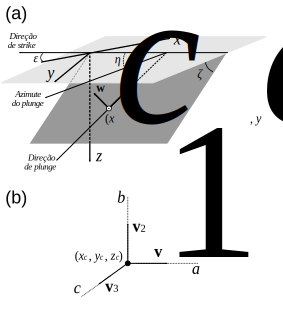
\includegraphics[width=12 cm,height=14.5 cm]{figures/structural_orientation_angles_port}
	\caption[Esquema representativo do sistema de coordenadas usado para representar um corpo elipsoidal.]{Esquema representativo do sistema de coordenadas usado para representar um corpo elipsoidal. a) Sistema de coordenadas principal com eixo $x$ apontado para norte, $y$ apontado para leste e $z$ para baixo. O plano cinza escuro contém o centro ($x_c$, $y_c$, $z_c$) (círculo branco) e dois vetores unitários, $u$ e $w$, que definem dois semi-eixos do corpo elipsoidal. Para elipsoides triaxiais e prolatos, $u$ e $w$ definem, respectivamente, os semi-eixos $a$ e $b$. Para elipsoides oblatos, $u$ e $w$ definem os semi-eixos $b$ e $a$, respectivamente. A \textit{direção de strike} é definida pela intersecção do plano cinza escuro e o plano horizontal (representado em cinza claro), que contém os eixos $x$ e $y$. O ângulo $\varepsilon$ entre "menos $x$" e a \textit{direção de strike} é chamado de \textit{strike}. O ângulo $\zeta$ entre o plano horizontal e o plano cinza escuro é chamado de \textit{dip}. A linha que contém o vetor unitário $u$ define a \textit{direção de plunge}. O ângulo $\eta$ entre a \textit{direção de strike} e a \textit{direção de plunge} é chamada de \textit{rake}. A projeção da \textit{direção de plunge} no plano horizontal é chamado de \textit{direção azimutal de plunge}. b) Sistema de coordenadas local com origem no centro do elipsoide ($x_c$, $y_c$, $z_c$) (ponto preto) e eixos definidos pelos vetores unitários $v_1$, $v_2$ e $v_3$. Estes vetores unitários definem os semi-eixos $a$, $b$ e $c$ dos elipsoides triaxiais, prolatos e oblatos da mesma forma. Para os  elipsoides triaxiais e prolatos, os vetores unitários $u$ e $w$, mostrados em  (a), coincidem com $v_1$ e $v_2$, respectivamente. Para elipsoides oblatos, os vetores unitários $u$ e $w$, mostrados em (a), coincidem com $v_2$ e $v_3$, respectivamente.}
	\label{fig:structural_orientation_angles}
\end{figure}

\section{Background Teórico}

Considere um corpo geológico localizado na crosta, que possua volume $\vartheta$, formato aproximadamente elipsoidal e que esteja imerso em um campo magnético uniforme $\mathbf{{H}_{0}}$ ($\unit{Am^{-1}}$) dado por:
\begin{equation}
\mathbf{H}_{0} = \| \mathbf{H}_{0} \| \left[
\begin{array}{c}
\cos I \: \cos D \\
\cos I \: \sin D \\
\sin I
\end{array}
\right] \: ,
\label{eq:H0}
\end{equation}
em que $\| \cdot \|$ é a norma Euclidiana e $D$ e $I$ são respectivamente, a declinação e inclinação do campo no sistema de coordenas principal (Fig. \ref{fig:structural_orientation_angles}a). Este campo uniforme representa a componente principal do campo magnético da Terra, que presume ser gerado na núcleo externo líquido da Terra. Ao longo deste trabalho, este campo uniforme é denominado \textit{campo geomagnético local}. Na ausência de correntes de condução, o campo magnético total $\mathbf{H}(\mathbf{r})$ (Eq. \ref{eq:A}) na posição $\mathbf{r}$ (Eq. \ref{eq:coord_transformation}) de um ponto no sistema de coordenadas principal é definido como \citep{sharma1966, eskola1980, reitz1992, sttraton2007}:
\begin{equation}
\mathbf{H}(\mathbf{r}) = \mathbf{H}_{0} - \nabla V(\mathbf{r}) \: ,
\label{eq:H}
\end{equation}
em que o segundo termo é o gradiente negativo do potencial magnético escalar $V(\mathbf{r})$ dado por:
\begin{equation}
V(\mathbf{r}) = -\frac{1}{4\pi} \iiint_{\vartheta} 
\mathbf{M}(\mathbf{r}^{\prime})^{\top} 
\nabla \left(
\frac{1}{\| \mathbf{r} - \mathbf{r}^{\prime} \|}
\right) \, dx^{\prime}dy^{\prime}dz^{\prime} \: .
\label{eq:phi-potential}
\end{equation}
Nesta equação, $\mathbf{r}^{\prime} = [\begin{array}{ccc} 
x^{\prime} & y^{\prime} & z^{\prime} \end{array} ]^{\top}$
é o vetor posição de um ponto localizado dentro do volume $\vartheta$, 
a integral é feita sobre as variáveis $x^{\prime}$, $y^{\prime}$ e 
$z^{\prime}$ e 
$\mathbf{M}(\mathbf{r}^{\prime})$ é o vetor de magnetização
(em $\unit{Am^{-1}}$).
A Eq. \ref{eq:phi-potential} é válida para pontos localizados dentro ou fora do corpo magnetizado \citep{dubois1896,sttraton2007, reitz1992}.

Considere que o corpo tem uma magnetização uniforme dada por:
\begin{equation}
\mathbf{M} = \mathbf{K} \, \mathbf{H}^{\dagger} \: ,
\label{eq:M-KH}
\end{equation}
em que $\mathbf{H}^{\dagger}$ é o campo magnético uniforme resultante em qualquer ponto dentro do corpo e $\mathbf{K}$ é um tensor de segunda ordem constante, que representa a susceptibilidade magnética do corpo. Esta é uma boa aproximação para corpos em temperatura ambiente, sujeitos a um campo indutor com intensidade $\leq 1$ \unit{mT} \citep{rochette1992}. Neste caso, o tensor de susceptibilidade $\mathbf{K}$ é representado, no sistema de coordenadas principal (Fig. \ref{fig:structural_orientation_angles}a), como:
\begin{equation}
\mathbf{K} = \mathbf{U}
\left[ \begin{array}{ccc}
k_{1} & 0 & 0 \\
0 & k_{2} & 0 \\
0 & 0 & k_{3} 
\end{array} \right] \mathbf{U}^{\top} \: ,
\label{eq:K}
\end{equation}
em que $k_{1} > k_{2} > k_{3}$ são as 
\textit{susceptibilidades principais} e $\mathbf{U}$ é
uma matriz ortogonal cujas colunas $\mathbf{u}_{i}$,
$i = 1, 2, 3$, são vetores unitários chamados de 
\textit{direções principais}.
Os vetores unitários $\mathbf{u}_{i}$ podem ser definidos de modo similar a que foi utilizada para definir os vetores
$\mathbf{v}_{1}$, $\mathbf{v}_{2}$,
e $\mathbf{v}_{3}$ (Eqs. \ref{eq:v1_triaxial_prolate},
\ref{eq:v2_triaxial_prolate}, \ref{eq:v3_triaxial_prolate},
\ref{eq:v1_oblate}, \ref{eq:v2_oblate}, e \ref{eq:v3_oblate}),
por um conjunto de ângulos $\varepsilon$, $\zeta$,
e $\eta$ e por conseguinte os ângulos auxiliares $\alpha$, $\gamma$ e $\delta$ (Eqs. \ref{eq:alpha}, \ref{eq:gamma}, e
\ref{eq:delta}).

Se as susceptibilidades principais são diferentes umas das outras, dizemos que o corpo possui uma anisotropia de susceptibilidade magnética (AMS). A AMS é geralmente associada à anisotropia magnetocristalina, que é causada por uma orientação preferencial dos grãos magnéticos dos minerais que formam a rocha \citep{fuller1963, uyeda1963, janak1972, hrouda1982, thompson1986, macdonald1987, rochette1992, dunlop1997, tauxe2003rudiments}. Para o caso particular em que as direções principais coincidem com os eixos do elipsoide, a matriz $\mathbf{U}$ é igual a matriz $\mathbf{V}$ (Eq. \ref{eq:A}). Outro caso particular importante, é quando a susceptibilidade é isotrópica e, consequentemente, as susceptibilidades principais $k_{1}$, $k_{2}$, e $k_{3}$ (Eq. \ref{eq:K}) são iguais a constante $\chi$. Neste caso, o tensor de susceptibilidades $\mathbf{K}$ (Eq. \ref{eq:K}) assume a forma particular:
\begin{equation}
\mathbf{K} = \chi \, \mathbf{I} \: ,
\label{eq:K-isotropic}
\end{equation}
em que $\mathbf{I}$ representa a matriz identidade.

Usando a magnetização $\mathbf{M}$ definida pela Eq. \ref{eq:M-KH}, o campo magnético total $\mathbf{H}(\mathbf{r})$ (Eq. \ref{eq:H}) pode ser reescrito como:
\begin{equation}
\mathbf{H}(\mathbf{r}) = \mathbf{H}_{0} 
- \mathbf{N}(\mathbf{r}) \, \mathbf{K} \, \mathbf{H}^{\dagger} \: ,
\label{eq:H-M-uniform}
\end{equation}
em que $\mathbf{N}(\mathbf{r})$ é uma matriz simétrica. O elemento ij de $\mathbf{N}(\mathbf{r})$ é dado por:
\begin{equation}
n_{ij}(\mathbf{r}) = 
\frac{1}{4\pi} \frac{\partial^{2} \, f(\mathbf{r})}
{\partial r_{i} \, \partial r_{j}} 
\: , \quad i = 1, 2, 3 \: , 
\quad j = 1, 2, 3 \: ,
\label{eq:nij}
\end{equation}
$r_{1} = x$, $r_{2} = y$, $r_{3} = z$ são os elementos do vetor posição $\mathbf{r}$ (Eq. \ref{eq:ellipsoid_surface}), 
e
\begin{equation}
f(\mathbf{r}) = \iiint_{\vartheta} 
\frac{1}{\| \mathbf{r} - \mathbf{r}^{\prime} \|}
\, dx^{\prime}dy^{\prime}dz^{\prime} \: .
\label{eq:f}
\end{equation}
Note que a função escalar $f(\mathbf{r})$ (Eq. \ref{eq:f}) é proporcional ao potencial gravitacional que seria produzido pelo corpo elipsoidal de volume $\vartheta$ se este tivesse uma densidade uniforme igual $1/G$, sendo $G$ a da constante gravitacional. Pode ser mostrado que os elementos $n_{ij}(\mathbf{r})$ são finitos tanto se $\mathbf{r}$ é um ponto dentro ou fora do volume $\vartheta$ \citep{peirce1902, webster1904}. A matriz $\mathbf{N}(\mathbf{r})$ (Eq. \ref{eq:H-M-uniform}) é chamada de \textit{tensor de depolarização} \citep{soliverez1981, soliverez2008}.

A parte seguinte desta dissertação é dedicada a descrever o campo magnético $\mathbf{H}(\mathbf{r})$ (Eq. \ref{eq:H-M-uniform}) nos pontos localizados tanto dentro como fora do volume $\vartheta$ do corpo elipsoidal. Entretanto, o desenvolvimento matemático é convenientemente feito no sistema de coordenadas local (Fig. \ref{fig:structural_orientation_angles}b).

\section{Transformação de coordenadas}

Para continuar a descrição da modelagem magnética de corpos elipsoidais, é conveniente definir duas importantes transformações de coordenadas. A primeira  transforma a função escalar $f(\mathbf{r})$ (Eq. \ref{eq:f}) do sistema de coordenadas principal para uma nova função escalar $\tilde{f}(\tilde{\mathbf{r}})$ no sistema de coordenada local.
A função $\tilde{f}(\tilde{\mathbf{r}})$ foi apresentada pela primeira vez por \citet{dirichlet1839} para descrever o potencial gravitacional produzido por elipsoides homogêneos. Posteriormente, diversos autores deduziram e usaram esta função para descrever os campos magnéticos e gravitacionais produzidos por elipsoides triaxiais, prolatos e oblatos \citep{maxwell1873, thomson1879, dubois1896, peirce1902, webster1904, kellogg1929, stoner1945, osborn1945, lowes1974,  peake1953, chang1961, clark1986, tejedor1995, sttraton2007}.
É conveniente usar $\tilde{f}^{\dagger}(\tilde{\mathbf{r}})$
e $\tilde{f}^{\ddagger}(\tilde{\mathbf{r}})$ para definir a função $\tilde{f}(\tilde{\mathbf{r}})$, calculada nos pontos $\tilde{\mathbf{r}}$ dentro e fora do volume $\vartheta$ do corpo elipsoidal, respectivamente.

A função escalar $\tilde{f}^{\dagger}(\tilde{\mathbf{r}})$
é dada por:
\begin{equation}
\tilde{f}^{\dagger}(\tilde{\mathbf{r}}) = \pi \, abc \, 
\int_{0}^{\infty} \left( 1 
- \frac{\tilde{x}^{2}}{a^{2} + u} 
- \frac{\tilde{y}^{2}}{b^{2} + u}
- \frac{\tilde{z}^{2}}{c^{2} + u} \right)
\frac{1}{R(u)} \, du \: , \quad \tilde{\mathbf{r}} \in V \: ,
\label{eq:fi-tilde}
\end{equation}
em 	que
\begin{equation}
R(u) = \sqrt{\left( a^{2} + u \right)\left( b^{2} + u \right)\left( c^{2} + u \right)} \: .
\label{eq:R}
\end{equation}
Esta função representa o potencial gravitacional que seria produzido pelo corpo elipsoidal nos pontos localizados dentro do volume $\vartheta$ se possuísse uma densidade uniforme igual ao inverso da constante gravitacional. Note que, para este caso, o potencial gravitacional é uma função quadrática das coordenadas espaciais $\tilde{x}$, $\tilde{y}$, e $\tilde{z}$. De forma similar, a função $\tilde{f}^{\ddagger}(\tilde{\mathbf{r}})$ é dada por:
\begin{equation}
\tilde{f}^{\ddagger}(\tilde{\mathbf{r}}) = \pi \, abc \, 
\int_{\lambda}^{\infty} \left( 1 
- \frac{\tilde{x}^{2}}{a^{2} + u} 
- \frac{\tilde{y}^{2}}{b^{2} + u}
- \frac{\tilde{z}^{2}}{c^{2} + u} \right)
\frac{1}{R(u)} \, du \: , \quad \tilde{\mathbf{r}} \not\in V \: ,
\label{eq:fe-tilde}
\end{equation}
em que $R(u)$ é definido pela Eq. \ref{eq:R} e o parâmetro $\lambda$ é definido de acordo com o tipo de elipsoide como uma função das coordenadas espaciais $\tilde{x}$, $\tilde{y}$, e $\tilde{z}$ (ver Apêndice B). Uma discussão detalhada sobre o parâmetro $\lambda$ pode ser encontrada em \citet[p.~234]{webster1904}, \citet[p.~184]{kellogg1929} e \citet{clark1986}.

A segunda importante transformação de coordenadas é definida com respeito a Eq. \ref{eq:H-M-uniform}. Usando a ortogonalidade de matriz $\mathbf{V}$ (Eqs. \ref{eq:V_triaxial_prolate}),
o campo magnético $\mathbf{H}(\mathbf{r})$ (Eq. \ref{eq:H-M-uniform}) pode ser transformado do sistema de coordenadas principal para o sistema de coordenadas local usando:
\begin{equation}
\underbrace{\mathbf{V}^{\top} \mathbf{H}(\mathbf{r})}_{\tilde{\mathbf{H}}(\tilde{\mathbf{r}})} = 
\underbrace{\mathbf{V}^{\top} \mathbf{H}_{0}}_{\tilde{\mathbf{H}}_{0}}
- \underbrace{\mathbf{V}^{\top} \mathbf{N}(\mathbf{r}) \mathbf{V}}
_{\tilde{\mathbf{N}}(\tilde{\mathbf{r}})} \;
\underbrace{\mathbf{V}^{\top} \mathbf{K} \mathbf{V}}
_{\tilde{\mathbf{K}}} \; 
\underbrace{\mathbf{V}^{\top} \mathbf{H}^{\dagger}}
_{\tilde{\mathbf{H}}^{\dagger}} \: ,
\label{eq:H-tilde}
\end{equation}
Nesta equação, o tensor de depolarização transformado $\tilde{\mathbf{N}}(\tilde{\mathbf{r}})$ é calculado como uma função do tensor de depolarização original $\mathbf{N}(\mathbf{r})$ (Eq. \ref{eq:H-M-uniform}). Neste caso, os elementos de $\tilde{\mathbf{N}}(\tilde{\mathbf{r}})$ são calculados como função das derivadas segundas da função $f(\mathbf{r})$ (Eq. \ref{eq:f}), que é definida no  sistema de coordenadas principal. Pode ser mostrado (Apêndice A), entretanto, que os elementos $\tilde{n}_{ij}(\tilde{\mathbf{r}})$ de
$\tilde{\mathbf{N}}(\tilde{\mathbf{r}})$ também podem ser calculados como:
\begin{equation}
\tilde{n}_{ij}(\tilde{\mathbf{r}}) = 
\frac{1}{4\pi} \frac{\partial^{2} \, \tilde{f}(\tilde{\mathbf{r}})}
{\partial \tilde{r}_{i} \, \partial \tilde{r}_{j}} 
\: , \quad i = 1, 2, 3 \: , \quad j = 1, 2, 3 \: ,
\label{eq:nij-tilde}
\end{equation}
em que $\tilde{r}_{1} = \tilde{x}$, $\tilde{r}_{2} = \tilde{y}$, 
e $\tilde{r}_{3} = \tilde{z}$ são os elementos do vetor transformado $\tilde{\mathbf{r}}$ (Eq. \ref{eq:coord_transformation})
e $\tilde{f}(\tilde{\mathbf{r}})$ é dada pela Eq. \ref{eq:fi-tilde}
ou \ref{eq:fe-tilde}, dependendo se $\tilde{\mathbf{r}}$ representa um ponto localizado dentro ou fora do volume $\vartheta$ do corpo elipsoidal.

\section{Tensores de depolarização transformados $\tilde{\mathbf{N}}(\tilde{\mathbf{r}})$}

\subsection{Tensor de depolarização $\tilde{\mathbf{N}}^{\dagger}$}

Sendo $\tilde{\mathbf{N}}^{\dagger}$ o tensor de depolarização transformado para o caso em que $\tilde{\mathbf{r}}$ (Eq. \ref{eq:coord_transformation}) representa um ponto dentro do corpo elipsoidal. Neste caso, os elementos de $\tilde{\mathbf{N}}^{\dagger}$ são calculados de acordo com a Eq. \ref{eq:nij-tilde}, com $\tilde{f}^(\tilde{\mathbf{r}})$ dada por $\tilde{f}^{\dagger}(\tilde{\mathbf{r}})$ (Eq. \ref{eq:fi-tilde}). 
Como mencionado anteriormente, $\tilde{f}^{\dagger}(\tilde{\mathbf{r}})$ (Eq. \ref{eq:fi-tilde}) é uma função quadrática das coordenadas espaciais $\tilde{x}$, $\tilde{y}$ and $\tilde{z}$. Consequentemente, os elementos $\tilde{n}^{\dagger}_{ij}$, $i = 1, 2, 3$, $j = 1, 2, 3$, de $\tilde{\mathbf{N}}^{\dagger}$ não dependem do vetor de posição transformado $\tilde{\mathbf{r}}$ (equação \ref{eq:coord_transformation}). Além disso, os elementos fora da diagonal são nulos e os elementos da diagonal são dados por \citep{stoner1945}: 
\begin{equation}
\tilde{n}^{\dagger}_{ii} = \frac{abc}{2}
\int_{0}^{\infty} \frac{1}{\left( e_{i}^{2} 
	+ u \right) R(u)} \, du \: , \quad i = 1, 2, 3 \: ,
\label{eq:n-tilde-dagger-ii}
\end{equation}
em que $R(u)$ é definido pela Eq. \ref{eq:R} e
$e_{1} = a$, $e_{2} = b$, e $e_{3} = c$. Estes elementos são comumente conhecidos como \textit{fatores de desmagnetização} e são definidos de acordo com o tipo de elipsoide. Observe que, de acordo com as Eqs. \ref{eq:H-tilde} e \ref{eq:N-tilde-VT-N-V},
\begin{equation}
\mathbf{N}(\mathbf{r}) = 
\mathbf{V} \, \tilde{\mathbf{N}}^{\dagger} \, 
\mathbf{V}^{\top} \: ,
\label{eq:N-V-N-dagger-VT}
\end{equation}
em que $\tilde{\mathbf{N}}^{\dagger}$ é uma matriz diagonal e $\mathbf{V}$ (Eqs. \ref{eq:V_triaxial_prolate}) é uma matriz ortogonal. Esta equação mostra que, para o caso particular em que $\mathbf{r}$ e consequentemente $\tilde{\mathbf{r}}$ representam um ponto dentro do volume $\vartheta$ do elipsoide, os elementos $\tilde{n}^{\dagger}_{ii}$ (Eq. \ref{eq:n-tilde-dagger-ii})
de $\tilde{\mathbf{N}}^{\dagger}$ representam os autovalores, enquanto as colunas de $\mathbf{V}$ representam os autovetores do tensor de depolarização $\mathbf{N}(\mathbf{r})$ definido no sistema de coordenadas principal.

\paragraph*{Elipsoides triaxiais}

Para elipsoides triaxiais (e.g., $a > b > c$), os fatores de desmagnetização obtidos a partir da Eq. \ref{eq:n-tilde-dagger-ii} são dados por:
\begin{equation}
\tilde{n}^{\dagger}_{11} = \frac{abc}
{\left( a^{2} - c^{2} \right)^{\frac{1}{2}} 
	\left( a^{2} - b^{2} \right)} 
\left[ F(\kappa, \phi) - E(\kappa, \phi) \right] \: ,
\label{eq:n-tilde-dagger-11-triaxial}
\end{equation}
\begin{equation}
\tilde{n}^{\dagger}_{22} = 
-\frac{abc}
{\left( a^{2} - c^{2} \right)^{\frac{1}{2}} 
	\left( a^{2} - b^{2} \right)} 
\left[ F(\kappa, \phi) - E(\kappa, \phi) \right] + 
\frac{abc}
{\left( a^{2} - c^{2} \right)^{\frac{1}{2}} 
	\left( b^{2} - c^{2} \right)} E(\kappa, \phi)
- \frac{c^{2}}{b^{2} - c^{2}}
\label{eq:n-tilde-dagger-22-triaxial}
\end{equation}
e
\begin{equation}
\tilde{n}^{\dagger}_{33} = 
-\frac{abc}
{\left( a^{2} - c^{2} \right)^{\frac{1}{2}} 
	\left( b^{2} - c^{2} \right)} E(\kappa, \phi) +
\frac{b^{2}}{b^{2} - c^{2}} \: ,
\label{eq:n-tilde-dagger-33-triaxial}
\end{equation}
em que
\begin{equation}
F(\kappa, \phi) = 
\int^{\phi}_{0} 
\frac{1}{\left( 1 - \kappa^{2} \sin^{2} \psi \right)^{\frac{1}{2}}}
d\psi \: ,
\label{eq:F-kappa-phi}
\end{equation}
e
\begin{equation}
E(\kappa, \phi) = 
\int^{\phi}_{0} 
\left( 1 - \kappa^{2} \sin^{2} \psi \right)^{\frac{1}{2}}
d\psi \: ,
\label{eq:E-kappa-phi}
\end{equation}
com $\kappa = \left[ \left( a^{2} - b^{2} \right) / 
\left( a^{2} - c^{2} \right) \right]^{\frac{1}{2}}$ e
$\cos \phi = c/a$.
As funções $F(\kappa, \phi)$ (Eq. \ref{eq:F-kappa-phi}) e 
$E(\kappa, \phi)$ (Eq. \ref{eq:E-kappa-phi}) são chamadas de integrais elípticas normais de Legendre de primeiro e segundo tipo, respectivamente. \citet{stoner1945} apresentou uma dedução detalhada dos fatores de desmagnetização $\tilde{n}^{\dagger}_{11}$ (Eq. \ref{eq:n-tilde-dagger-11-triaxial}), $\tilde{n}^{\dagger}_{22}$ (Eq. \ref{eq:n-tilde-dagger-22-triaxial}) e $\tilde{n}^{\dagger}_{33}$ (Eq. \ref{eq:n-tilde-dagger-33-triaxial}). \citet{clark1986} apresentou fórmulas similares.
Pode ser mostrado que estes fatores de desmagnetização satisfazem as condições $\tilde{n}^{\dagger}_{11} + \tilde{n}^{\dagger}_{22} + \tilde{n}^{\dagger}_{33} = 1$ e $\tilde{n}^{\dagger}_{33} > \tilde{n}^{\dagger}_{22} > \tilde{n}^{\dagger}_{11}$

\subparagraph*{Elipsoides prolatos}

Para elipsoides prolatos (e.g., $a > b = c$), os fatores de desmagnetização
obtidos a partir da Eq. \ref{eq:n-tilde-dagger-ii}, sendo dados por:
\begin{equation}
\tilde{n}^{\dagger}_{11} = \frac{1}{m^{2} - 1}
\left\lbrace \frac{m}{\left( m^{2} - 1 \right)^{\frac{1}{2}}}
\ln \left[ m + \left( m^{2} - 1 \right)^{\frac{1}{2}} \right]
- 1 \right\rbrace
\label{eq:n-tilde-dagger-11-prolate}
\end{equation}
e
\begin{equation}
\tilde{n}^{\dagger}_{22} = \frac{1}{2} \left(1 - \tilde{n}^{\dagger}_{11} \right) \: ,
\label{eq:n-tilde-dagger-22-prolate}
\end{equation}
em que $\tilde{n}^{\dagger}_{33} = \tilde{n}^{\dagger}_{22}$, 
e $m = a/b$.
As deduções detalhadas dos fatores de desmagnetização 
$\tilde{n}^{\dagger}_{11}$ (Eq. \ref{eq:n-tilde-dagger-11-prolate}) 
e $\tilde{n}^{\dagger}_{22}$ (Eq. \ref{eq:n-tilde-dagger-22-prolate})
podem ser encontradas, por exemplo, em \citet{stoner1945}. 
Essas fórmulas foram posteriormente apresentas por
\citet{emerson1985}, mas sem nenhuma prova matemática.
Pode ser mostrado que estes fatores de desmagnetização satisfazem as condições $\tilde{n}^{\dagger}_{11} + 2 \tilde{n}^{\dagger}_{22} = 1$ e $\tilde{n}^{\dagger}_{22} > \tilde{n}^{\dagger}_{11}$.

\subparagraph*{Elipsoides oblatos}

Para elipsoides oblatos (e.g., $a < b = c$), os fatores de desmagnetização obtidos 
a partir da Eq. \ref{eq:n-tilde-dagger-ii} são dados por:
\begin{equation}
\tilde{n}^{\dagger}_{11} = 
\frac{1}{1 - m^{2}} \left[
1 - \frac{m}{\left( 1 - m^{2} \right)^{\frac{1}{2}}} \cos^{-1}m
\right] \: ,
\label{eq:n-tilde-dagger-11-oblate}
\end{equation}
e
\begin{equation}
\tilde{n}^{\dagger}_{22} = 
\frac{1}{2} \left(1 - \tilde{n}^{\dagger}_{11}\right) ,
\label{eq:n-tilde-dagger-22-oblate}
\end{equation}
em que $\tilde{n}^{\dagger}_{33}=\tilde{n}^{\dagger}_{22}$ e $m = a/b$.
As deduções detalhadas dos fatores de desmagnetização 
podem ser encontradas em \citet{stoner1945}. Essas fórmulas
também podem ser encontradas em \citet{emerson1985}, mas sem nenhuma prova matemática.
A única diferença, entretanto, é que \citet{emerson1985} trocou o termo $\cos^{-1}$
por um termo $\tan^{-1}$, de acordo com a identidade trigonométrica
$\tan^{-1}x = \cos^{-1}(1/\sqrt{x^{2} + 1})$, $x > 0$. Pode ser mostrado que estes fatores de desmagnetização satisfazem as condições $\tilde{n}^{\dagger}_{11} + 2 \tilde{n}^{\dagger}_{22} = 1$ e $\tilde{n}^{\dagger}_{11} > \tilde{n}^{\dagger}_{22}$.

\subsection{Tensor de depolarização $\tilde{\mathbf{N}}^{\ddagger}(\tilde{\mathbf{r}})$}

Seja $\tilde{\mathbf{N}}^{\ddagger}(\mathbf{r})$ o tensor de depolarização definido para o caso em que $\tilde{\mathbf{r}}$ representa um ponto localizado fora do volume $\vartheta$ do corpo. Os elementos $\tilde{n}^{\ddagger}_{ij}(\tilde{\mathbf{r}})$,
$i = 1, 2, 3$, $j = 1, 2, 3$, de $\tilde{\mathbf{N}}^{\ddagger}(\tilde{\mathbf{r}})$ são calculadas de acordo com a Eq. \ref{eq:nij-tilde}, com 
$\tilde{f}(\tilde{\mathbf{r}})$ dado por $\tilde{f}^{\ddagger}(\tilde{\mathbf{r}})$
(Eq. \ref{eq:fe-tilde}).
Rearranjando as equações apresentadas por \citet{clark1986}, os elementos da diagonal $\tilde{n}^{\ddagger}_{ii}$
e os elementos fora da diagonal $\tilde{n}^{\ddagger}_{ij}$, $i = 1, 2, 3$,
$j = 1, 2, 3$, são dados por:
\begin{equation}
\tilde{n}^{\ddagger}_{ii}(\tilde{\mathbf{r}}) =
\frac{abc}{2}
\left( \frac{\partial \lambda}{\partial \tilde{r}_{i}} \, h_{i} \, \tilde{r}_{i}
- g_{i} \right)
\label{eq:n-tilde-ddagger-ii}
\end{equation}
e
\begin{equation}
\tilde{n}^{\ddagger}_{ij}(\tilde{\mathbf{r}}) =
\frac{abc}{2} \left(
\frac{\partial \lambda}{\partial \tilde{r}_{i}} \, h_{j} \, \tilde{r}_{j} 
\right) \: ,
\label{eq:n-tilde-dagger-ij}
\end{equation}
Em que
\begin{equation}
h_{i} = \frac{1}{\left( e_{i}^{2} + \lambda \right) R(\lambda)} \: ,
\label{eq:hi}
\end{equation}
\begin{equation}
g_{i} = \int_{\lambda}^{\infty} \frac{1}{\left( e_{i}^{2} + u \right) R(u)} du \: ,
\label{eq:gi}
\end{equation}
$e_{1} = a$, $e_{2} = b$, $e_{3} = c$, e 
$\frac{\partial \lambda}{\partial \tilde{r}_{i}}$
é definido no Apêndice B (Eq. \ref{eq:dlambda}).
As funções $g_{i}$ (Eq. \ref{eq:gi}) são definidas de acordo com
o tipo de elipsoide.

\subparagraph*{Elipsoides Triaxiais}

Para elipsoides triaxiais  (e.g., $a > b > c$), as funções
$g_{i}$ (Eq. \ref{eq:gi}) são dadas por
\citep{clark1986}:

\begin{equation}
g_{1} = \frac{2}{\left( a^{2} - b^{2} \right) \left( a^{2} - c^{2} \right)^{\frac{1}{2}}}
\left[ F(\kappa, \phi) - E(\kappa, \phi) \right] \: ,
\label{eq:g1-triaxial}
\end{equation}
\begin{equation}
g_{2} = \frac{2 \left( a^{2} - c^{2} \right)^{\frac{1}{2}}}
{\left( a^{2} - b^{2} \right)\left( b^{2} - c^{2} \right)}
\left[ E\left(\kappa, \phi \right) 
- \frac{\left( b^{2} - c^{2} \right)}{\left( a^{2} - c^{2} \right)}
F\left(\kappa, \phi \right) 
- \frac{\kappa^{2} \sin\phi \, \cos\phi}
{\left( 1 - \kappa^{2} \sin^{2}\phi \right)^{\frac{1}{2}}}
\right]
\label{eq:g2-triaxial}
\end{equation}
e
\begin{equation}
g_{3} = \frac{2}{\left( a^{2} - b^{2} \right) \left( a^{2} - c^{2} \right)^{\frac{1}{2}}}
\left[ \frac{\sin\phi \left( 1 - \kappa^{2} \sin^{2}\phi \right)^{\frac{1}{2}}}
{\cos\phi}  - E\left(\kappa, \phi \right) \right]
\: ,
\label{eq:g3-triaxial}
\end{equation}
em que $F(\kappa, \phi)$ e $E(\kappa, \phi)$ são, respectivamente, definidas pelas
Eqs. \ref{eq:F-kappa-phi} e \ref{eq:E-kappa-phi},
mas com
$\sin \phi = \sqrt{\left( a^{2} - c^{2} \right)/\left( a^{2} + \lambda \right)}$.

\subparagraph*{Elipsoides prolatos}


Para elipsoides prolatos (e.g., $a > b = c$), as funções
$g_{i}$ (Eq. \ref{eq:gi}) são dadas por:
\begin{equation}
g_{1} =  \frac{2}{\left( a^{2} - b^{2} \right)^{\frac{3}{2}}}
\left\lbrace
\ln \left[ \frac{\left( a^{2} - b^{2} \right)^{\frac{1}{2}} + 
	\left( a^{2} + \lambda \right)^{\frac{1}{2}}}{
	\left( b^{2} + \lambda \right)^{\frac{1}{2}}} \right] -
\left( \frac{a^{2} - b^{2}}{a^{2} + \lambda} \right)^{\frac{1}{2}}
\right\rbrace
\label{eq:g1-prolate}
\end{equation}
e
\begin{equation}
g_{2} =  \frac{1}{\left( a^{2} - b^{2} \right)^{\frac{3}{2}}}
\left\lbrace
\frac{\left[ \left( a^{2} - b^{2} \right)
	\left( a^{2} + \lambda \right) \right]^{\frac{1}{2}}}
{b^{2} + \lambda} -
\ln \left[ \frac{\left( a^{2} - b^{2} \right)^{\frac{1}{2}} + 
	\left( a^{2} + \lambda \right)^{\frac{1}{2}}}{
	\left( b^{2} + \lambda \right)^{\frac{1}{2}}} \right]
\right\rbrace \: ,
\label{eq:g2-prolate}
\end{equation}
em que $g_{3} = g_{2}$.
Estas fórmulas podem ser obtidas manipulando apropriadamente aquelas
apresentadas por \cite{emerson1985}.


\subparagraph*{Elipsoides oblatos}


Para elipsoides oblatos (i.e., $a < b = c$), as funções
$g_{i}$ (Eq. \ref{eq:gi}) são dadas por:
\begin{equation}
g_{1} =  \frac{2}{\left( b^{2} - a^{2} \right)^{\frac{3}{2}}}
\left\lbrace
\left( \frac{b^{2} - a^{2}}{a^{2} + \lambda}\right)^{\frac{1}{2}} -
\tan^{-1} \left[ \left( \frac{b^{2} - a^{2}}{a^{2} + \lambda}\right)^{\frac{1}{2}} \right]
\right\rbrace
\label{eq:g1-oblate}
\end{equation}
e
\begin{equation}
g_{2} =  \frac{1}{\left( b^{2} - a^{2} \right)^{\frac{3}{2}}}
\left\lbrace
\tan^{-1} \left[ \left( \frac{b^{2} - a^{2}}{a^{2} + \lambda}\right)^{\frac{1}{2}} \right] -
\frac{\left[ \left( b^{2} - a^{2} \right)
	\left( a^{2} + \lambda \right) \right]^{\frac{1}{2}}}
{b^{2} + \lambda}
\right\rbrace \: ,
\label{eq:g2-oblate}
\end{equation}
em que $g_{3} = g_{2}$.
De forma similar ao caso prolato mostrado anteriormente,
estas fórmulas podem ser obtidas manipulando apropriadamente aquelas
apresentadas por \citep{emerson1985}.

\section{Campo magnético interno e magnetização}

Utilizando a Eq. \ref{eq:H-tilde}, é possível definir o campo magnético uniforme resultante $\tilde{\mathbf{H}}^{\dagger}$ dentro do corpo como:
\begin{equation}
\begin{split}
\tilde{\mathbf{H}}^{\dagger}
&= \tilde{\mathbf{H}}_{0} - \tilde{\mathbf{N}}^{\dagger} \, \tilde{\mathbf{K}} \, \tilde{\mathbf{H}}^{\dagger} \\
&= 
\left( \mathbf{I} + \tilde{\mathbf{N}}^{\dagger} \, \tilde{\mathbf{K}} \right)^{-1}
\tilde{\mathbf{H}}_{0}
\end{split} \: ,
\label{eq:Hi-tilde}
\end{equation}
em que $\mathbf{I}$ é a matriz identidade e
$\tilde{\mathbf{N}}^{\dagger}$ está definido na subseção 2.4.1.

Transformando o campo magnético $\tilde{\mathbf{H}}^{\dagger}$ para o sistema de coordenadas principal, obtém-se:
\begin{equation}
\underbrace{\mathbf{V}^{\top} \tilde{\mathbf{H}^{\dagger}}}_{\mathbf{H}^{\dagger}} =  
\underbrace{\mathbf{V} \left ( \mathbf{I} + \tilde{\mathbf{N}}^{\dagger} \, \tilde{\mathbf{K}} \right)^{-1} \mathbf{V}^{\top}}_{\Upsilon}
\underbrace{\mathbf{V} \tilde{\mathbf{H}}_{0}}_{\mathbf{H}_{0}}
\label{eq:Hi}
\end{equation}

\begin{equation}
{\mathbf{H}^{\dagger}} =  
{\Upsilon} \, 
{\mathbf{H}_{0}} \: ,
\label{eq:Hi-p}
\end{equation}
em que
\begin{equation}
{\mathbf{H}^{\dagger}} =  \mathbf{V}^{\top} \tilde{\mathbf{H}^{\dagger}} \: ,
\label{eq:Hi-p-separado}
\end{equation}

\begin{equation}
{\Upsilon} =  {\mathbf{V} \left ( \mathbf{I} + \tilde{\mathbf{N}}^{\dagger} \, \tilde{\mathbf{K}} \right)^{-1} \mathbf{V}^{\top}} \:
\label{eq:upsilon-separado}
\end{equation}
e
\begin{equation}
{\mathbf{H}_{0}} =  {\mathbf{V} \tilde{\mathbf{H}}_{0}} \: .
\label{eq:h0-separado}
\end{equation}

Pré-multiplicando o campo interno uniforme $\tilde{\mathbf{H}}^{\dagger}$
(Eq. \ref{eq:Hi-p}) pelo tensor de susceptibilidade transformado ${\mathbf{K}}$ (Eq. \ref{eq:K}) obtemos:
\begin{equation}
\begin{split}
\tilde{\mathbf{M}} 
&= \tilde{\mathbf{K}} 
\left( \mathbf{I} + \tilde{\mathbf{N}}^{\dagger} \, \tilde{\mathbf{K}} \right)^{-1}
\tilde{\mathbf{H}}_{0} \\
&=  
\left( \mathbf{I} + \tilde{\mathbf{K}} \, \tilde{\mathbf{N}}^{\dagger} \right)^{-1}
\tilde{\mathbf{K}} \, \tilde{\mathbf{H}}_{0}
\end{split} \: ,
\label{eq:M-tilde}
\end{equation}
em que $\mathbf{M}$ representa a magnetização definida no sistema de coordenadas principal (Eqs. \ref{eq:M-KH}). A identidade matricial usada para obter a segunda linha da Eq. \ref{eq:M-tilde} é dada por \citet[p. ~151]{searle1982}.

De forma similar a transformação de coordenadas da Eq. \ref{eq:Hi-p}, podemos reescrever a equação \ref{eq:M-tilde} no sistema principal:
\begin{equation}
{\mathbf{M}} =
{\Lambda} \,
{\mathbf{K}} \,
{\mathbf{H}_{0}}
\label{eq:M-p}
\end{equation}
em que
\begin{equation}
\mathbf{\Lambda} = {\mathbf{V} \left (\mathbf{I} + \tilde{\mathbf{K}} \, \tilde{\mathbf{N}}^{\dagger} \right)^{-1} \mathbf{V}^{\top}} \, .
\label{eq:Lambda}
\end{equation}

A equação \ref{eq:M-p} pode ser facilmente generalizada para o caso em que o elipsoide também possui uma magnetização remanente uniforme ${\mathbf{M}}_{R}$. Primeiramente, consideremos que a magnetização remanente uniforme satisfaz a condição ${\mathbf{H}}_{A} = {\mathbf{K}}^{-1} {\mathbf{M}}_{R}$, em que ${\mathbf{H}}_{A}$ representa um campo uniforme hipotético. Assim, se assumirmos que ${\mathbf{H}}_{0}$,
nas Eqs. \ref{eq:Hi-p} e \ref{eq:M-p}, é de fato a soma do campo magnético uniforme ${\mathbf{H}}_{0}$ e o campo hipotético ${\mathbf{H}}_{A}$, obtemos a seguinte equação generalizada:
\begin{equation}
{\mathbf{M}} =  
\mathbf{\Lambda} \,
\left( {\mathbf{K}} \, {\mathbf{H}}_{0} + {\mathbf{M}}_{R} \right) \: ,
\label{eq:M-p-remanence}
\end{equation}
em que $\mathbf{{\Lambda}}$ é dado na equação \ref{eq:Lambda}.

A equação \ref{eq:M-p-remanence} é consistente com aquela apresentada por \citet[Eq. ~38]{clark1986} e mostra o efeito combinado da anisotropia de susceptibilidade magnética (AMS) e da anisotropia de forma. A AMS é representada pelo tensor de susceptibilidade $\mathbf{K}$ (Eq. \ref{eq:K}) e reflete a orientação preferencial dos minerais magnéticos que formam o corpo. O tensor de susceptibilidade aparece na Eq. \ref{eq:M-p-remanence}, definido no sistema de coordenadas principal (Fig. \ref{fig:structural_orientation_angles}a), e na Eq. \ref{eq:M-tilde}, definido no sistema de coordenada local
(Fig. \ref{fig:structural_orientation_angles}b). A anisotropia de forma, é representada pelo tensor de depolarização $\tilde{\mathbf{N}}^{\dagger}$ e reflete a desmagnetização associada à forma do corpo. Note que a magnetização resultante, $\mathbf{M}$ (Eq. \ref{eq:M-p-remanence}), não necessariamente possui a mesma direção do campo indutor $\mathbf{H}_{0}$
(Eq. \ref{eq:H0}). A diferença angular entre a magnetização resultante e o campo indutor depende do efeito combinado da anisotropia de susceptibilidade magnética e da anisotropia de forma.

Para o caso particular em que a susceptibilidade é isotrópica,
o tensor de susceptibilidade é definido de acordo com a Eq. \ref{eq:K-isotropic}.
Neste caso, a magnetização $\mathbf{M}$ (Eqs. \ref{eq:M-KH} e \ref{eq:M-p-remanence}),
referida no sistema de coordenada principal (Fig. \ref{fig:structural_orientation_angles}a),
e a matriz $\mathbf{\Lambda}$ (Eq. \ref{eq:Lambda})
podem ser reescritas como segue:
\begin{equation}
\mathbf{M} = \mathbf{\Lambda} \left( \chi \, \mathbf{H}_{0} +
\mathbf{M}_{R} \right) \: ,
\label{eq:M-K-isotropic}
\end{equation}
e
\begin{equation}
\mathbf{\Lambda} = \mathbf{V}
\left( \mathbf{I} + \chi \, \tilde{\mathbf{N}}^{\dagger} \right)^{-1}
\mathbf{V}^{\top} \: .
\label{eq:Lambda-K-isotropic}
\end{equation}

Desconsiderando a transformação de coordenadas representada pela matriz $\mathbf{V}$ (Eq. \ref{eq:A}),
esta equação está perfeitamente de acordo com as apresentadas por \citet[Eqs. ~13--15]{guo2001}.
O primeiro termo, dependente do campo indutor $\mathbf{H}_{0}$
(Eq. \ref{eq:H0}), 
representa a magnetização induzida, enquanto o termo dependente de
$\mathbf{M}_{R}$ é a magnetização remanente resultante.
A equação \ref{eq:M-K-isotropic} mostra que, como apontado por vários autores
\citep[e.g.,][]{maxwell1873, dubois1896, stoner1945, clark1986, sttraton2007},
a magnetização induzida se opõe ao campo indutor 
quando este é paralelo a um eixo do elipsoide, 
independente do tipo de elipsoide. Por outro lado, a
magnetização não é necessariamente paralela ao campo indutor quando este não está alinhado a um eixo do elipsoide.
Se adicionalmente considerarmos que $\chi << 1$, a matriz
$\mathbf{\Lambda}$ (Eq. \ref{eq:Lambda-K-isotropic})
se aproxima da matriz identidade e a magnetização
$\mathbf{M}$ (Eq. \ref{eq:M-K-isotropic})
pode ser aproximada por:
\begin{equation}
\breve{\mathbf{M}} = \chi \, \mathbf{H}_{0} +
\mathbf{M}_{R} \: ,
\label{eq:M-approx}
\end{equation}
que é a equação clássica que descreve a magnetização resultante em geofísica aplicada \citep[p. ~89]{blakely1996}.
Notemos que, neste caso particular, a magnetização induzida
é paralela ao campo indutor $\mathbf{H}_{0}$ (Eq. \ref{eq:H0}),
seja ele paralelo a algum eixo do elipsoide ou não.
Usualmente, Eq. \ref{eq:M-approx}
é considerada uma boa aproximação quando $\chi \leq 0.1$ SI.
Apesar de este valor ser amplamente utilizado na literatura,
houve poucas investigações empíricas e/ou teóricas sobre como este valor foi determinado.

\subsubsection{Relação entre $\chi$ e o erro da magnetização}

No caso da susceptibilidade isotrópica, a magnetização resultante
$\mathbf{M}$ (Eq. \ref{eq:M-K-isotropic}) pode ser determinada resolvendo o seguinte sistema linear:
\begin{equation}
\mathbf{\Lambda}^{-1} \, \mathbf{M} = \chi \, \mathbf{H}_{0} +
\mathbf{M}_{R} \: ,
\label{eq:M-K-isotropic-inverse-Lambda}
\end{equation}
em que, de acordo com a Eq. \ref{eq:Lambda-K-isotropic},
\begin{equation}
\mathbf{\Lambda}^{-1} = \mathbf{V}
\left( \mathbf{I} + \chi \, \tilde{\mathbf{N}}^{\dagger} \right)
\mathbf{V}^{\top} \: .
\label{eq:inverse-Lambda}
\end{equation}

Considere uma matriz $\delta \mathbf{\Lambda}^{-1}$ dada por:
\begin{equation}
\delta \mathbf{\Lambda}^{-1} = \mathbf{\Lambda}^{-1} - \mathbf{I}
\label{eq:perturbed-inverse-Lambda}
\end{equation}
e, similarmente, um vetor de magnetização perturbado $\delta \mathbf{M}$
dado por:
\begin{equation}
\delta \mathbf{M} = \mathbf{M} - \breve{\mathbf{M}} \: ,
\label{eq:perturbed-M}
\end{equation}
Usando estas duas equações, podemos reescrever a magnetização aproximada $\breve{\mathbf{M}}$ (Eq. \ref{eq:M-approx}) como:
\begin{equation}
\left( \mathbf{\Lambda}^{-1} - \delta \mathbf{\Lambda}^{-1} \right)
\left( \mathbf{M} - \delta \mathbf{M} \right) = 
\chi \, \mathbf{H}_{0} +
\mathbf{M}_{R} \: .
\label{eq:perturbed-system}
\end{equation}
Subtraindo a magnetização verdadeira 
$\mathbf{M}$ (Eq. \ref{eq:M-K-isotropic-inverse-Lambda})
deste sistema linear (Eq. \ref{eq:perturbed-system})
e rearranjando os termos, obtemos o seguinte sistema linear para a magnetização perturbada $\delta \mathbf{M}$
(Eq. \ref{eq:perturbed-M}):
\begin{equation}
\delta \mathbf{M} = - \delta \mathbf{\Lambda}^{-1} \mathbf{M} \: .
\label{eq:perturbed-M-system}
\end{equation}

Usando o conceito de norma de um vetor e seu correspondente operador de norma \citep{demmel1997, golub2013}, podemos usar a Eq.
\ref{eq:perturbed-M-system} para escrever a seguinte desigualdade:
\begin{equation}
\| \delta \mathbf{M} \| \leq
\| \delta \mathbf{\Lambda}^{-1} \| \, \| \mathbf{M} \| \: ,
\label{eq:perturbed-M-inequality1}
\end{equation}
e portanto:
\begin{equation}
\frac{\| \delta \mathbf{M} \|}{\| \mathbf{M} \|} \leq
\| \delta \mathbf{\Lambda}^{-1} \| \: .
\label{eq:perturbed-M-inequality}
\end{equation}
em que $\| \delta \mathbf{M} \|$ e $\| \mathbf{M} \|$
representam a norma Euclidiana (ou norma-2) e o termo 
$\| \delta \mathbf{\Lambda}^{-1} \|$ representa a norma-2 da matriz
de $\delta \mathbf{\Lambda}^{-1}$.
Usando as Eqs. \ref{eq:inverse-Lambda} e \ref{eq:perturbed-inverse-Lambda}
e a invariância da norma-2 de matrizes em relação a matrizes ortogonais
\citep{demmel1997, golub2013}, definimos
$\| \delta \mathbf{\Lambda}^{-1} \|$ como:
\begin{equation}
\| \delta \mathbf{\Lambda}^{-1} \| = \chi \,
\tilde{n}^{\dagger}_{max} \: ,
\label{eq:norm-perturbed-inverse-Lambda}
\end{equation}
em que $\tilde{n}^{\dagger}_{max}$ é o fator de desmagnetização
associado ao menor semi-eixo do elipsoide.
Para um elipsoide triaxial, 
$\tilde{n}^{\dagger}_{max} \equiv \tilde{n}^{\dagger}_{33}$
(Eq. \ref{eq:n-tilde-dagger-33-triaxial}). Para um elipsoide prolato,
$\tilde{n}^{\dagger}_{max} \equiv \tilde{n}^{\dagger}_{22}$
(Eq. \ref{eq:n-tilde-dagger-22-prolate}). 
Para um elipsoide oblato,
$\tilde{n}^{\dagger}_{max} \equiv \tilde{n}^{\dagger}_{11}$
(Eq. \ref{eq:n-tilde-dagger-11-oblate}).
É importante lembrar que, independentemente do tipo de elipsoide, $\tilde{n}^{\dagger}_{max}$ é
uma função escalar dos semi-eixos do elipsoide.
Na Eq. \ref{eq:perturbed-M-inequality}, a razão
$\| \delta \mathbf{M} \| \, \| \mathbf{M} \|^{-1}$ representa o
\textit{erro relativo} da magnetização aproximada
$\breve{\mathbf{M}}$ (Eq. \ref{eq:M-approx}) com relação a magnetização verdadeira
$\mathbf{M}$ (Eqs. \ref{eq:M-K-isotropic}
e \ref{eq:M-K-isotropic-inverse-Lambda}).

Dado um erro relativo fixo
e um elipsoide com determinados semi-eixos, podemos usar a desigualdade representada pela 
Eq. \ref{eq:norm-perturbed-inverse-Lambda}
para definir
\begin{equation}
\chi_{max} = \frac{\epsilon}{\tilde{n}^{\dagger}_{max}} \: ,
\label{eq:max-chi}
\end{equation}
que representa a máxima susceptibilidade isotrópica que o corpo elipsoidal
pode assumir para garantir um erro relativo menor que ou igual a $\epsilon$ na magnetização resultante calculada.
Para susceptibilidades isotrópicas maiores que $\chi_{max}$,
não é possível garantir que o erro relativo na magnetização aproximada
$\breve{\mathbf{M}}$ (Eq. \ref{eq:M-approx}) com relação a magnetização verdadeira
$\mathbf{M}$ (Eqs. \ref{eq:M-K-isotropic} e \ref{eq:M-K-isotropic-inverse-Lambda})
seja menor ou igual a $\epsilon$. A comunidade geocientífica tem usado $\chi_{max} = 0.1$ SI
como um valor limite para negligenciar a desmagnetização e, consequentemente, utilizar a magnetização
$\breve{\mathbf{M}}$ (Eq. \ref{eq:M-approx}) como uma boa aproximação para a magnetização
verdadeira $\mathbf{M}$ (Eqs. \ref{eq:M-K-isotropic} e \ref{eq:M-K-isotropic-inverse-Lambda}).
Por outro lado, a equação \ref{eq:max-chi}, define $\chi_{max}$ como uma função dos semi-eixos do elipsoide,
de acordo com um erro relativo $\epsilon$ especificado pelo intérprete.

\section{Campo magnético externo e anomalia de campo-total}

O campo magnético $\Delta {\mathbf{H}}({\mathbf{r}})$ produzido por um elipsoide nos pontos externos
como a diferença entre o campo resultante ${\mathbf{H}}({\mathbf{r}})$ 
e o campo uniforme ${\mathbf{H}}_{0}$ (Eq. \ref{eq:H0}). De acordo com a Eq. \ref{eq:H}:
\begin{equation}
\underbrace{\mathbf{H} - \mathbf{H}_0}_{\Delta {\mathbf{H}}({\mathbf{r}})} =  - {\mathbf{N}}({\mathbf{r}}) \, \underbrace{\mathbf{K} \, \mathbf{H}^{\dagger}}_{\mathbf{M}}
\label{eq:delta-H1}
\end{equation}
Como é fora do elipsoide:
\begin{equation}
{\mathbf{N}}({\mathbf{r}}) = {\mathbf{N}}^{\ddagger}({\mathbf{r}}) \: ,
\label{eq:N-out}
\end{equation}
Logo:
\begin{equation}
\Delta {\mathbf{H}}({\mathbf{r}}) = 
- {\mathbf{N}}^{\ddagger}({\mathbf{r}}) \, {\mathbf{M}} \: ,
\label{eq:delta-H}
\end{equation}
em que ${\mathbf{N}}^{\ddagger}({\mathbf{r}})$ é dado por:
\begin{equation}
{\mathbf{N}}^{\ddagger}({\mathbf{r}}) = 
\mathbf{V} \, \tilde{{\mathbf{N}}}^{\ddagger}({\mathbf{r}}) \, \mathbf{V}^{\top}
\label{eq:n-p} \: ,
\end{equation}
sendo $\mathbf{V}$ definida na Eq. \ref{eq:V_triaxial_prolate} e $\mathbf{N^{\ddagger}}$ definida a partir dos elementos dados nas Eqs. \ref{eq:n-tilde-ddagger-ii} e \ref{eq:n-tilde-dagger-ij}. A equação \ref{eq:delta-H} fornece o campo magnético (em \unit{A \, m^{-1}}). Entretanto, na geofísica, é mais usual utilizar a indução magnética, que é definida em \unit{nT}. Esta conversão pode ser facilmente feita multiplicando a Eq. \ref{eq:delta-H} por $k_{m}~=~10^{9}~\mu_{0}$, em que $\mu_{0}$ representa a constante magnética (em \unit{H \, m^{-1}}).

Para aplicações geofísicas, é preferível calcular a anomalia de campo total produzida por fontes magnéticas. Esta quantidade escalar é definida como \citep{blakely1996}:
\begin{equation}
\Delta {T}({\mathbf{r}}) = \| 
{\mathbf{B}}_{0} + \Delta {\mathbf{B}}({\mathbf{r}}) \|
- \| {\mathbf{B}}_{0} \| \: ,
\label{eq:delta-T-tilde}
\end{equation}
em que ${\mathbf{B}}_{0} = k_{m} \, {\mathbf{H}}_{0}$
e $\Delta {\mathbf{B}}({\mathbf{r}}) = 
k_{m} \, \Delta {\mathbf{H}}({\mathbf{r}})$, com ${\mathbf{H}}_{0}$ definido na eq \ref{eq:H0} e $\Delta {\mathbf{H}}({\mathbf{r}})$ definido na Eq. \ref{eq:delta-H}.
Em situações práticas, entretanto, 
$\| {\mathbf{B}}_{0} \| >> \| \Delta {\mathbf{B}}({\mathbf{r}}) \|$
e, consequentemente, a seguinte aproximação é válida \citep{blakely1996}:
\begin{equation}
\Delta {T}({\mathbf{r}}) \approx  
\frac{{\mathbf{B}}_{0}^{\top} \Delta {\mathbf{B}}({\mathbf{r}})}{\| {\mathbf{B}}_{0} \|} \: .
\label{eq:delta-T-tilde-approx}
\end{equation}
  \chapter{Implementação computacional}

A implementação computacional das rotinas desenvolvidas nesta dissertação foi feita em linguagem livre Python, que é gratuita, bem documentada, roda em praticamente todos os sistemas operacionais e vem sendo amplamente utilizada pela comunidade científica.  
As rotinas desenvolvidas ao longo deste trabalho foram baseadas no pacote \textit{Fatiando a Terra} \citet{uieda-proc-scipy-2013}, que é livre, de código aberto e desenvolvido para modelagem e inversão em geofísica. A documentação e as instruções para instalação da versão mais atual do \textit{Fatiando a Terra} podem ser encontrados em http://www.fatiando.org.
As rotinas desenvolvidas aqui estão livremente disponibilizadas no Github pelo link: https://github.com/DiegoTaka/ellipsoid-magnetic.

A Figura \ref{fig:Cookbook_Triaxial} exemplifica como calcular a anomalia de campo total $\Delta T (\mathbf{r})$ (Eq. \ref{eq:delta-T-tilde-approx}) gerada por um elipsoide triaxial.
Como mostrado neste exemplo, é necessário importar outros módulos do \textit{Fatiando a Terra} antes de criar o modelo elipsoidal desejado.
A parte \textit{``The local-geomagnetic field"} define a intensidade ($nT$), inclinação e declinação $(º)$ do campo geomagnético local.
A variável \textit{``model"} contém um objeto da classe \textit{``EllipsoidTriaxial"}, que foi desenvolvida neste trabalho como parte do subpacote \textit{``mesher"} do Fatiando a Terra. Esta variável contém os parâmetros que definem o modelo de elipsoide triaxial. Os parâmetros são, respectivamente: posição $x_c$, $y_c$ e $z_c$ ($m$) do centro do corpo, semi-eixos $a$, $b$ e $c$ ($m$), orientações de \textit{strike, dip e rake} $(º)$ e um dicionário que contém as propriedades físicas do modelo. O item \textit{``remanence"} contém a intensidade ($A/m$), inclinação e declinação $(º)$ do vetor de magnetização remanente $\mathbf{M}_{R}$ (Eq. \ref{eq:M-p-remanence}). O item \textit{`k'} contém as susceptibilidades principais $k1$, $k2$ e $k3$ (Eq. \ref{eq:K}) e as orientações \textit{strike}, \textit{dip} e \textit{rake} utilizadas para calcular os vetores unitários $\mathbf{u}_{1}$, $\mathbf{u}_{2}$ e $\mathbf{u}_{3}$ que formam as colunas da matriz ortogonal $\mathbf{U}$ (Eq. \ref{eq:K}). Os vetores foram calculados utilizando-se as Eqs. \ref{eq:v1_triaxial_prolate},
\ref{eq:v2_triaxial_prolate}, \ref{eq:v3_triaxial_prolate}.
As linhas seguintes definem as coordenadas dos pontos $(x, y, z)$ em que será calculada a anomalia de campo total produzida pelo modelo elipsoidal.
Para tanto, utilizou-se o subpacote \textit{``gridder"} do Fatiando a Terra. Neste exemplos, os pontos estão distribuídos em uma grade regular de 200 x 200 (definida pela variável \textit{``shape"}), sobre um plano horizontal em $z = 0$ m. Os pontos são calculados sobre uma área que varia de -5000 até 5000 metros ao longo das direções $x$ e $y$, tal como definido pela variável \textit{``area"}.
As coordenadas são armazenadas nos \textit{``numpy arrays"}: \textit{``xp", ``yp" e ``zp"}. Em seguida, a anomalia de campo total é calculada utilizando-se a rotina \textit{``tf\underline{ }c"}. Esta função está contida no módulo \textit{``ellipsoid\underline{ }triaxial"}, que foi desenvolvido neste trabalho como parte do subpacote \textit{``gravmag"} do Fatiando a Terra. As linhas finais do exemplo mostrado na Fig. \ref{fig:Cookbook_Triaxial} são para plotar a anomalia de campo total produzida pelo modelo elipsoidal utilizando-se o módulo \textit{``mpl"}, que está contido no subpacote \textit{``vis"} do Fatiando a Terra.

A Fig. \ref{fig:anomaly_exemplo} mostra o resultado produzido pelo código da Fig. \ref{fig:Cookbook_Triaxial}. A Fig. \ref{fig:func_triaxial} mostra o código fonte da rotina \textit{``tf\underline{ }c"} (Fig. \ref{fig:Cookbook_Triaxial}) utilizada para calcular a anomalia de campo total mostrada na Fig. \ref{fig:anomaly_exemplo}.
As rotinas também contam com classes que separam os três tipos de elipsoides tratados neste trabalho.

É importante ressaltar que diversos cálculos são feitos com auxílio de bibliotecas do \textit{Python} como o \textit{Scipy} \citet{scipy}, \textit{Matplotlib} \citet{matplotlib} e do pacote \textit{NumPy} \citet{numpy}.
Uma nota a respeito das funções \textit{scipy.special.ellipkinc} e \textit{scipy.special.ellipeinc} do pacote SciPy para o cálculo das integrais elípticas normais incompletas de Legendre de primeiro e segundo tipo (Eqs. \ref{eq:F-kappa-phi} e \ref{eq:E-kappa-phi}): a variável $\kappa$ das funções $F(\kappa, \phi)$ e $E(\kappa, \phi)$ já deve ser elevada ao quadrado.

Tal como definido anteriormente, a soma dos fatores de desmagnetização deve ser igual à 1 (um), independente do tamanho dos eixos e do tipo de elipsoide. Para verificar esta propriedade, foram gerados 200 elipsoides triaxiais com semi-eixos $a = a_0 +u, \, b = b_0+u$ e $c = c_0+u$, em que $a_0=500$ m, $b_0=100$ m, $c_0=50$ m e $500  \le u \le 30000$ m. A Fig. \ref{fig:teste_n_soma} mostra a soma dos fatores de desmagnetização $\tilde{n}^{\dagger}_{11}$, $\tilde{n}^{\dagger}_{22}$ e $\tilde{n}^{\dagger}_{33}$ calculados pelas Eqs. \ref{eq:n-tilde-dagger-11-triaxial}, \ref{eq:n-tilde-dagger-22-triaxial} e \ref{eq:n-tilde-dagger-33-triaxial} para este conjunto de elipsoides e serve como validação de parte das rotinas apresentadas neste trabalho.

\begin{figure}[hbt!]
	\centering 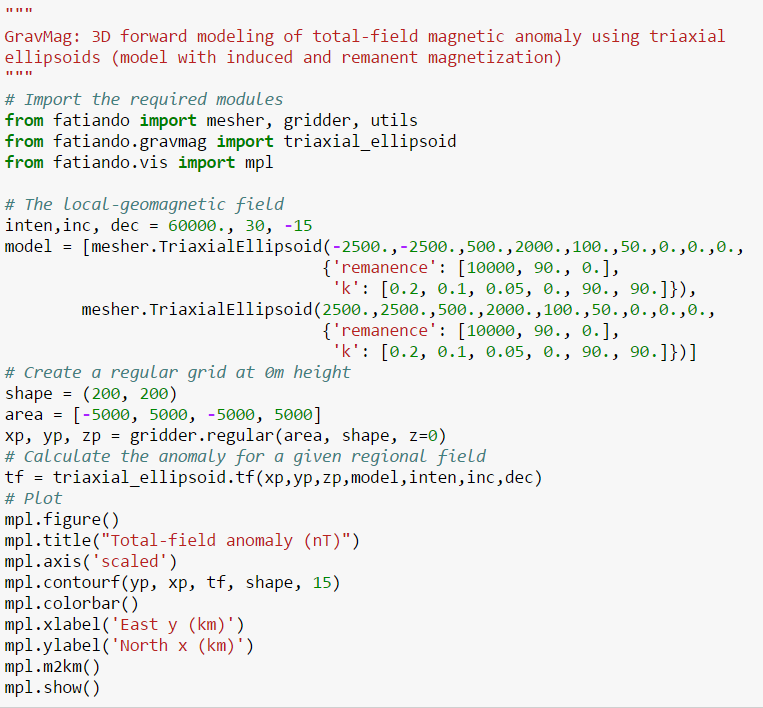
\includegraphics[width=16 cm,height=17 cm]{figures/Cookbook_Triaxial}
	\caption[Exemplo de \textit{script} para gerar um modelo elipsoidal triaxial e calcular a anomalia de campo total $\Delta T (\mathbf{r})$ (Eq. \ref{eq:delta-T-tilde-approx}).]{Exemplo de \textit{script} para gerar um modelo elipsoidal triaxial e calcular a anomalia de campo total $\Delta T (\mathbf{r})$ (Eq. \ref{eq:delta-T-tilde-approx}).}
	\label{fig:Cookbook_Triaxial}
\end{figure}

\begin{figure}[hbt!]
	\centering 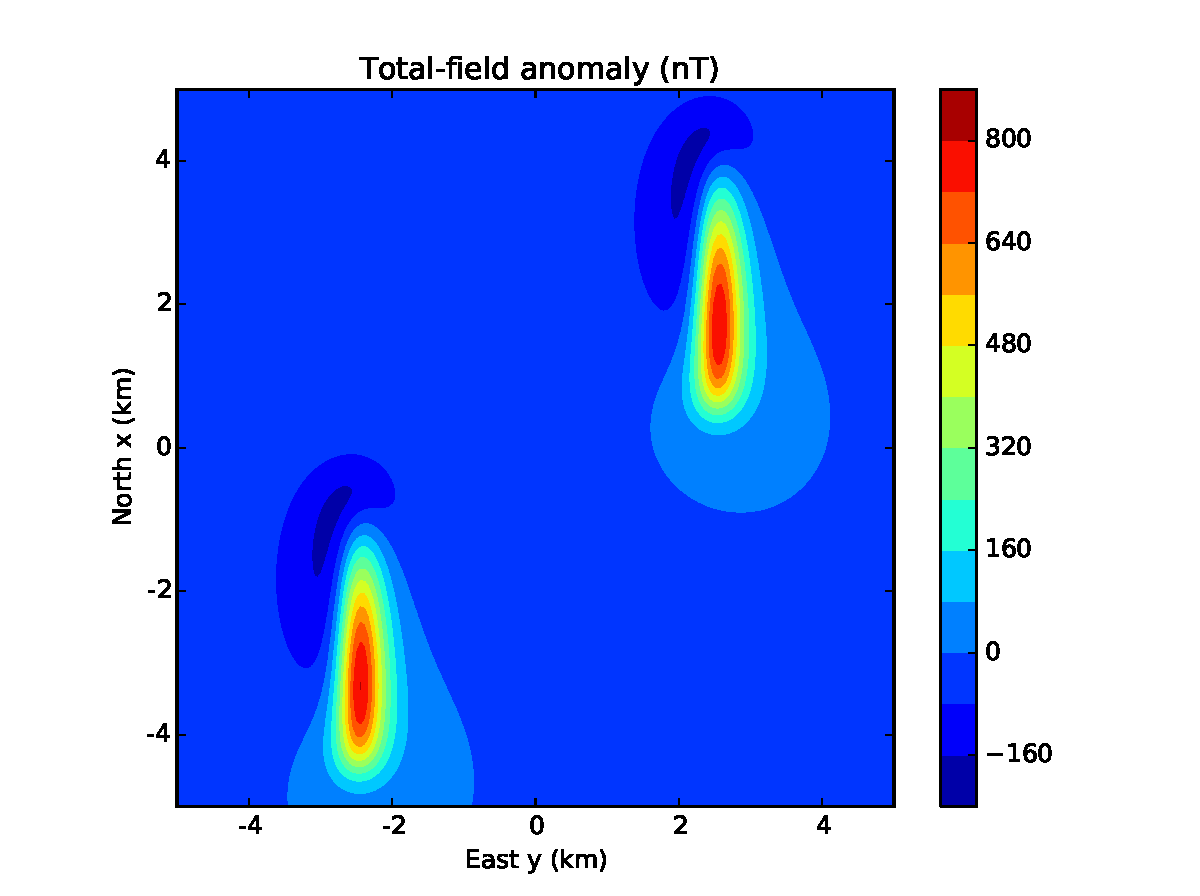
\includegraphics[width=16 cm,height=12 cm]{figures/anomaly_exemplo}
	\caption[Anomalia de campo total $\Delta T (\mathbf{r})$ (Eq. \ref{eq:delta-T-tilde-approx}) produzida pelo código da Fig. \ref{fig:Cookbook_Triaxial}.]{Anomalia de campo total $\Delta T (\mathbf{r})$ (Eq. \ref{eq:delta-T-tilde-approx}) produzida pelo código da Fig. \ref{fig:Cookbook_Triaxial}.}
	\label{fig:anomaly_exemplo}
\end{figure}

\begin{figure}[hbt!]
	\centering 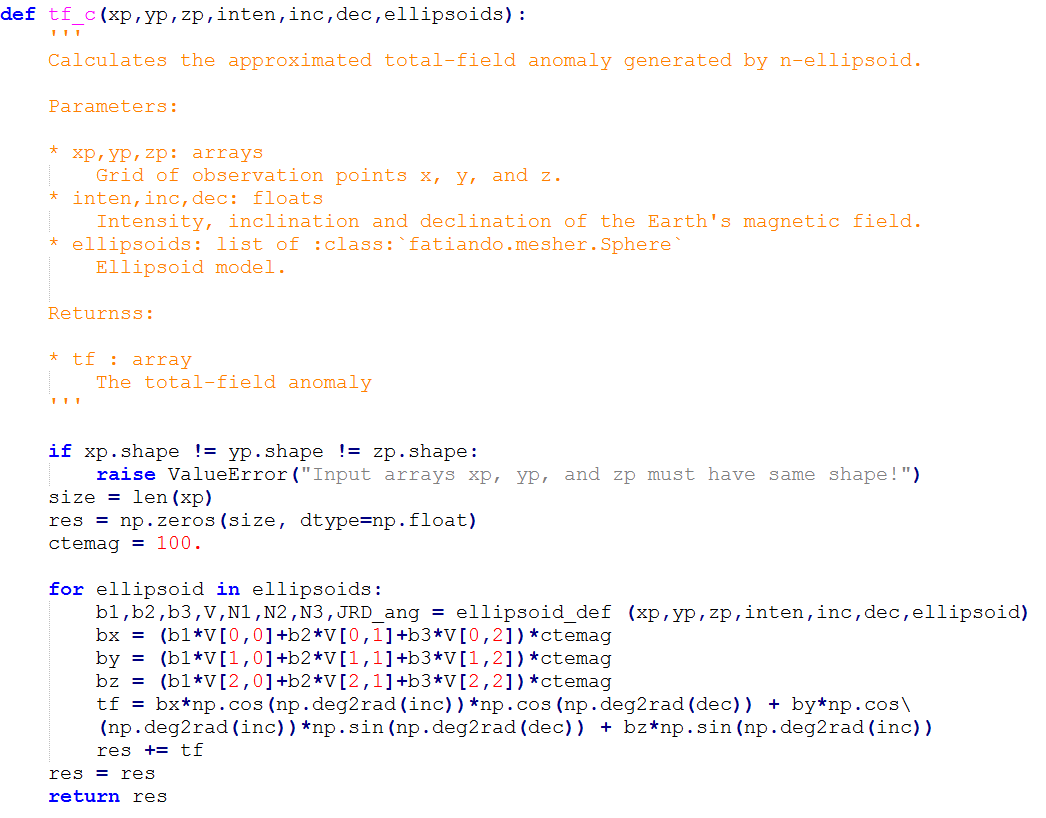
\includegraphics[width=16 cm,height=14 cm]{figures/func_triaxial}
	\caption[Código fonte da rotina \textit{``tf\underline{ }c"} utilizada para calcular a anomalia de campo total $\Delta T (\mathbf{r})$ (Eq.\ref{eq:delta-T-tilde-approx}) produzida pelo modelo elipsoidal definido na Fig. \ref{fig:Cookbook_Triaxial}. Esta rotina utiliza outra rotinas que também foram desenvolvidas neste trabalho como parte do módulo \textit{ellipsoid\underline{ }triaxial} (Fig. \ref{fig:Cookbook_Triaxial}).]{Código fonte da rotina \textit{``tf\underline{ }c"} utilizada para calcular a anomalia de campo total $\Delta T (\mathbf{r})$ (Eq.\ref{eq:delta-T-tilde-approx}) produzida pelo modelo elipsoidal definido na Fig. \ref{fig:Cookbook_Triaxial}. Esta rotina utiliza outra rotinas que também foram desenvolvidas neste trabalho como parte do módulo \textit{ellipsoid\underline{ }triaxial} (Fig. \ref{fig:Cookbook_Triaxial}).}
	\label{fig:func_triaxial}
\end{figure}

\begin{figure}[hbt!]
	\centering 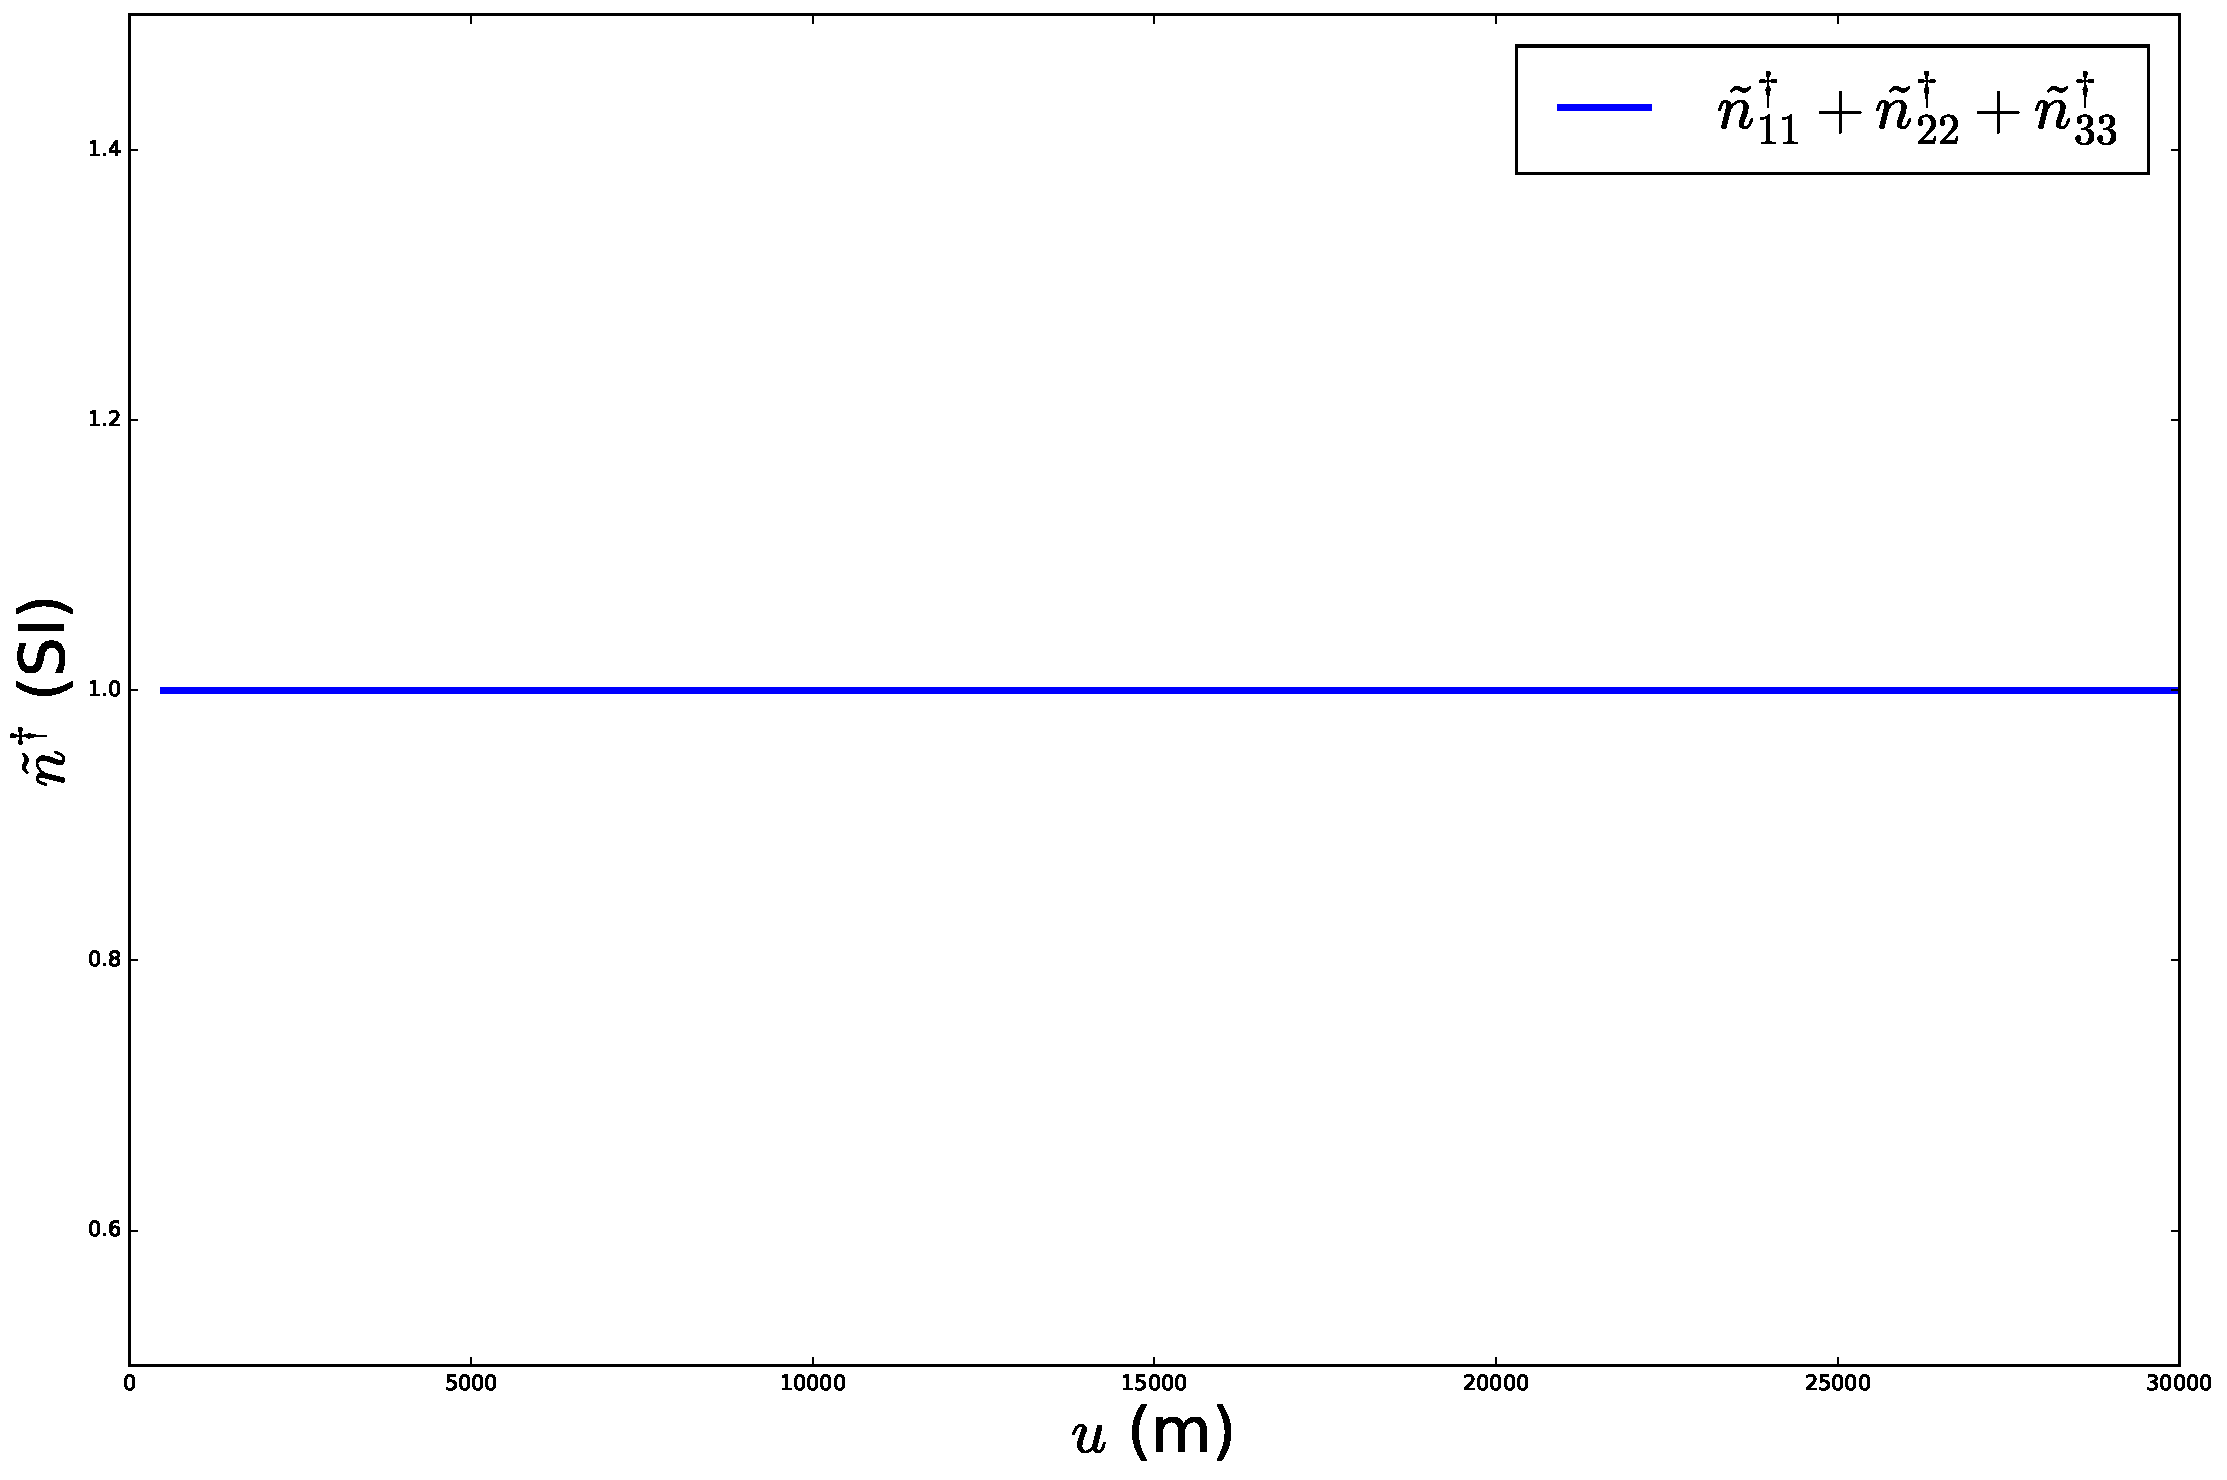
\includegraphics[width=15 cm,height=10 cm]{figures/test_n_soma}
	\caption[Validação dos fatores de desmagnetização. Foram gerados 200 elipsoides triaxiais com semi-eixos $a = a_0 +u, \, b = b_0+u$ e $c = c_0+u$, em que $a_0=500$ m, $b_0=100$ m, $c_0=50$ m e $500  \le u \le 30000$ m. A figura mostra a soma dos fatores de desmagnetização $\tilde{n}^{\dagger}_{11}$, $\tilde{n}^{\dagger}_{22}$ e $\tilde{n}^{\dagger}_{33}$ (Eqs. \ref{eq:n-tilde-dagger-11-triaxial}, \ref{eq:n-tilde-dagger-22-triaxial} e \ref{eq:n-tilde-dagger-33-triaxial}), que está representada pela linha azul, que é igual à 1 (um), independente do tamanho dos eixos e do tipo de elipsoide.]{Validação dos fatores de desmagnetização. Foram gerados 200 elipsoides triaxiais com semi-eixos $a = a_0 +u, \, b = b_0+u$ e $c = c_0+u$, em que $a_0=500$ m, $b_0=100$ m, $c_0=50$ m e $500  \le u \le 30000$ m. A figura mostra a soma dos fatores de desmagnetização $\tilde{n}^{\dagger}_{11}$, $\tilde{n}^{\dagger}_{22}$ e $\tilde{n}^{\dagger}_{33}$ (Eqs. \ref{eq:n-tilde-dagger-11-triaxial}, \ref{eq:n-tilde-dagger-22-triaxial} e \ref{eq:n-tilde-dagger-33-triaxial}), que está representada pela linha azul, que é igual à 1 (um), independente do tamanho dos eixos e do tipo de elipsoide.}
	\label{fig:teste_n_soma}
\end{figure}

  \chapter{Simulações Numéricas e Discussões}

Diversas simulações com o código foram aplicadas, com o intuito de confirmar a resposta obtida pelo código, verificar a  as aplicações e levantar discussões à cerca do modelo elipsoidal.

\section{Modelos elipsoidais}

A implementação computacional feita, nos permite modelar elipsoides triaxiais, prolatos e oblatos para calcular o campo magnético gerado por estes corpos e a anomalia de campo total aproximada (Eqs. \ref{eq:delta-H} e \ref{eq:delta-T-tilde-approx}). Na Figura \ref{fig:triaxial} temos a resposta do campo magnético gerado por um elipsoide triaxial com parâmetros conforme dado na Tabela \ref{tab:triaxial}.

\begin{table}[h]
	\begin{center}
		\begin{tabular}{|l|c|c|}
			\hline
			\textbf{Parâmetro}  & \textbf{Valor}  & \textbf{Unidade} \\
			\hline 
			a, b, c   & 150, 100, 75 & m\\
			\hline
			Azimute   & $0$ & º\\
			\hline
			$\delta$ & $0$ & º\\
			\hline
			$\gamma$ & $0$  & º\\
			\hline
			xc   & 0  & m\\
			\hline          
			yc   & 0  & m\\
			\hline                
			zc   & 1000 & m\\
			\hline
			$J_{NRM}$*  & 100, $25^o$, $40^o$  & A/m\\
			\hline
			F*    & 60000, $50^o$, $20^o$ & nT\\
			\hline
			k1, k2, k3   & 0.1, 0.1, 0.1  & SI\\
			\hline
			Orientações k**   & $0$, $90$, $90$  & º\\
			\hline
		\end{tabular}
		\caption{Parâmetros do elipsoide triaxial modelado. *Valores de intensidade, inclinação e declinação respectivamente. **Ângulo de azimute, $\delta$ e $\gamma$, respectivamente, para as orientações da susceptibilidade.}
	\end{center}
	\label{tab:triaxial}
\end{table}

\begin{figure}[hbt!]
	\centering 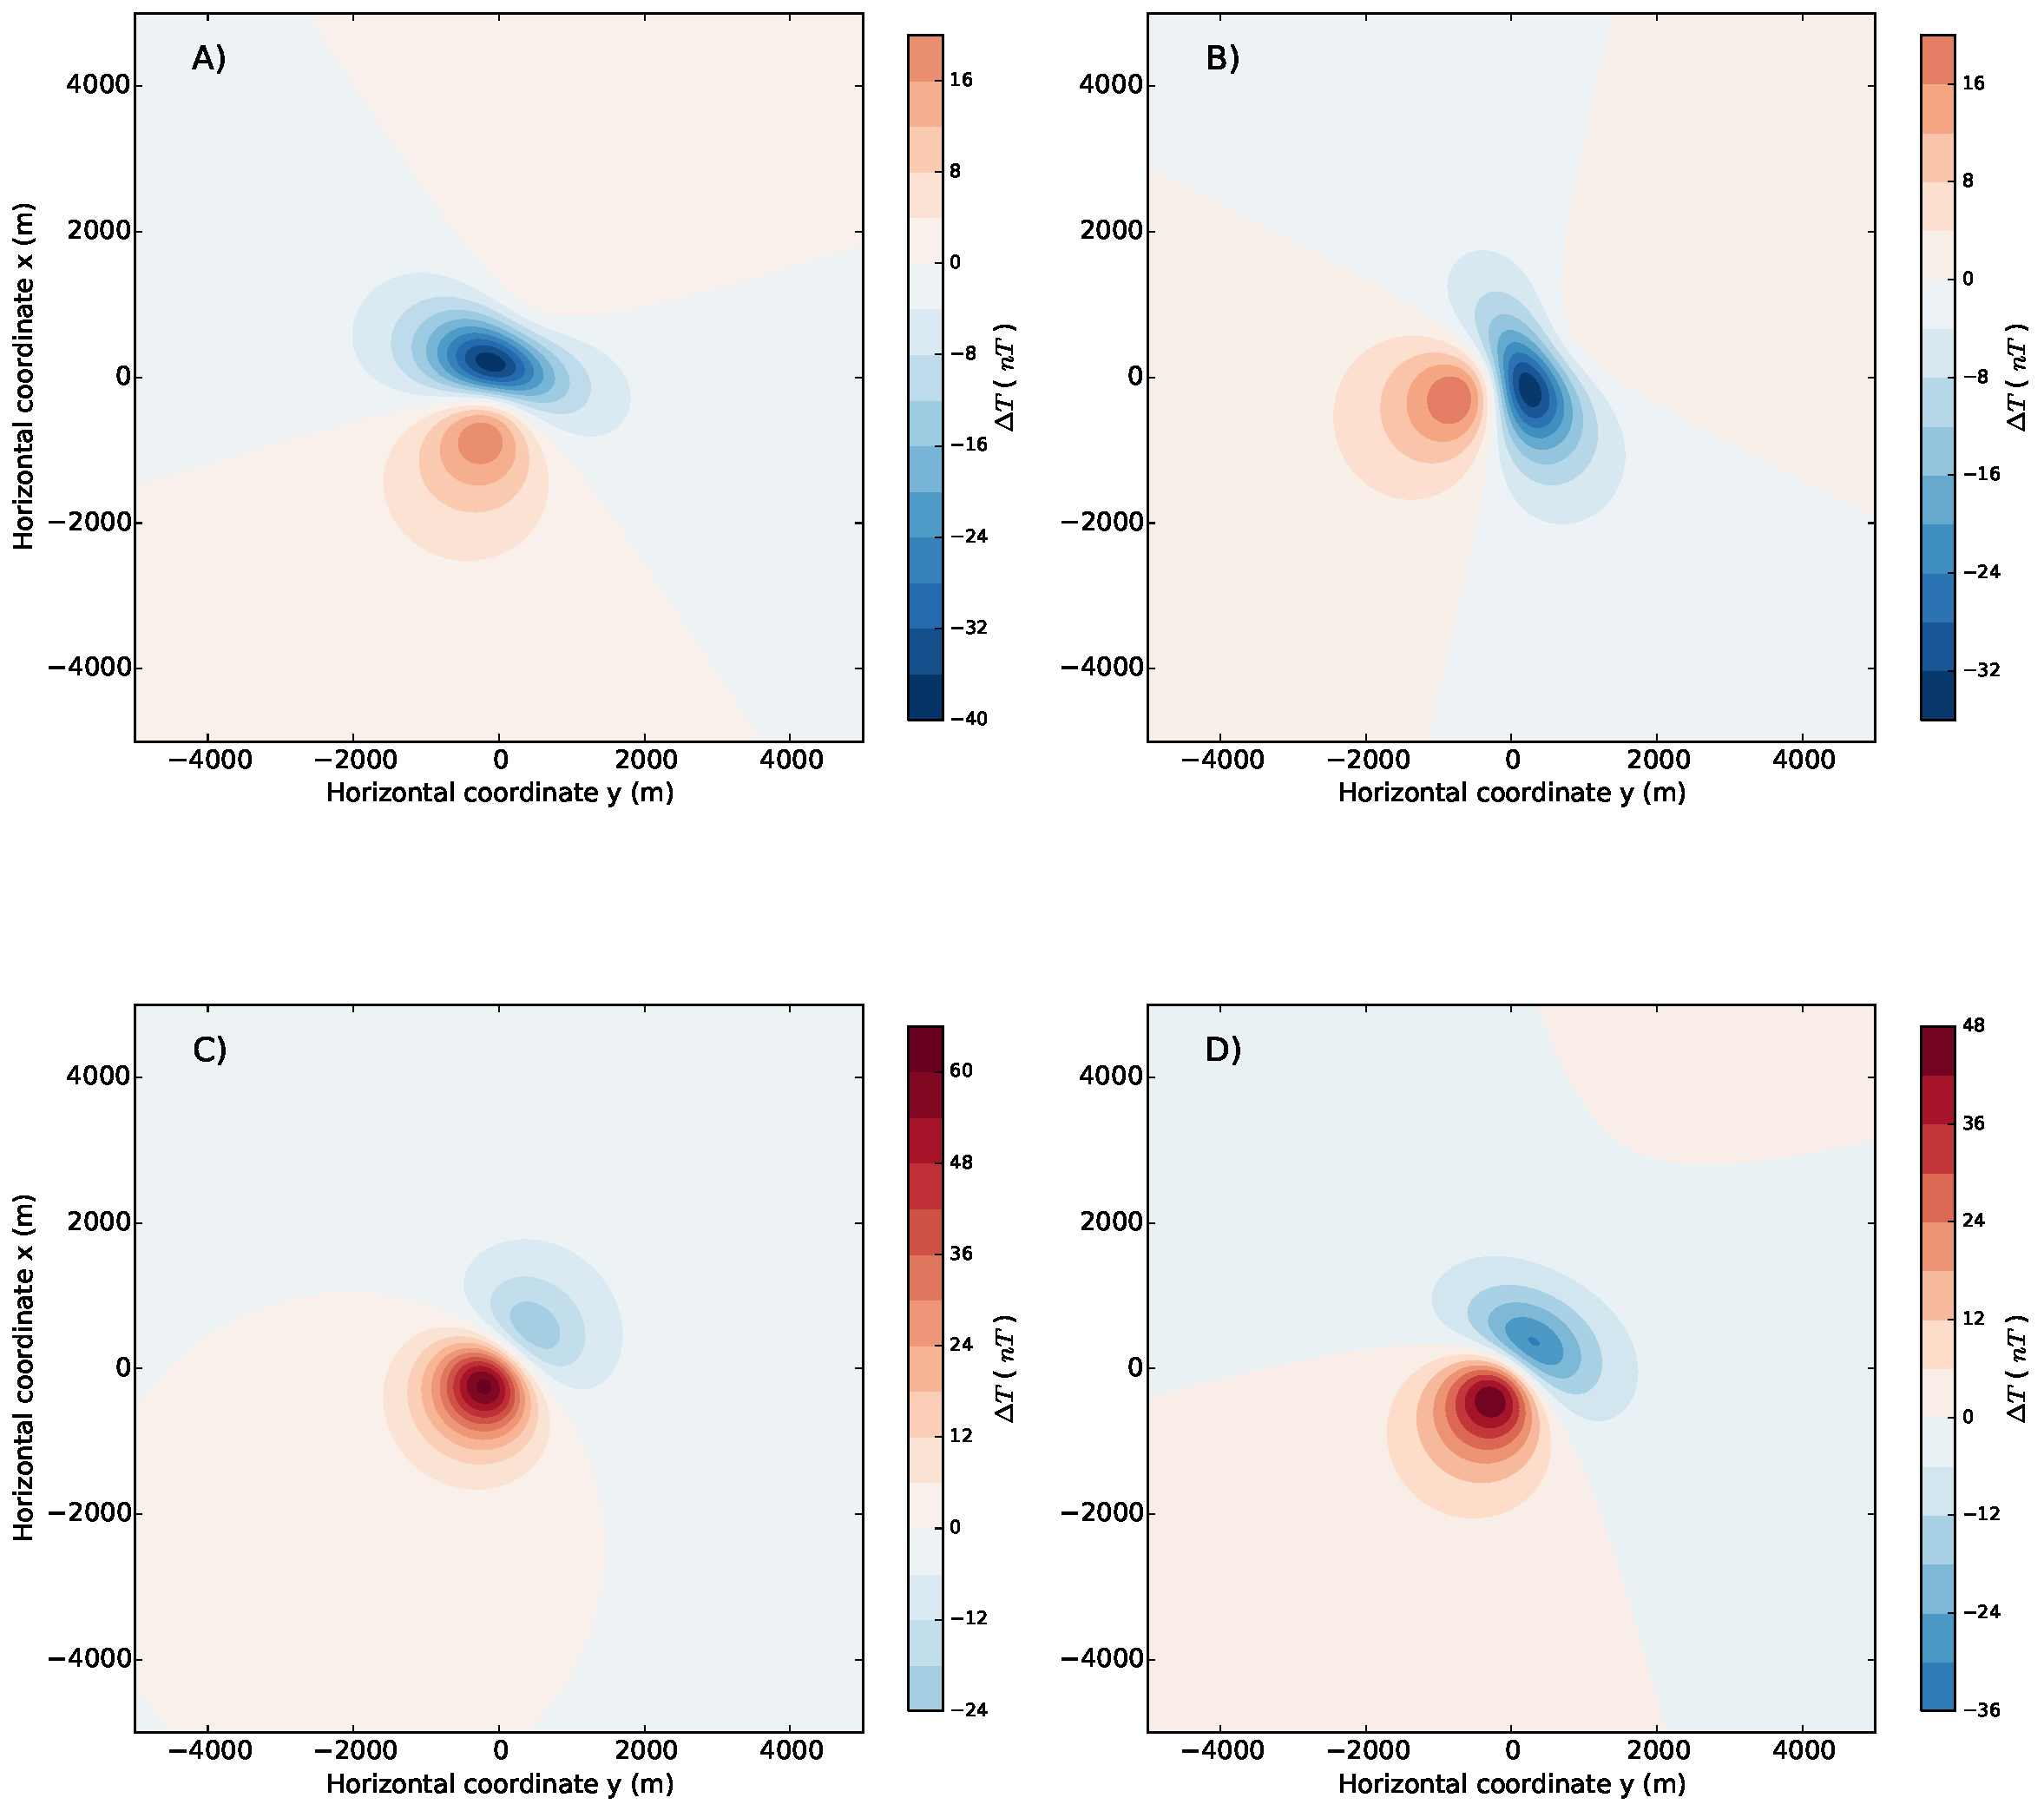
\includegraphics[width=16cm,height=16cm]{figures/ellipsoid_triaxial}
	\caption[As componentes do campo magnético gerado por um elipsoide triaxial e a anomalia de campo total aproximada.]{As componentes 
		do campo magnético gerado por um elipsoide triaxial de parâmetros conforme a tabela \ref{tab:triaxial} e a anomalia de campo total aproximada. Em A) a componente Bx do campo, em B) a componente By, em C) a componente Bz e em D) a anomalia de campo total aproximada.}
	\label{fig:triaxial}
\end{figure}

Uma malha de de $40000$ pontos foi criada ($200$x$200$) para os cálculos das três componentes e da anomalia de campo total aproximada em todas as simulações.

Na Figura \ref{fig:prolate} temos as três componentes do campo magnético gerado por um elipsoide triaxial com os parâmetros da Tabela 4.2.

Na Figura \ref{fig:oblate} temos as três componentes do campo magnético gerado por um elipsoide triaxial com os parâmetros da Tabela 4.3.
\\\\\\

\begin{table}[h!]
	\begin{center}
		\begin{tabular}{|l|c|c|}
			\hline
			\textbf{Parâmetro}  & \textbf{Valor}  & \textbf{Unidade} \\
			\hline 
			a,b   & 200, 100 & m\\
			\hline
			Azimute   & $45$ & º\\
			\hline
			$\delta$    & $0$ & º\\
			\hline
			$\gamma$   & $0$  & º\\
			\hline
			xc   & 0  & m\\
			\hline          
			yc   & 0  & m\\
			\hline                
			zc   & 1000  & m\\
			\hline
			$J_{NRM}$*  & 100, $90^o$, $0^o$ & A/m\\
			\hline
			F*    & 60000, $50^o$, $20^o$ & nT\\
			\hline
			k1, k2, k3   & 0.1, 0.1, 0.1  & SI\\
			\hline
			Orientações k**   & $0$, $90$, $90$  & º\\
			\hline
			
		\end{tabular}
		\caption{Parâmetros do elipsoide prolato modelado. *Valores de intensidade, inclinação e declinação respectivamente. **Ângulo de azimute, $\delta$ e $\gamma$, respectivamente, para as orientações da susceptibilidade.}
	\end{center}
	\label{tab:prolato}
\end{table}

\begin{table}[h!]
	\begin{center}
		\begin{tabular}{lc}
		
			 &  \\
			 & \\
			 & \\
			 & \\
			& \\
			& \\ 
			& \\
			& \\
			& \\ 
			& \\
\end{tabular}
\end{center}
\end{table}

\begin{table}[h!]
	\begin{center}
		\begin{tabular}{|l|c|c|}
			\hline
			\textbf{Parâmetro}  & \textbf{Valor} & \textbf{Unidade} \\
			\hline 
			a, b  & 100, 200 & m \\
			\hline
			Azimute   & $45$ & º\\
			\hline
			$\delta$    & $0$ & º\\
			\hline
			$\gamma$   & $0$  & º\\
			\hline
			xc   & 0  & m\\
			\hline          
			yc   & 0  & m\\
			\hline                
			zc   & 1000  & m\\
			\hline
			$J_{NRM}$*  & 100, $90^o$, $0^o$  & A/m\\
			\hline
			F*    & 60000, $50^o$, $20^o$ & nT\\
			\hline
			k1, k2, k3   & 0.1, 0.1, 0.1  & SI\\
			\hline
			Orientações k**   & $0$, $90$, $90$  & º\\
			\hline
		\end{tabular}
		\caption{Parâmetros do elipsoide oblato modelado. *Valores de intensidade, inclinação e declinação respectivamente. **Ângulo de azimute, $\delta$ e $\gamma$, respectivamente, para as orientações da susceptibilidade.}
	\end{center}
	\label{tab:oblate}
\end{table}

\begin{figure}[hbt!]
	\centering 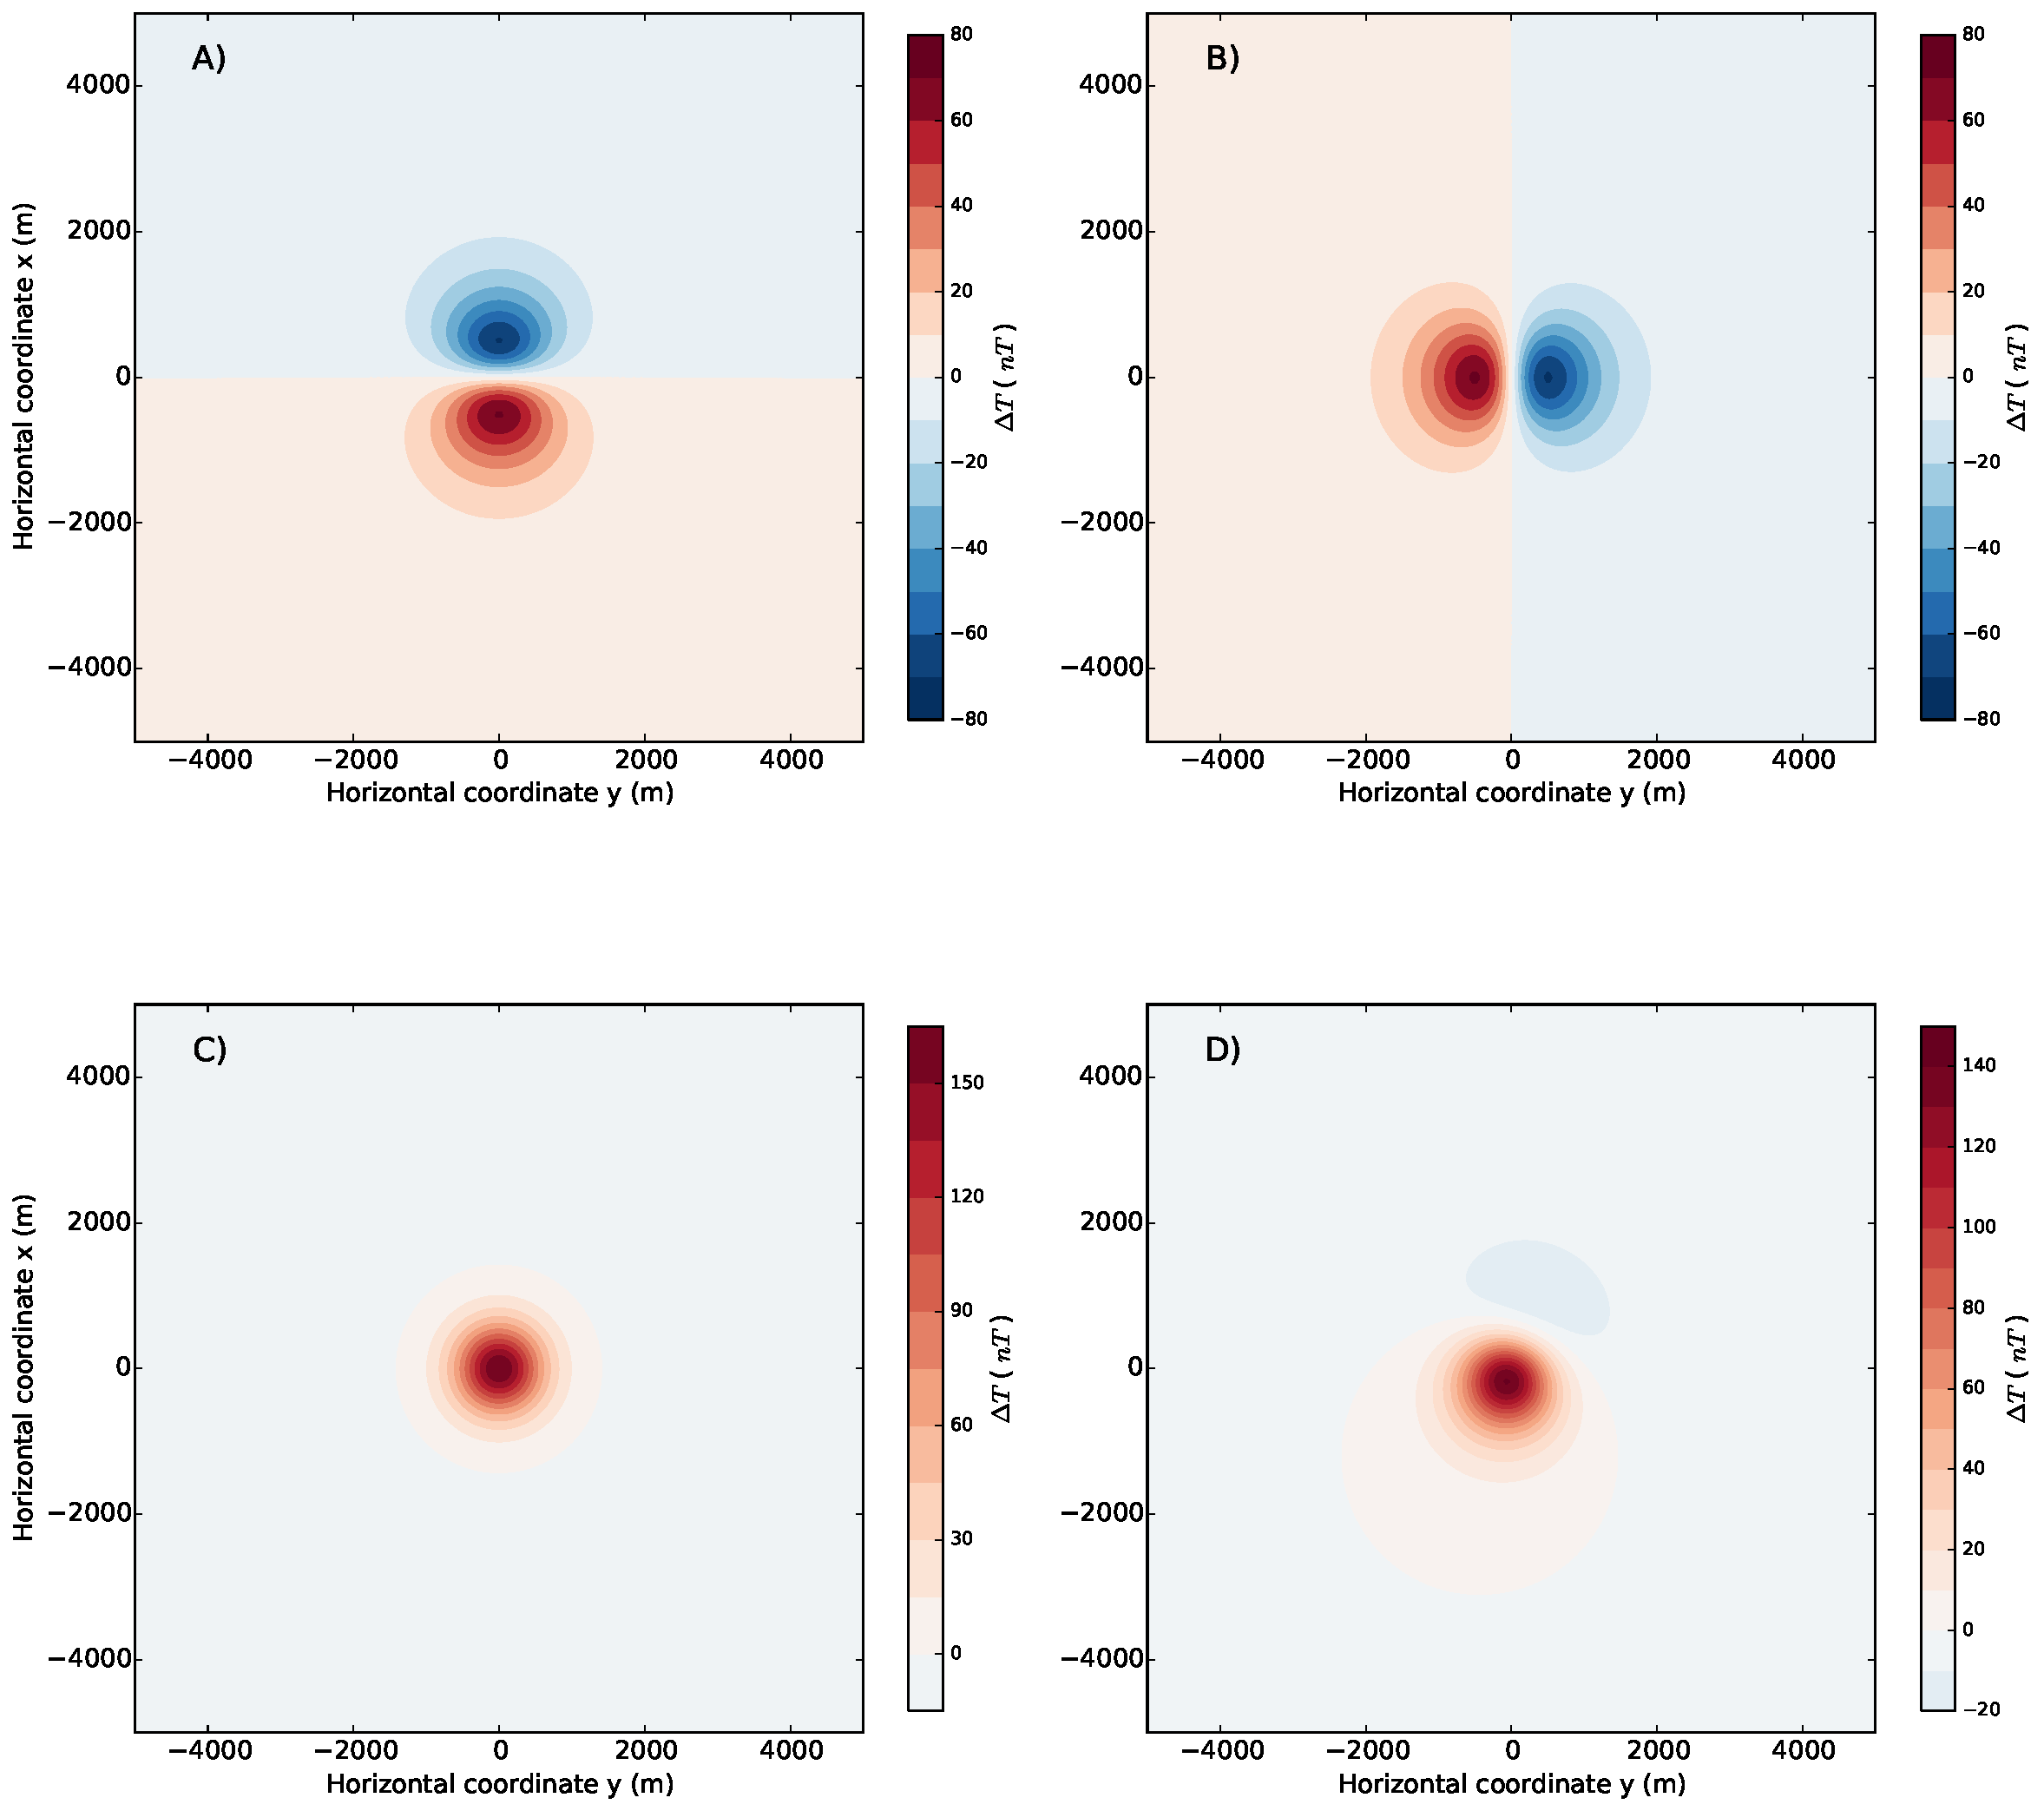
\includegraphics[width=16cm,height=16cm]{figures/ellipsoid_prolate}
	\caption[As componentes do campo magnético gerado por um elipsoide prolato e a anomalia de campo total aproximada.]{As componentes 
		do campo magnético gerado por um elipsoide prolato de parâmetros conforme a tabela 4.2 e a anomalia de campo total aproximada. Em A) a componente Bx do campo, em B) a componente By, em C) a componente Bz e em D) a anomalia de campo total aproximada.}
	\label{fig:prolate}
\end{figure}

\begin{table}[h!]
	\begin{center}
		\begin{tabular}{lc}
			
			&  \\
			& \\
			& \\
			& \\
			& \\
			& \\ 
			& \\
			& \\
		\end{tabular}
	\end{center}
\end{table}

\begin{figure}[hbt!]
	\centering 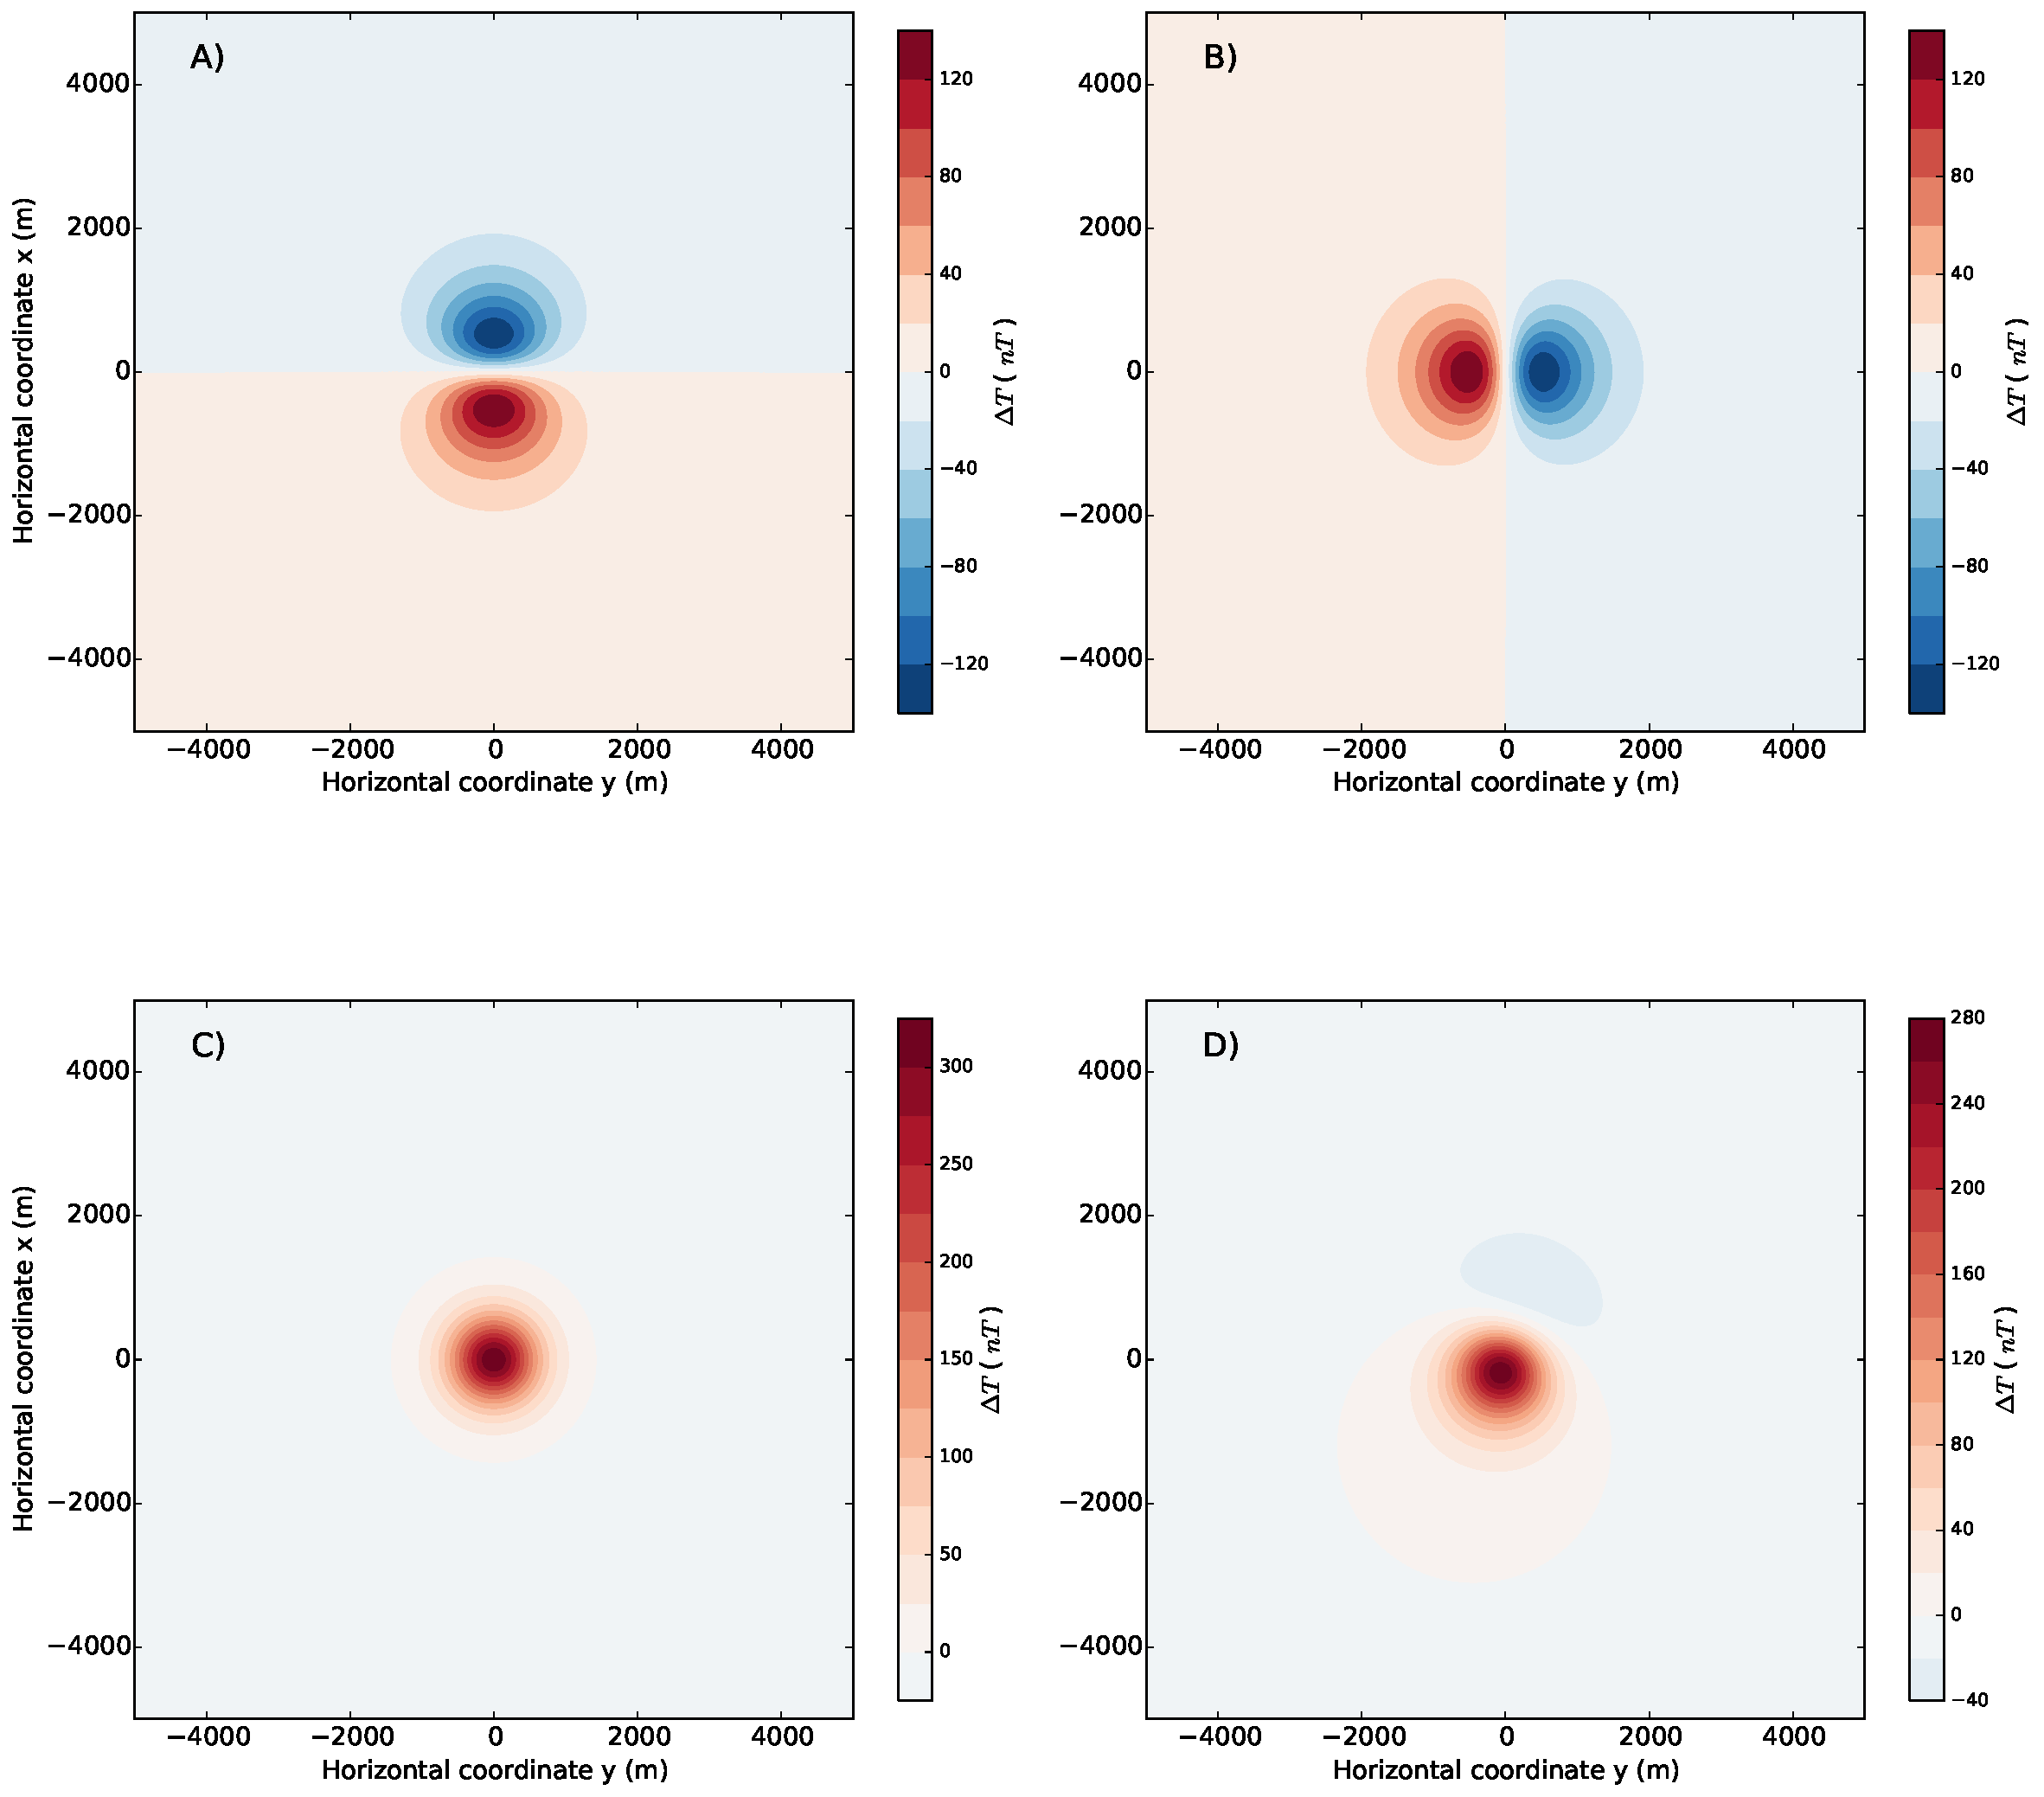
\includegraphics[width=16cm,height=16cm]{figures/ellipsoid_oblate}
	\caption[As componentes do campo magnético gerado por um elipsoide oblato e a anomalia de campo total aproximada.]{As componentes 
		do campo magnético gerado por um elipsoide oblato de parâmetros conforme a tabela 4.3 e a anomalia de campo total aproximada. Em A) a componente Bx do campo, em B) a componente By, em C) a componente Bz e em D) a anomalia de campo total aproximada.}
	\label{fig:oblate}
\end{figure}

Já na Figura \ref{fig:ellipsoid_triaxial_multi}, fizemos uma simulação de dois corpos elipsoidais triaxiais sendo modelados dentro da mesma malha, que pode ser feita de forma prática usando a classe elipsoidal, implementada no \textit{mesher} do \textit{Fatiando a Terra}. Novamente temos as três componentes do campo magnético gerado pelos corpos com os parâmetros da Tabela 4.4.

\begin{table}[h!]
	\begin{center}
		\begin{tabular}{lc}
			
			&  \\
			&  \\
			&  \\
			&  \\
		\end{tabular}
	\end{center}
\end{table}

\begin{table}[h!]
	\begin{center}
		\begin{tabular}{|l|c|c|}
			\hline
			\textbf{Parâmetro}  & \textbf{Valor}  & \textbf{Unidade}\\
			\hline 
			a, b, c   & 150, 100, 75 & m\\
			\hline
			Azimute   & $0$ & º\\
			\hline
			$\delta$    & $0$ & º\\
			\hline
			$\gamma$   & $0$  & º\\
			\hline
			xc   & -2500  & m\\
			\hline          
			yc   & -2500  & m\\
			\hline                
			zc   & 1000  & m\\
			\hline
			$J_{NRM}$*  & 100, $25^o$, $40^o$  & A/m\\
			\hline
			k1, k2, k3   & 0.1, 0.1, 0.1  & SI\\
			\hline
			Orientações k**   & $0$, $90$, $90$  & º\\
			\hline 
			a$_2$, b$_2$, c$_2$   & 200, 120, 60 & m\\
			\hline
			Azimute$_2$   & $0$ & º\\
			\hline
			$\delta_2$    & $0$ & º\\
			\hline
			$\gamma_2$   & $0$  & º\\
			\hline
			xc$_2$   & 2500  & m\\
			\hline          
			yc$_2$   & 2500  & m\\
			\hline                
			zc$_2$   & 1000  & m\\
			\hline
			$J_{2NRM}$*  & 75, $25^o$, $40^o$  & A/m\\
			\hline
			k1$_2$, k2$_2$, k3$_2$   & 0.1, 0.1, 0.1  & SI\\
			\hline
			Orientações k$_2$**   & $0$, $90$, $90$  & º\\
			\hline
			F*    & 60000, $50^o$, $20^o$ & nT\\
			\hline			
		\end{tabular}
		\caption{Parâmetros dos dois elipsoides triaxiais modelados. O segundo elipsoide é mostrada na tabela pela índice $_2$ nos parâmetros. *Valores de intensidade, inclinação e declinação respectivamente. **Ângulo de azimute, $\delta$ e $\gamma$, respectivamente, para as orientações da susceptibilidade.}
	\end{center}
	\label{tab:ellipsoid_triaxial_multi}
\end{table}

\begin{table}[h!]
	\begin{center}
		\begin{tabular}{lc}
			
			&  \\
			& \\
			& \\
			& \\
			& \\
			& \\ 
			& \\
			& \\
				& \\
				& \\ 
				& \\
		\end{tabular}
	\end{center}
\end{table}

\begin{figure}[hbt!]
	\centering 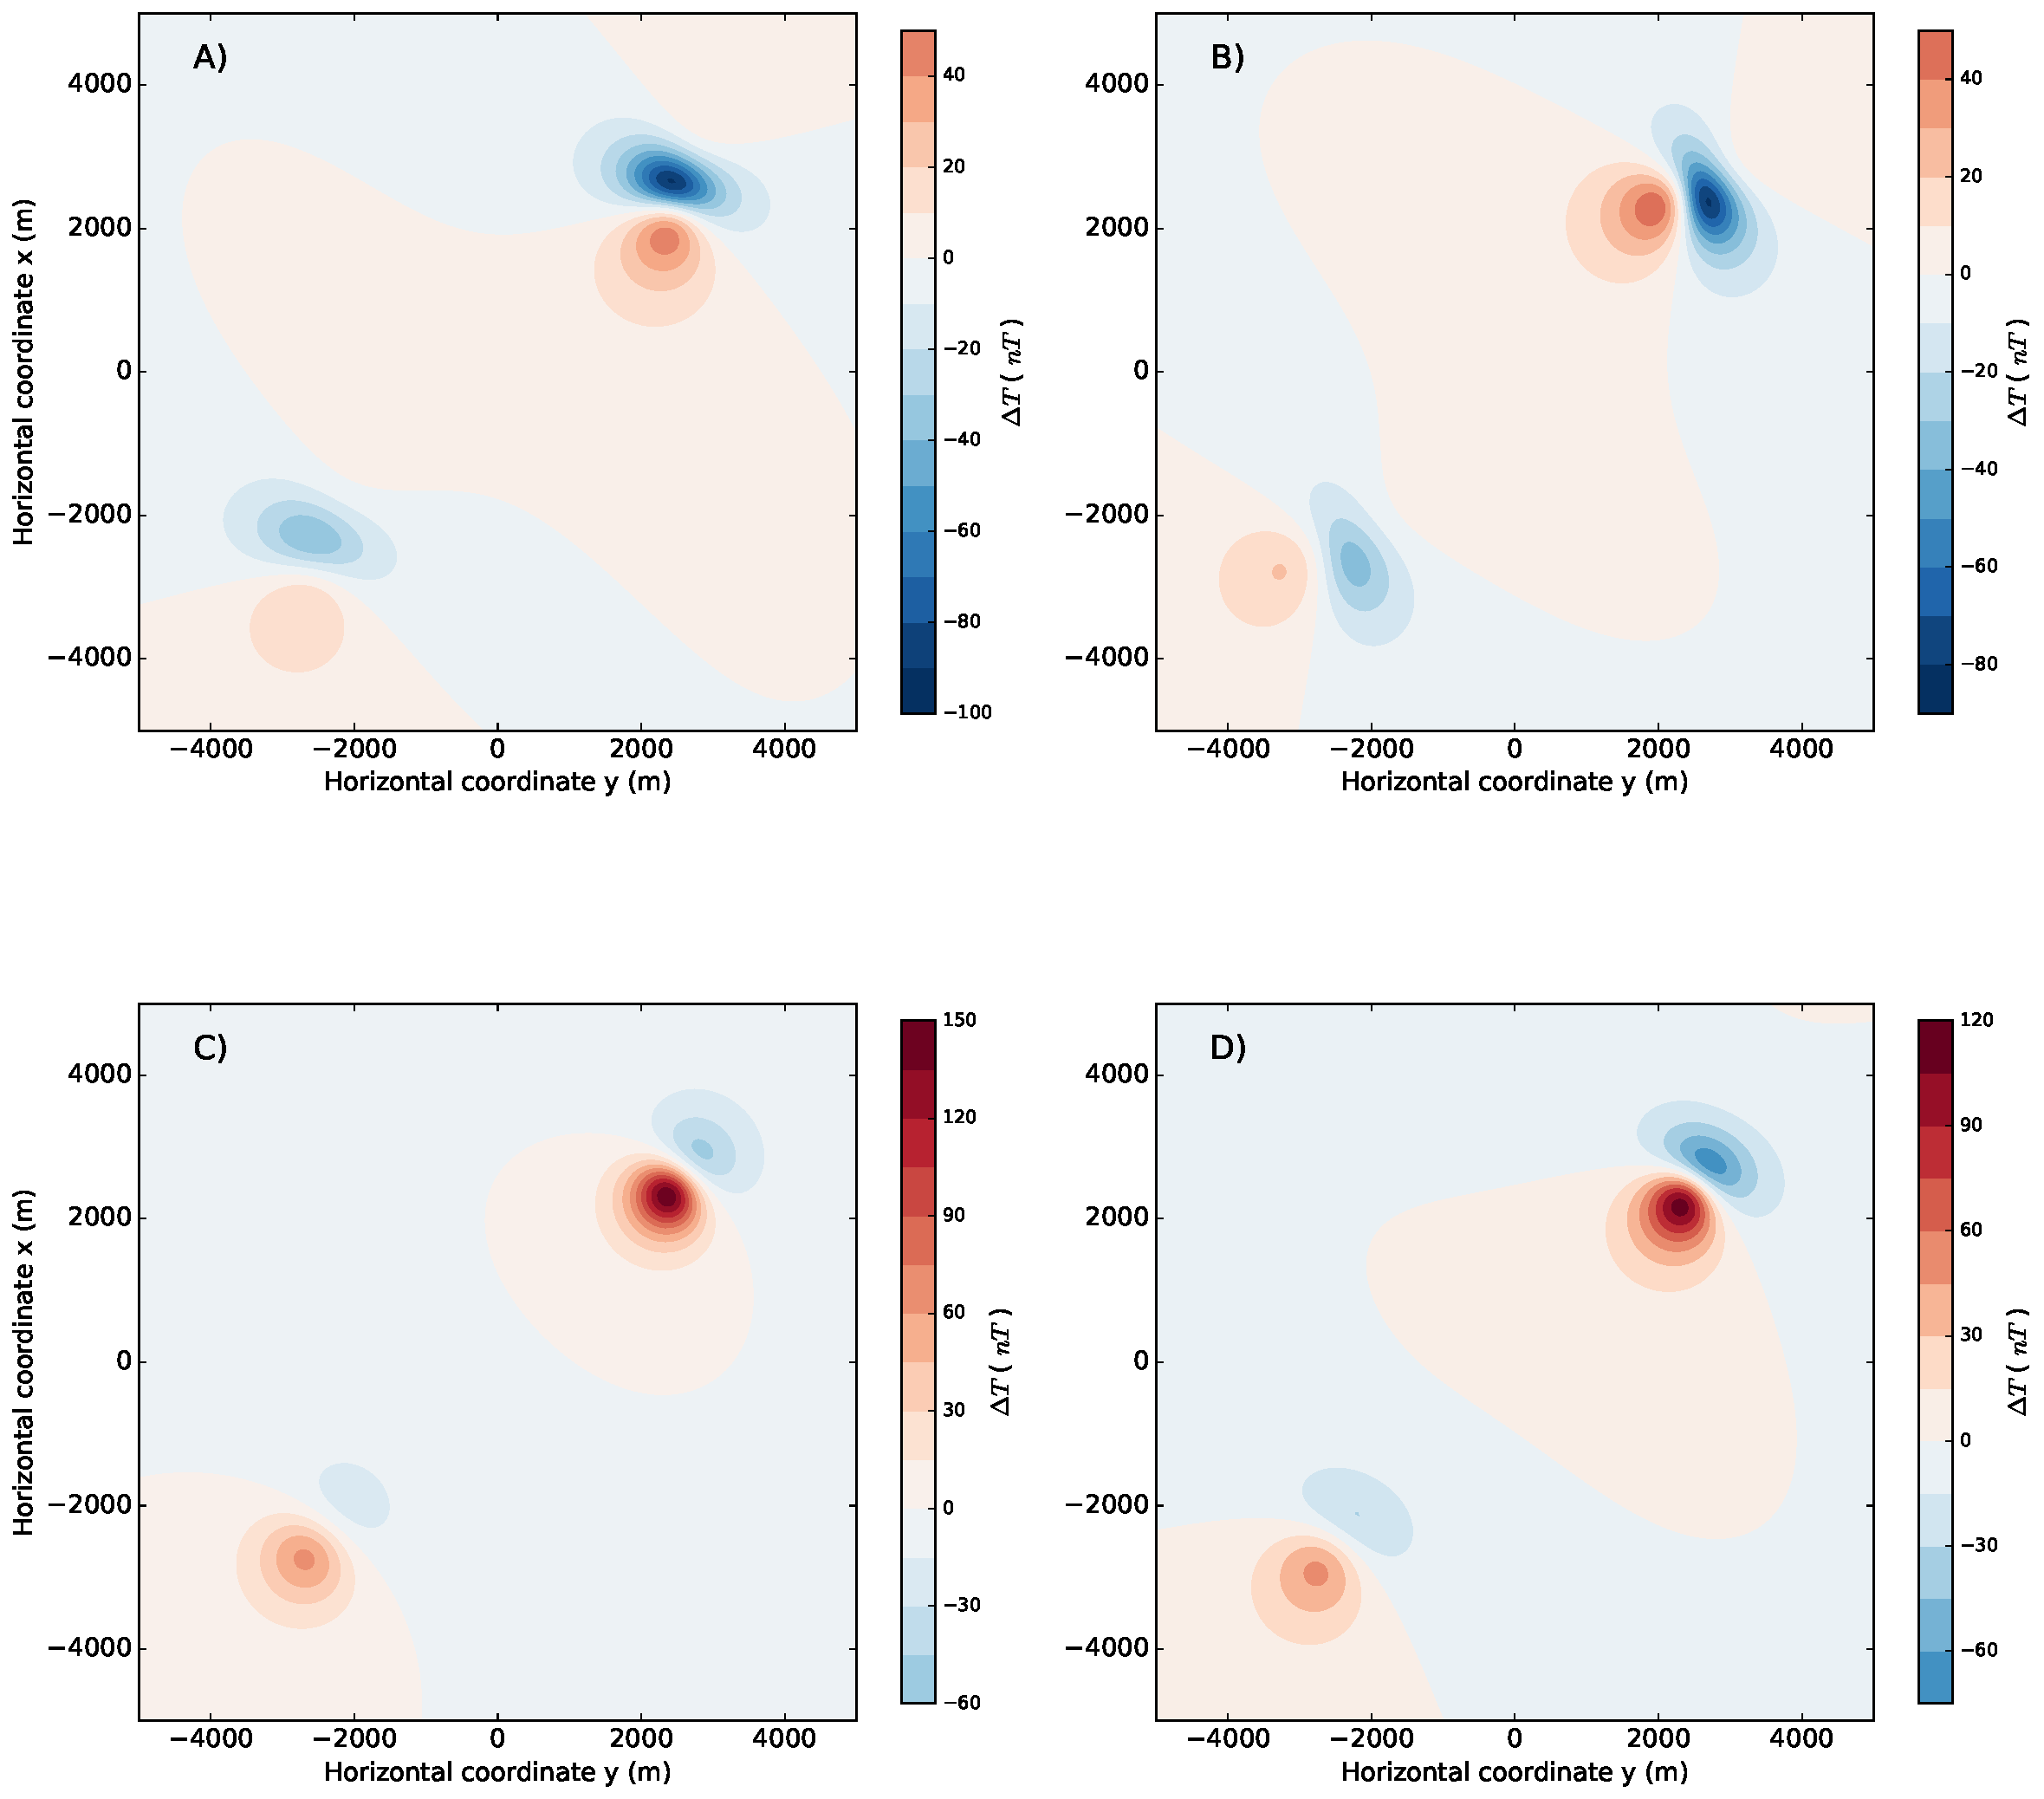
\includegraphics[width=16cm,height=16cm]{figures/ellipsoid_triaxial_multi}
	\caption[As componentes do campo magnético gerado por dois corpos triaxiais e a anomalia de campo total aproximada.]{As componentes 
		do campo magnético gerado pelos elipsoides triaxiais de parâmetros conforme a tabela 4.4 e a anomalia de campo total aproximada. Em A) a componente Bx do campo, em B) a componente By, em C) a componente Bz e em D) a anomalia de campo total aproximada.}
	\label{fig:ellipsoid_triaxial_multi}
\end{figure}

\begin{table}[h!]
	\begin{center}
		\begin{tabular}{lc}
			
			&  \\
			& \\
			& \\
			& \\
			& \\
			& \\ 
			& \\
			& \\
		\end{tabular}
	\end{center}
\end{table}

\section{Elementos do tensor de depolarização}

Os fatores de desmagnetização são importantíssimos para a modelagem de corpos com alta susceptibilidade e dependem apenas da sua forma geométrica, no modelo elipsoidal. 

Na Figura \ref{fig:n_triaxial} observamos o comportamento afastado destes elementos, quando os semi-eixos de elipsoide triaxial possuem tamanhos diferentes, e a tendência de se aproximarem para um mesmo valor quando possuem tamanhos próximos (se aproximando de uma esfera, que possui o valor de $1/3$ no SI para todos os elementos dos fatores de desmagnetização).


\begin{figure}[hbt!]
	\centering 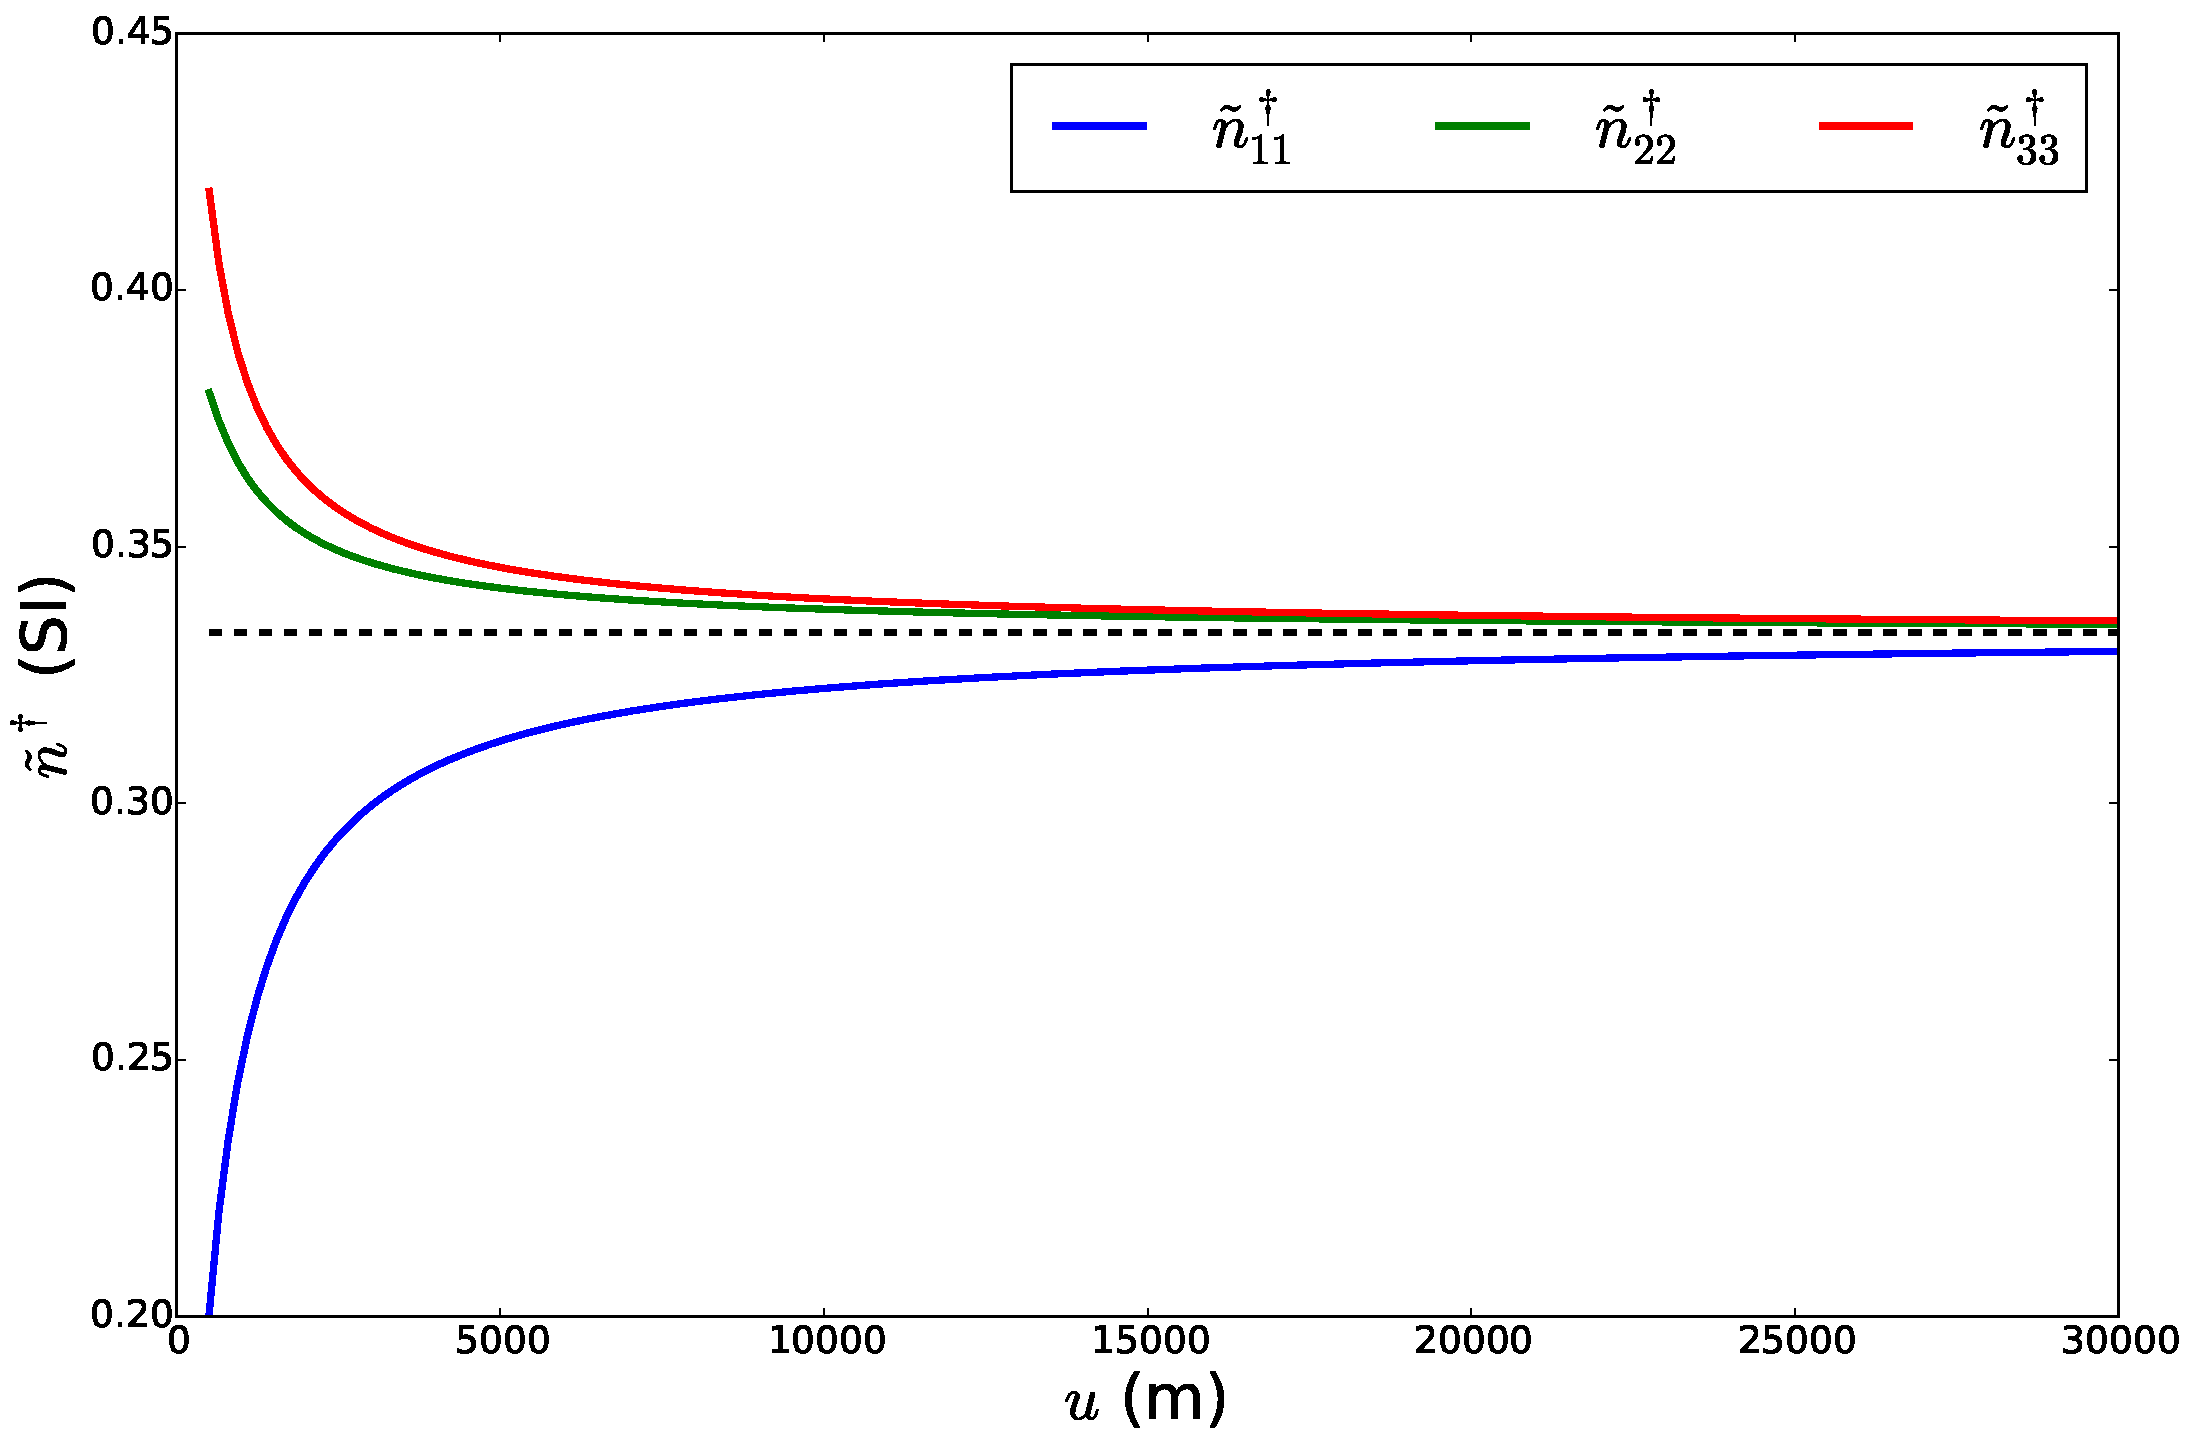
\includegraphics[width=15cm,height=10cm]{figures/test_n_triaxial}
	\caption[Teste dos fatores de desmagnetização para um elipsoide triaxial.]{Teste dos fatores de desmagnetização:
		$\tilde{n}^{\dagger}_{11}$, $\tilde{n}^{\dagger}_{22}$ e $\tilde{n}^{\dagger}_{33}$ 
		para um elipsoide triaxial originalmente com semi-eixos 500, 100 e 50 metros, com um fator $u$ crescente,
		somando, simultaneamente, todos os semi-eixos.}
	\label{fig:n_triaxial}
\end{figure}

Na Figura \ref{fig:n_prolato} observamos o mesmo comportamento no caso triaxial para o caso do elipsoide prolato. Neste gráfico no eixo horizontal é feita a relação entre os semi-eixos $a$ e $b$ ($m$) onde aumenta-se a valor do semi-eixo maior e mantém o semi-eixo menor constante. No começo, quando os semi-eixos estão próximos, os elementos tendem à $1/3$ e se afastam conforme $a$ é muito maior que $b$.
\newpage

\begin{figure}[hbt!]
	\centering 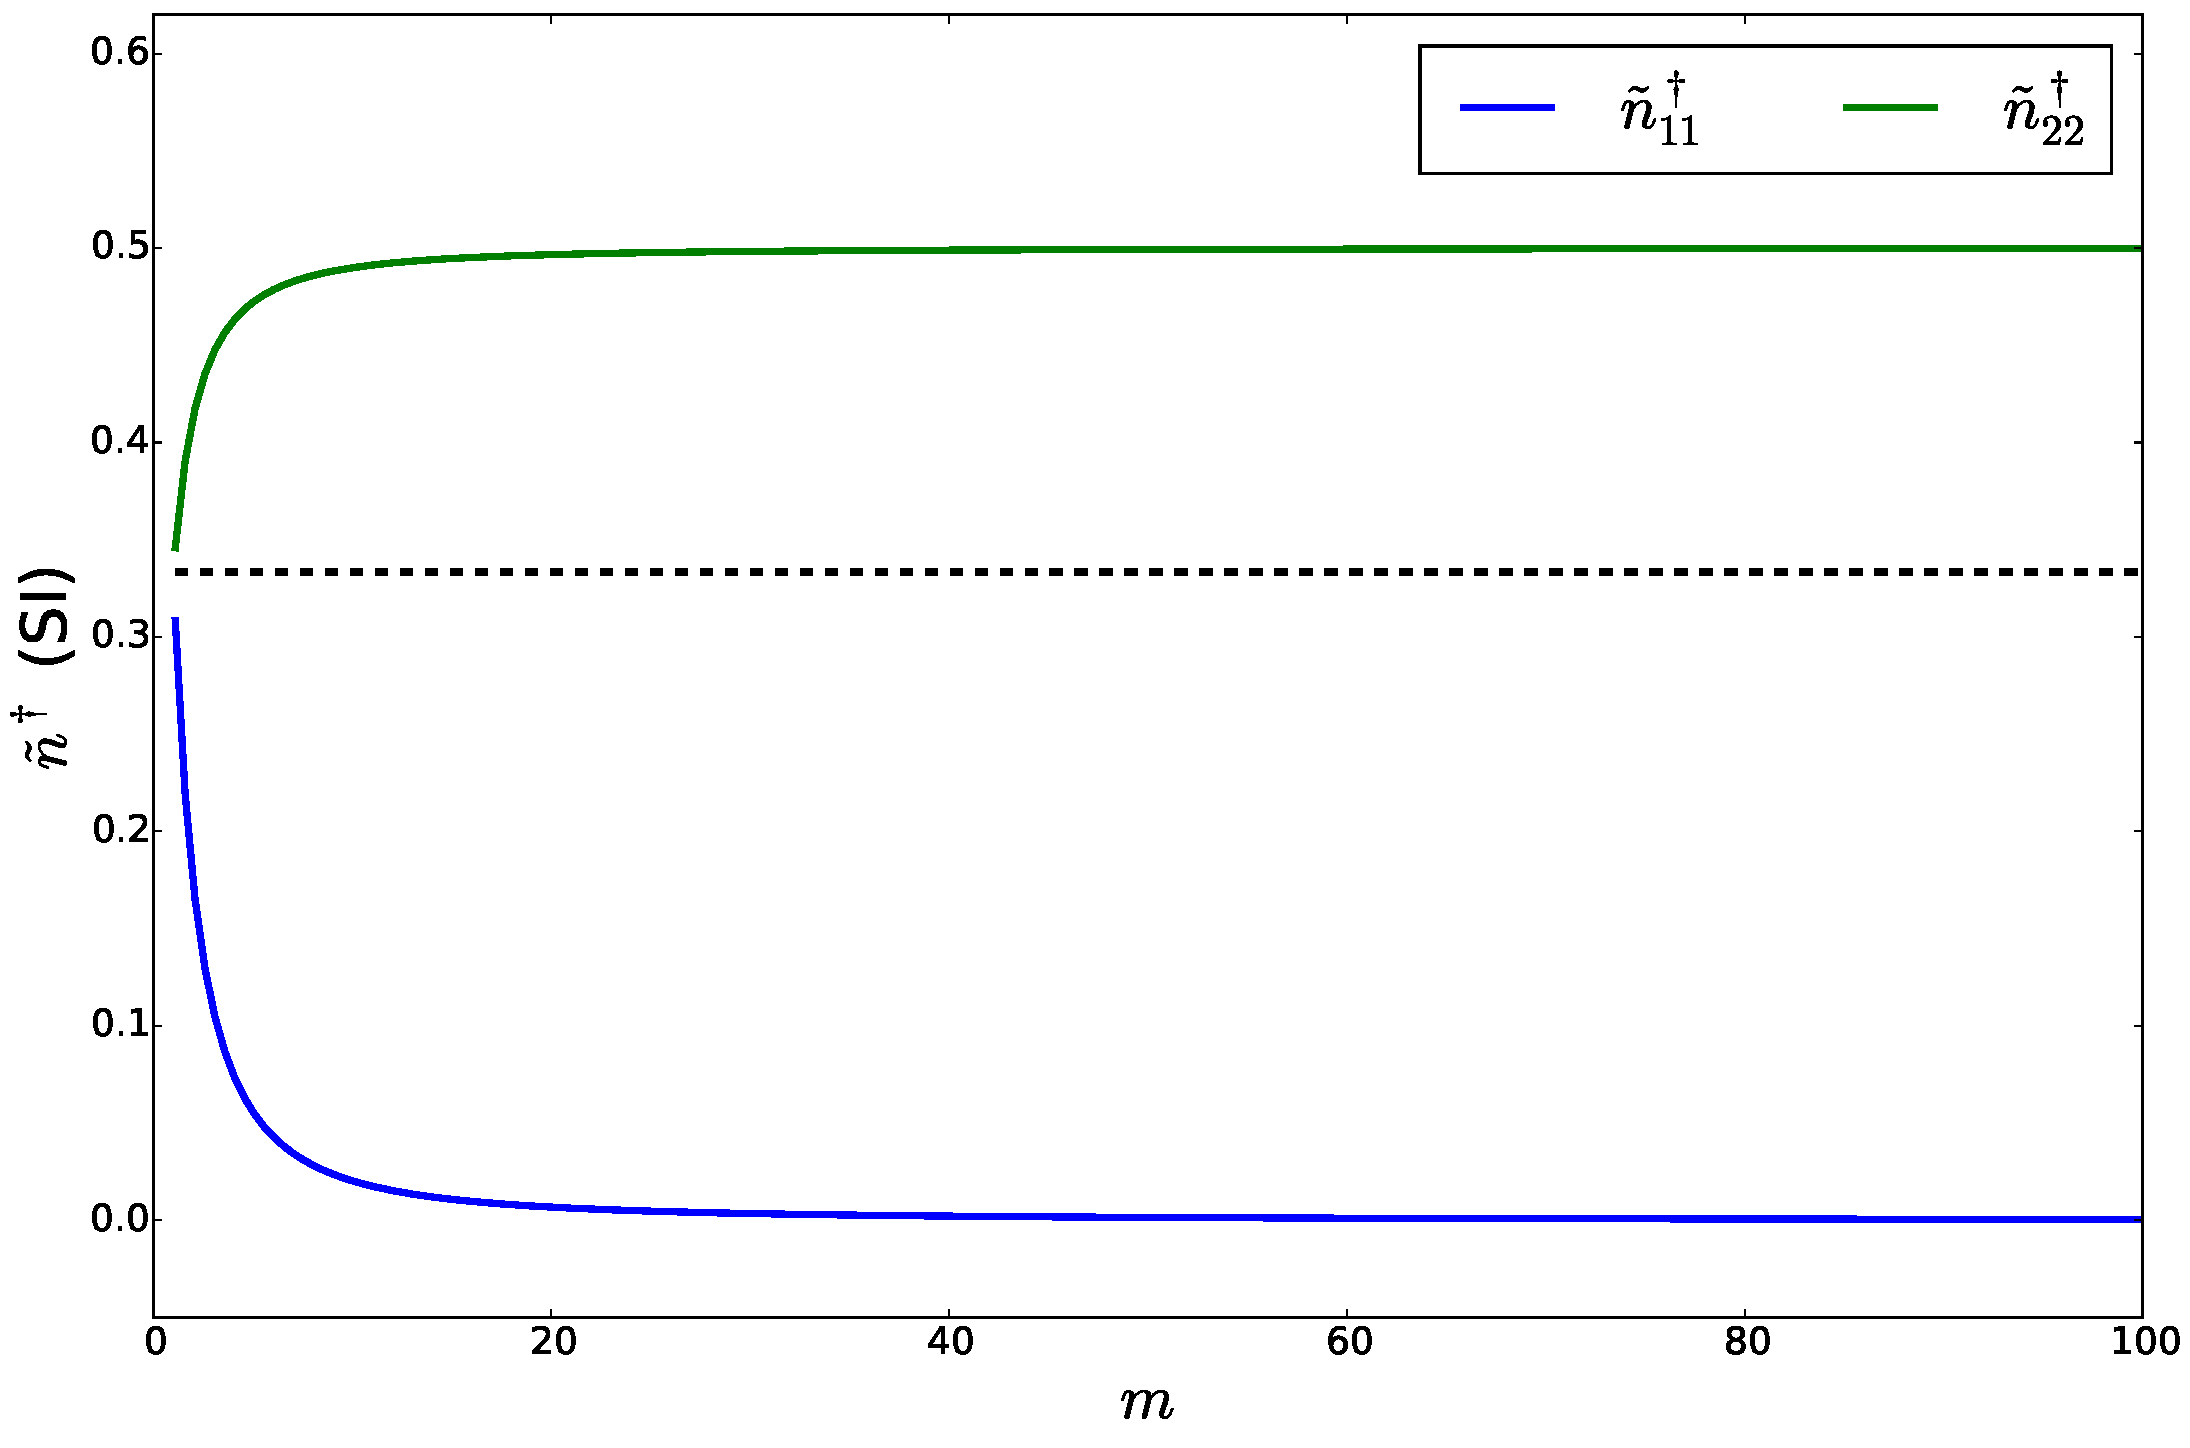
\includegraphics[width=15cm,height=10cm]{figures/test_n_prolate}
	\caption[Teste dos fatores de desmagnetização para um elipsoide prolato.]{Teste dos fatores de desmagnetização:
		$\tilde{n}^{\dagger}_{11}$ e $\tilde{n}^{\dagger}_{22}$
		para um elipsoide prolato originalmente com semi-eixos 110 e 100 metros, com um fator $m (a/b)$ crescente,
		aumentando a valor do semi-eixo maior e mantendo o semi-eixo menor constante.}
	\label{fig:n_prolato}
\end{figure}

Já na figura \ref{fig:n_oblato}realizamos a mesma relação entre os semi-eixos $a$ e $b$ do caso prolato, onde aumenta-se o valor de $a$. Lembremos que no caso do elipsoide oblato $a$ é o semi-eixo menor e $b$ o semi-eixo maior. No começo, quando os semi-eixos estão afastados, os elementos estão afastados para $b$ muito maior que $a$ e tendem à $1/3$ conforme se aproximam.
\newpage

\begin{figure}[hbt!]
	\centering 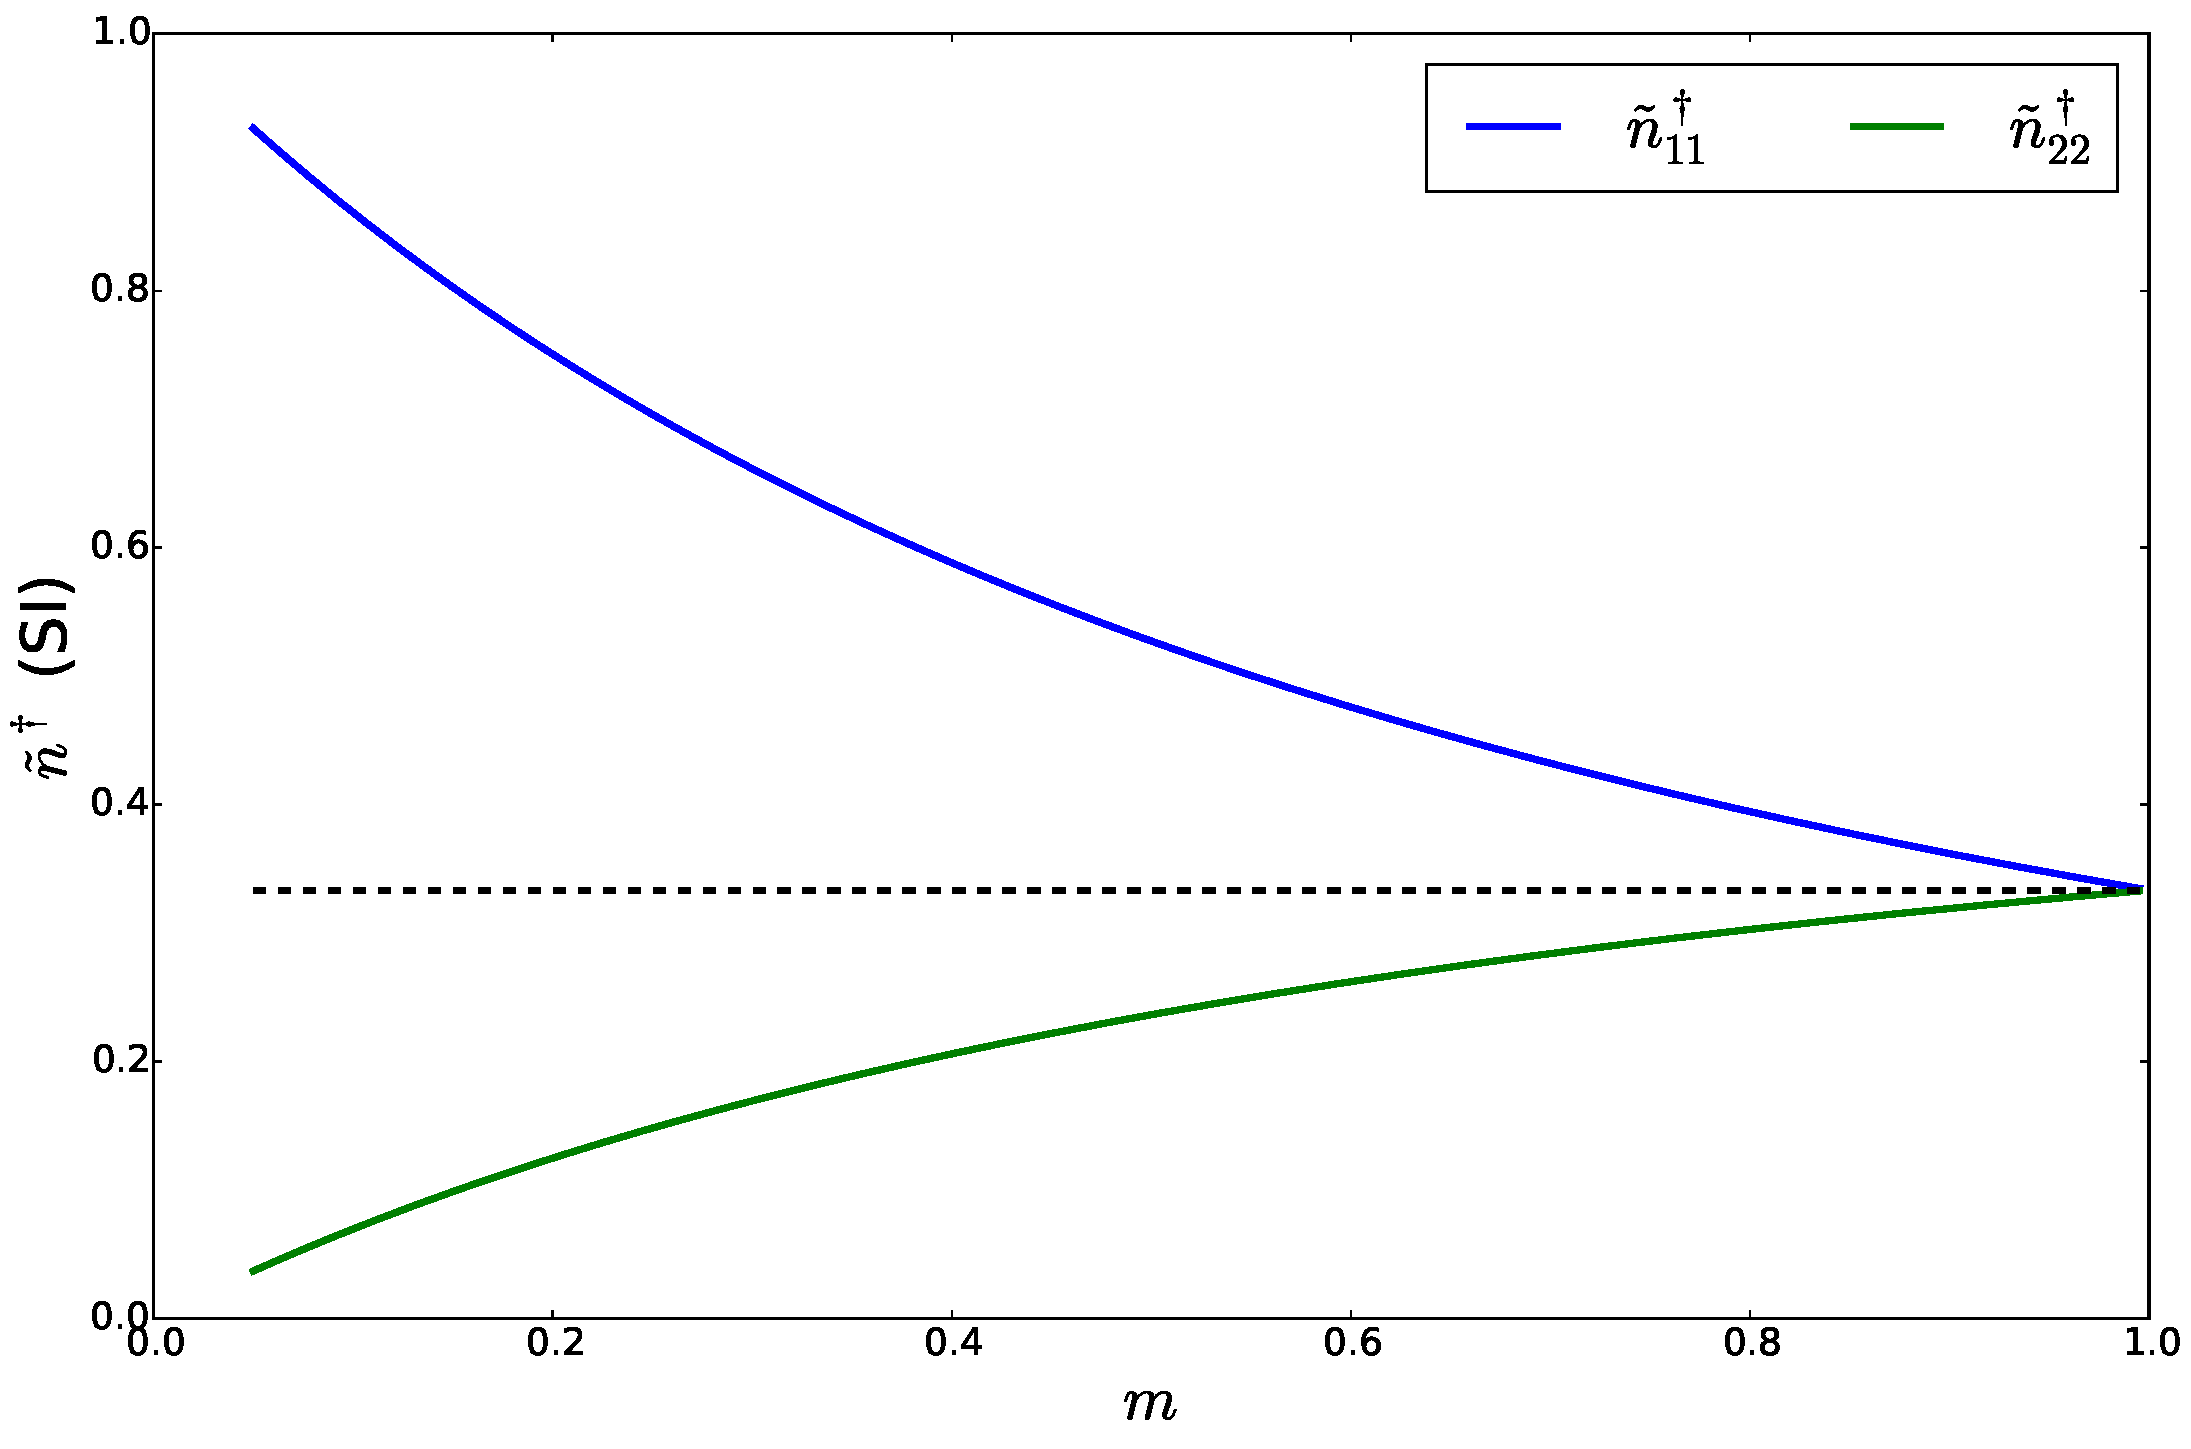
\includegraphics[width=15cm,height=10cm]{figures/test_n_oblate}
	\caption[Teste dos fatores de desmagnetização para um elipsoide oblato.]{Teste dos fatores de desmagnetização:
		$\tilde{n}^{\dagger}_{11}$ e $\tilde{n}^{\dagger}_{22}$
		para um elipsoide oblato originalmente com semi-eixos 1000 e 50 metros, com um fator $u (a/b)$ crescente,
		mantendo o semi-eixo maior constante (neste caso o $b$), e tornando o semi-eixo menor maior, até o ponto de
		quase se igualarem.}
	\label{fig:n_oblato}
\end{figure}

Através destes gráficos é possível observar como os fatores de desmagnetização possuem valor menor, quanto maior o semi-eixo do elipsoide. De fato há uma relação: $\tilde{n}^{\dagger}_{11}$ está relacionado com o semi-eixo maior, $\tilde{n}^{\dagger}_{22}$ com o semi-eixo intermediário e $\tilde{n}^{\dagger}_{33}$ com o semi-eixo menor. Fisicamente, isto significa que há a tendência, do elipsoide se desmagnetizar com maior intensidade na direção dos seus semi-eixos menores.

\section{Comparações entre os modelos elipsoidais}

Testamos a implementação computacional comparando com resultados conhecidos. Na Figura \ref{fig:triaxial_sphere} comparamos um elipsoide triaxial com seus três semi-eixos muito próximos um do outro (simulando uma esfera), conforme Tabela 4.5, e comparamos com a implementação da esfera do software \textit{Fatiando a Terra}.
\newpage

\begin{table}[h!]
	\begin{center}
		\begin{tabular}{lc}
			
			&  \\
			& \\
			& \\
			& \\
			& \\
			& \\
			& \\
			& \\
			& \\
			& \\
			& \\
			& \\
			& \\
		\end{tabular}
	\end{center}
\end{table}

\begin{table}[h!]
	\begin{center}
		\begin{tabular}{|l|c|c|}
			\hline
			\textbf{Parâmetro}  & \textbf{Valor}  & \textbf{Unidade}\\
			\hline 
			a, b, c   & 500.0001, 500.0, 499.9999   & m\\
			\hline
			Azimute   & $0$ & º\\
			\hline
			$\delta$    & $0$ & º\\
			\hline
			$\gamma$   & $0$  & º\\
			\hline
			xc   & 0  & m\\
			\hline          
			yc   & 0  & m\\
			\hline                
			zc   & 1000  & m\\
			\hline
			$J_{NRM}$*  & 100, $25^o$, $40^o$  & A/m\\
			\hline
			F*    & 1, $50^o$, $20^o$ & nT\\
			\hline
			k1, k2, k3   & 0.1, 0.1, 0.1 & SI \\
			\hline
			Orientações k**   & $0$, $90$, $90$  & º\\
			\hline
		\end{tabular}
		\caption{Parâmetros do elipsoide triaxial modelado para comparação com a esfera. *Valores de intensidade, inclinação e declinação respectivamente. **Ângulo de azimute, $\delta$ e $\gamma$, respectivamente, para as orientações da susceptibilidade.}
	\end{center}
	\label{tab:triaxial_sphere}
\end{table}

\begin{table}[h!]
	\begin{center}
		\begin{tabular}{lc}
			
			&  \\
			& \\
			& \\
			& \\
			& \\
			& \\
			& \\
			& \\
			& \\
			& \\
			& \\
			& \\
				
		\end{tabular}
	\end{center}
\end{table}

\begin{figure}[hbt!]
	\centering 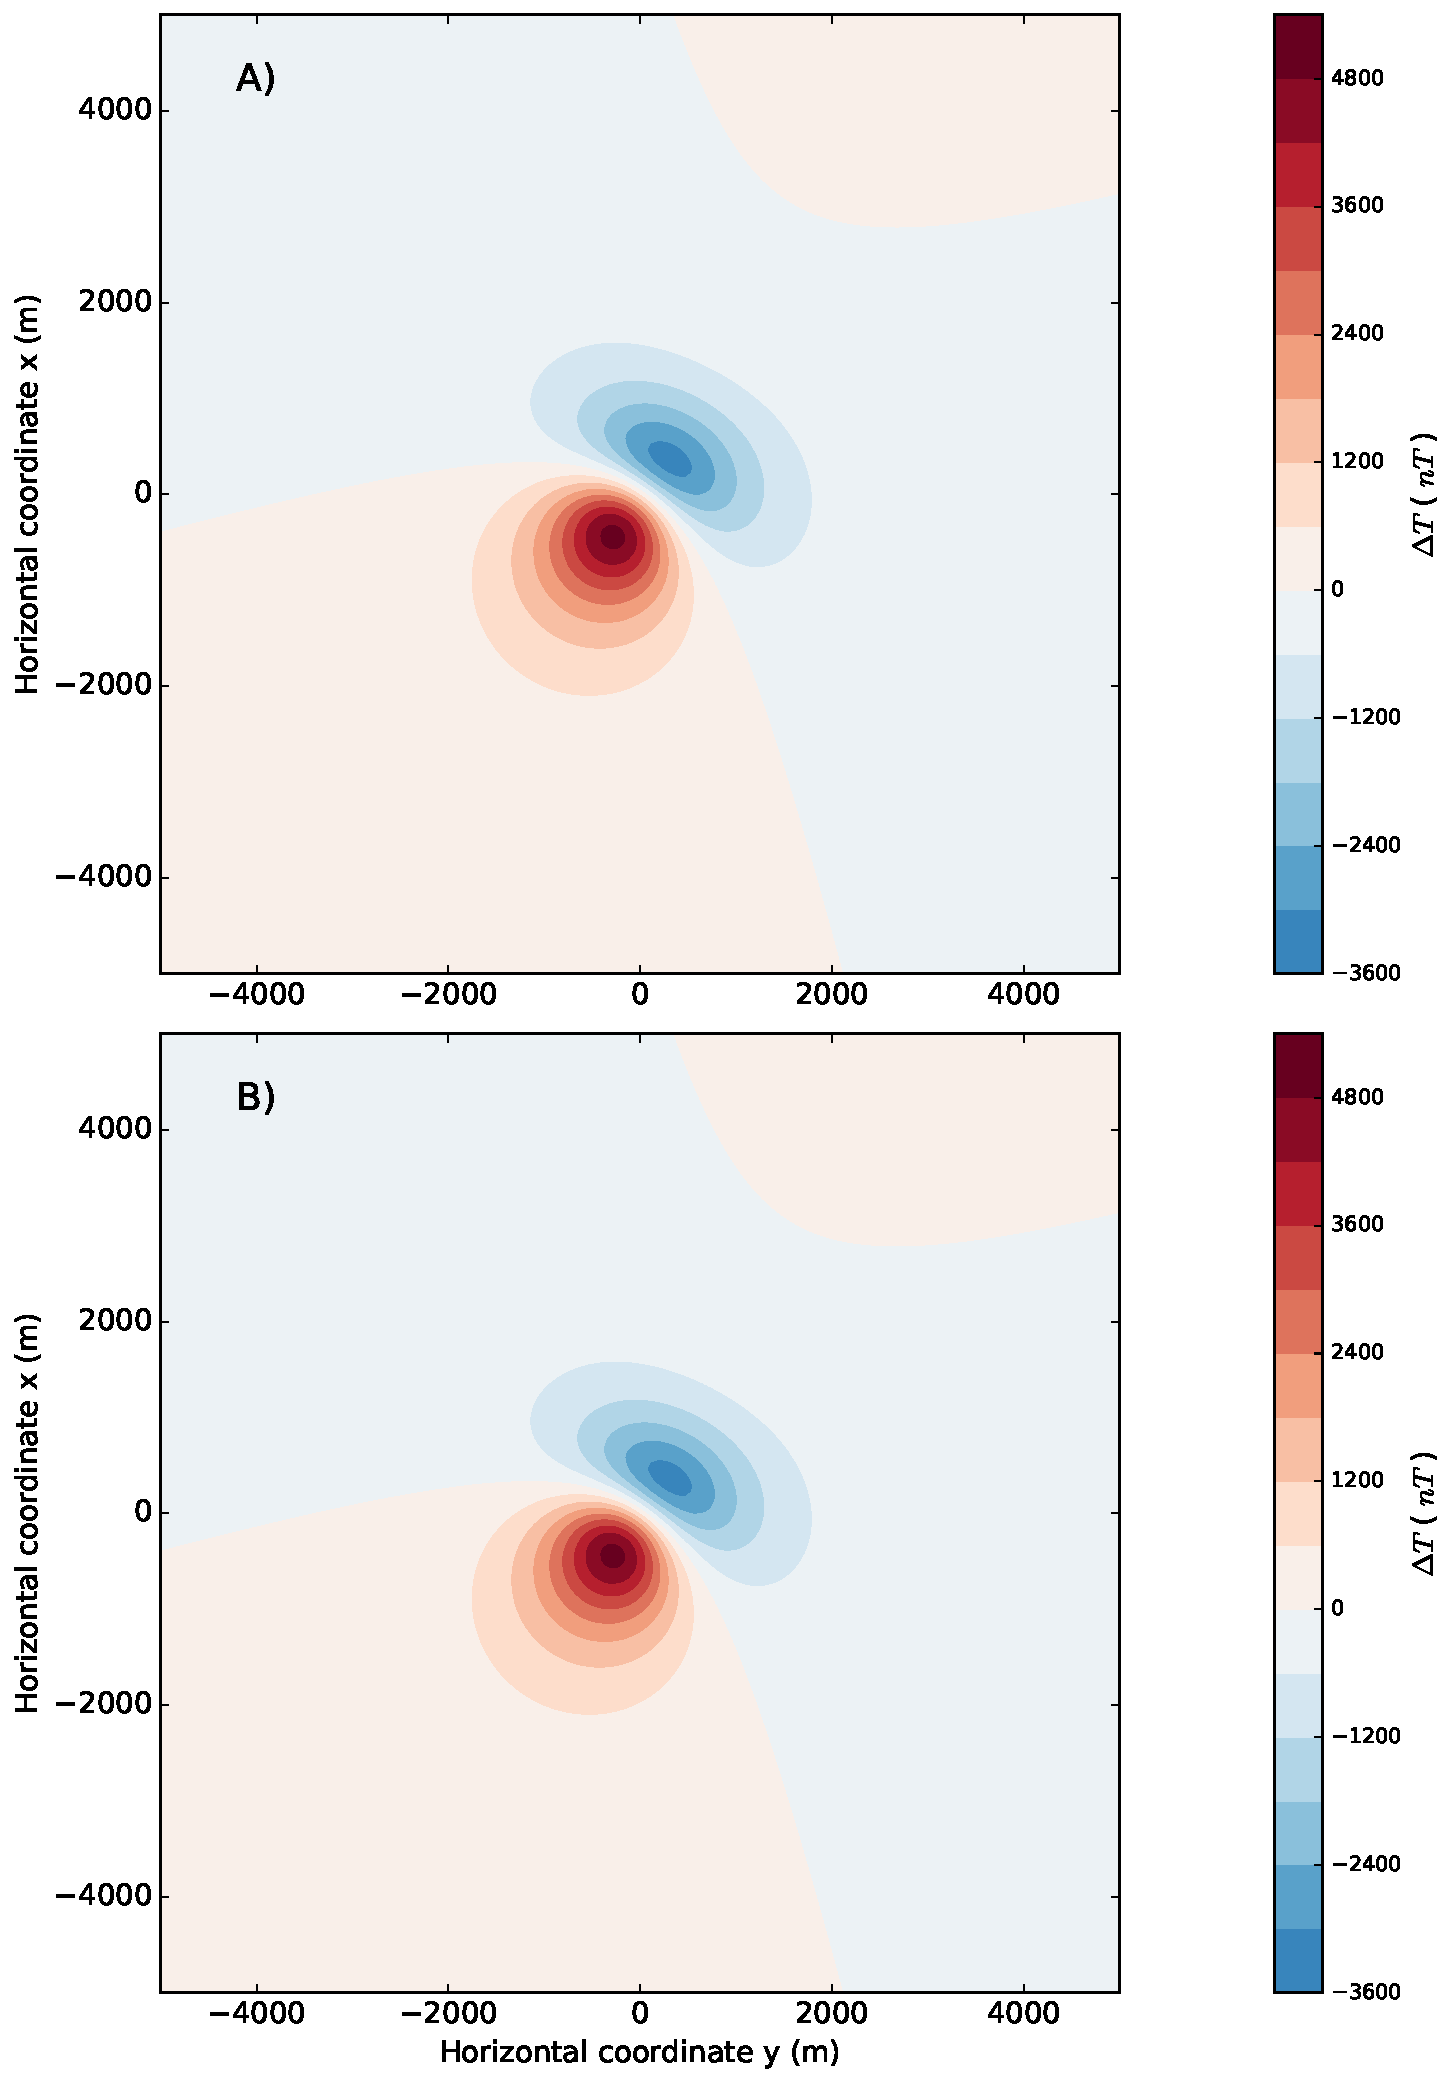
\includegraphics[width=14.5 cm,height=22 cm]{figures/ellipsoid_triaxial_sphere}
	\caption[Comparação da anomalia de campo total aproximada entre um elipsoide triaxial com três semi-eixos muito próximos, simulando uma esfera, 
	e uma esfera.]{Comparação da anomalia de campo total aproximada entre um elipsoide triaxial com três semi-eixos muito próximos, simulando uma esfera, e uma esfera implementada pelo software \textit{Fatiando a Terra}.}
	\label{fig:triaxial_sphere}
\end{figure}

Os resultados da comparação foram muito próximos. Confirmado a implementação do elipsoide triaxial, o usamos para comparar com a implementação do elipsoide prolato de parâmetros conforme tabelas 4.6 e 4.7. O resultado está na Figura \ref{fig:triaxial_prolate}.

\begin{table}[h!]
	\begin{center}
		\begin{tabular}{|l|c|c|}
			\hline
			\textbf{Parâmetro}  & \textbf{Valor}  & \textbf{Unidade} \\
			\hline 
			a, b, c  & 500, 100, 99.99 & m\\
			\hline
			Azimute   & $90$ & º\\
			\hline
			$\delta$    & $45$ & º\\
			\hline
			$\gamma$   & $0$  & º\\
			\hline
			xc   & 0 & m \\
			\hline          
			yc   & 0  & m\\
			\hline                
			zc   & 1000  & m\\
			\hline
			$J_{NRM}$*  & 100, $90^o$, $0^o$  & nT\\
			\hline
			F*    & 60000, $50^o$, $20^o$ & A/m\\
			\hline
			k1, k2, k3   & 0.2, 0.1, 0.05  & SI\\
			\hline
			Orientações k**   & $0$, $90$, $90$  & º\\
			\hline
		\end{tabular}
		\caption{Parâmetros do elipsoide triaxial modelado para comparação com o elipsoide prolato. *Valores de intensidade, inclinação e declinação respectivamente. **Ângulo de azimute, $\delta$ e $\gamma$, respectivamente, para as orientações da susceptibilidade.}
	\end{center}
	\label{tab:triaxial_prolate1}
\end{table}

\vspace{2cm}

\begin{table}[h!]
	\begin{center}
		\begin{tabular}{|l|c|c|}
			\hline
			\textbf{Parâmetro}  & \textbf{Valor}  & \textbf{Unidade}\\
			\hline 
			a, b  & 500, 100 & m\\
			\hline
			Azimute   & $90$ & m\\
			\hline
			$\delta$    & $45$ & º\\
			\hline
			$\gamma$   & $0$  & º\\
			\hline
			xc   & 0  & m\\
			\hline          
			yc   & 0  & m\\
			\hline                
			zc   & 1000  & m\\
			\hline
			$J_{NRM}$*  & 100, $90^o$, $0^o$  & A/m\\
			\hline
			F*    & 60000, $50^o$, $20^o$ & nT\\
			\hline
			k1, k2, k3   & 0.2, 0.1, 0.05  & SI\\
			\hline
			Orientações k**   & $0$, $90$, $90$  & º\\
			\hline
		\end{tabular}
		\caption{Parâmetros do elipsoide prolato modelado para comparação com elipsoide triaxial. *Valores de intensidade, inclinação e declinação respectivamente. **Ângulo de azimute, $\delta$ e $\gamma$, respectivamente, para as orientações da susceptibilidade.}
	\end{center}
	\label{tab:triaxial_prolate2}
\end{table}

\begin{figure}[hbt!]
	\centering \includegraphics[width=14.5 cm,height=22 cm]{figures/ellipsoid_triaxial_prolate}
	\caption[Comparação da anomalia de campo total aproximada entre um elipsoide triaxial com um dos semi-eixos mais alongado que o 
	restante e um elipsoide prolato.]{Comparação da anomalia de campo total aproximada entre um elipsoide triaxial com um dos semi-eixos mais alongado que o restante e um elipsoide prolato.}
	\label{fig:triaxial_prolate}
\end{figure}

Também usamos a implementação do elipsoide triaxial, para comparar com a implementação do elipsoide oblato de parâmetros conforme tabelas 4.8 e 4.9. O resultado está na Figura \ref{fig:triaxial_oblate}.

\begin{table}[h!]
	\begin{center}
		\begin{tabular}{|l|c|c|}
			\hline
			\textbf{Parâmetro}  & \textbf{Valor} & \textbf{Unidade} \\
			\hline 
			a, b, c   & 500, 499.99, 499.98 & m\\
			\hline
			Azimute   & $0$ & m\\
			\hline
			$\delta$    & $0$ & º\\
			\hline
			$\gamma$   & $90$  & º\\
			\hline
			xc   & 0  & m\\
			\hline          
			yc   & 0  & m\\
			\hline                
			zc   & 1000 & m \\
			\hline
			$J_{NRM}$*  & 100, $90^o$, $0^o$ & A/m \\
			\hline
			F*    & 60000, $50^o$, $20^o$ & nT \\
			\hline
			k1, k2, k3   & 0.1, 0.1, 0.1 & SI \\
			\hline
			Orientações k**   & $0$, $90$, $90$ & º \\
			\hline
		\end{tabular}
		\caption{Parâmetros do elipsoide triaxial modelado para comparação com o elipsoide oblato. *Valores de intensidade, inclinação e declinação respectivamente. **Ângulo de azimute, $\delta$ e $\gamma$, respectivamente, para as orientações da susceptibilidade.}
	\end{center}
	\label{tab:triaxial_oblate1}
\end{table}

\vspace{2cm}

\begin{table}[h!]
	\begin{center}
		\begin{tabular}{|l|c|c|}
			\hline
			\textbf{Parâmetro}  & \textbf{Valor} & \textbf{Unidade} \\
			\hline 
			a, b   & 499.99, 500 & m\\
			\hline
			Azimute   & $0$ & º\\
			\hline
			$\delta$    & $0$ & º\\
			\hline
			$\gamma$   & $0$  & º\\
			\hline
			xc   & 0  & m\\
			\hline          
			yc   & 0  & m\\
			\hline                
			zc   & 1000  & m\\
			\hline
			$J_{NRM}$*  & 100, $90^o$, $0^o$  & A/m\\
			\hline
			F*    & 60000, $50^o$, $20^o$ & nT \\
			\hline
			k1, k2, k3   & 0.1, 0.1, 0.1 & SI \\
			\hline
			Orientações k**   & $0$, $90$, $90$ & º \\
			\hline
		\end{tabular}
		\caption{Parâmetros do elipsoide oblato modelado para compração com o elipsoide triaxial. *Valores de intensidade, inclinação e declinação respectivamente. **Ângulo de azimute, $\delta$ e $\gamma$, respectivamente, para as orientações da susceptibilidade.}
	\end{center}
	\label{tab:triaxial_oblate2}
\end{table}

\begin{figure}[hbt!]
	\centering \includegraphics[width=14.5 cm,height=22 cm]{figures/ellipsoid_triaxial_oblate}
	\caption[Comparação da anomalia de campo total aproximada entre um elipsoide triaxial com três semi-eixos muito próximos 
	e um elipsoide oblato.]{Comparação da anomalia de campo total aproximada entre um elipsoide triaxial com três semi-eixos muito próximos e um elipsoide oblato também com seus dois semi-eixos muito próximos.}
	\label{fig:triaxial_oblate}
\end{figure}

\section{Susceptibilidade}

Em corpos de alta susceptibilidade, a desmagnetização é um fator muito importante, pois isso pode acarretar em erros de interpretação das anomalias em dados magnéticos. Na Figura \ref{fig:test_k_triaxial}, mostramos com um aumento gradual da susceptibilidade (neste caso isotrópica), a diferença na inclinação e declinação que o vetor de magnetização resultante sofre. É conhecido na literatura que o valor de susceptibilidade de 0.1 SI é o ponto onde a desmagnetização não deve ser desconsiderada na modelagem, o que de fato observa-se neste gráfico.

\begin{figure}[hbt!]
	\centering 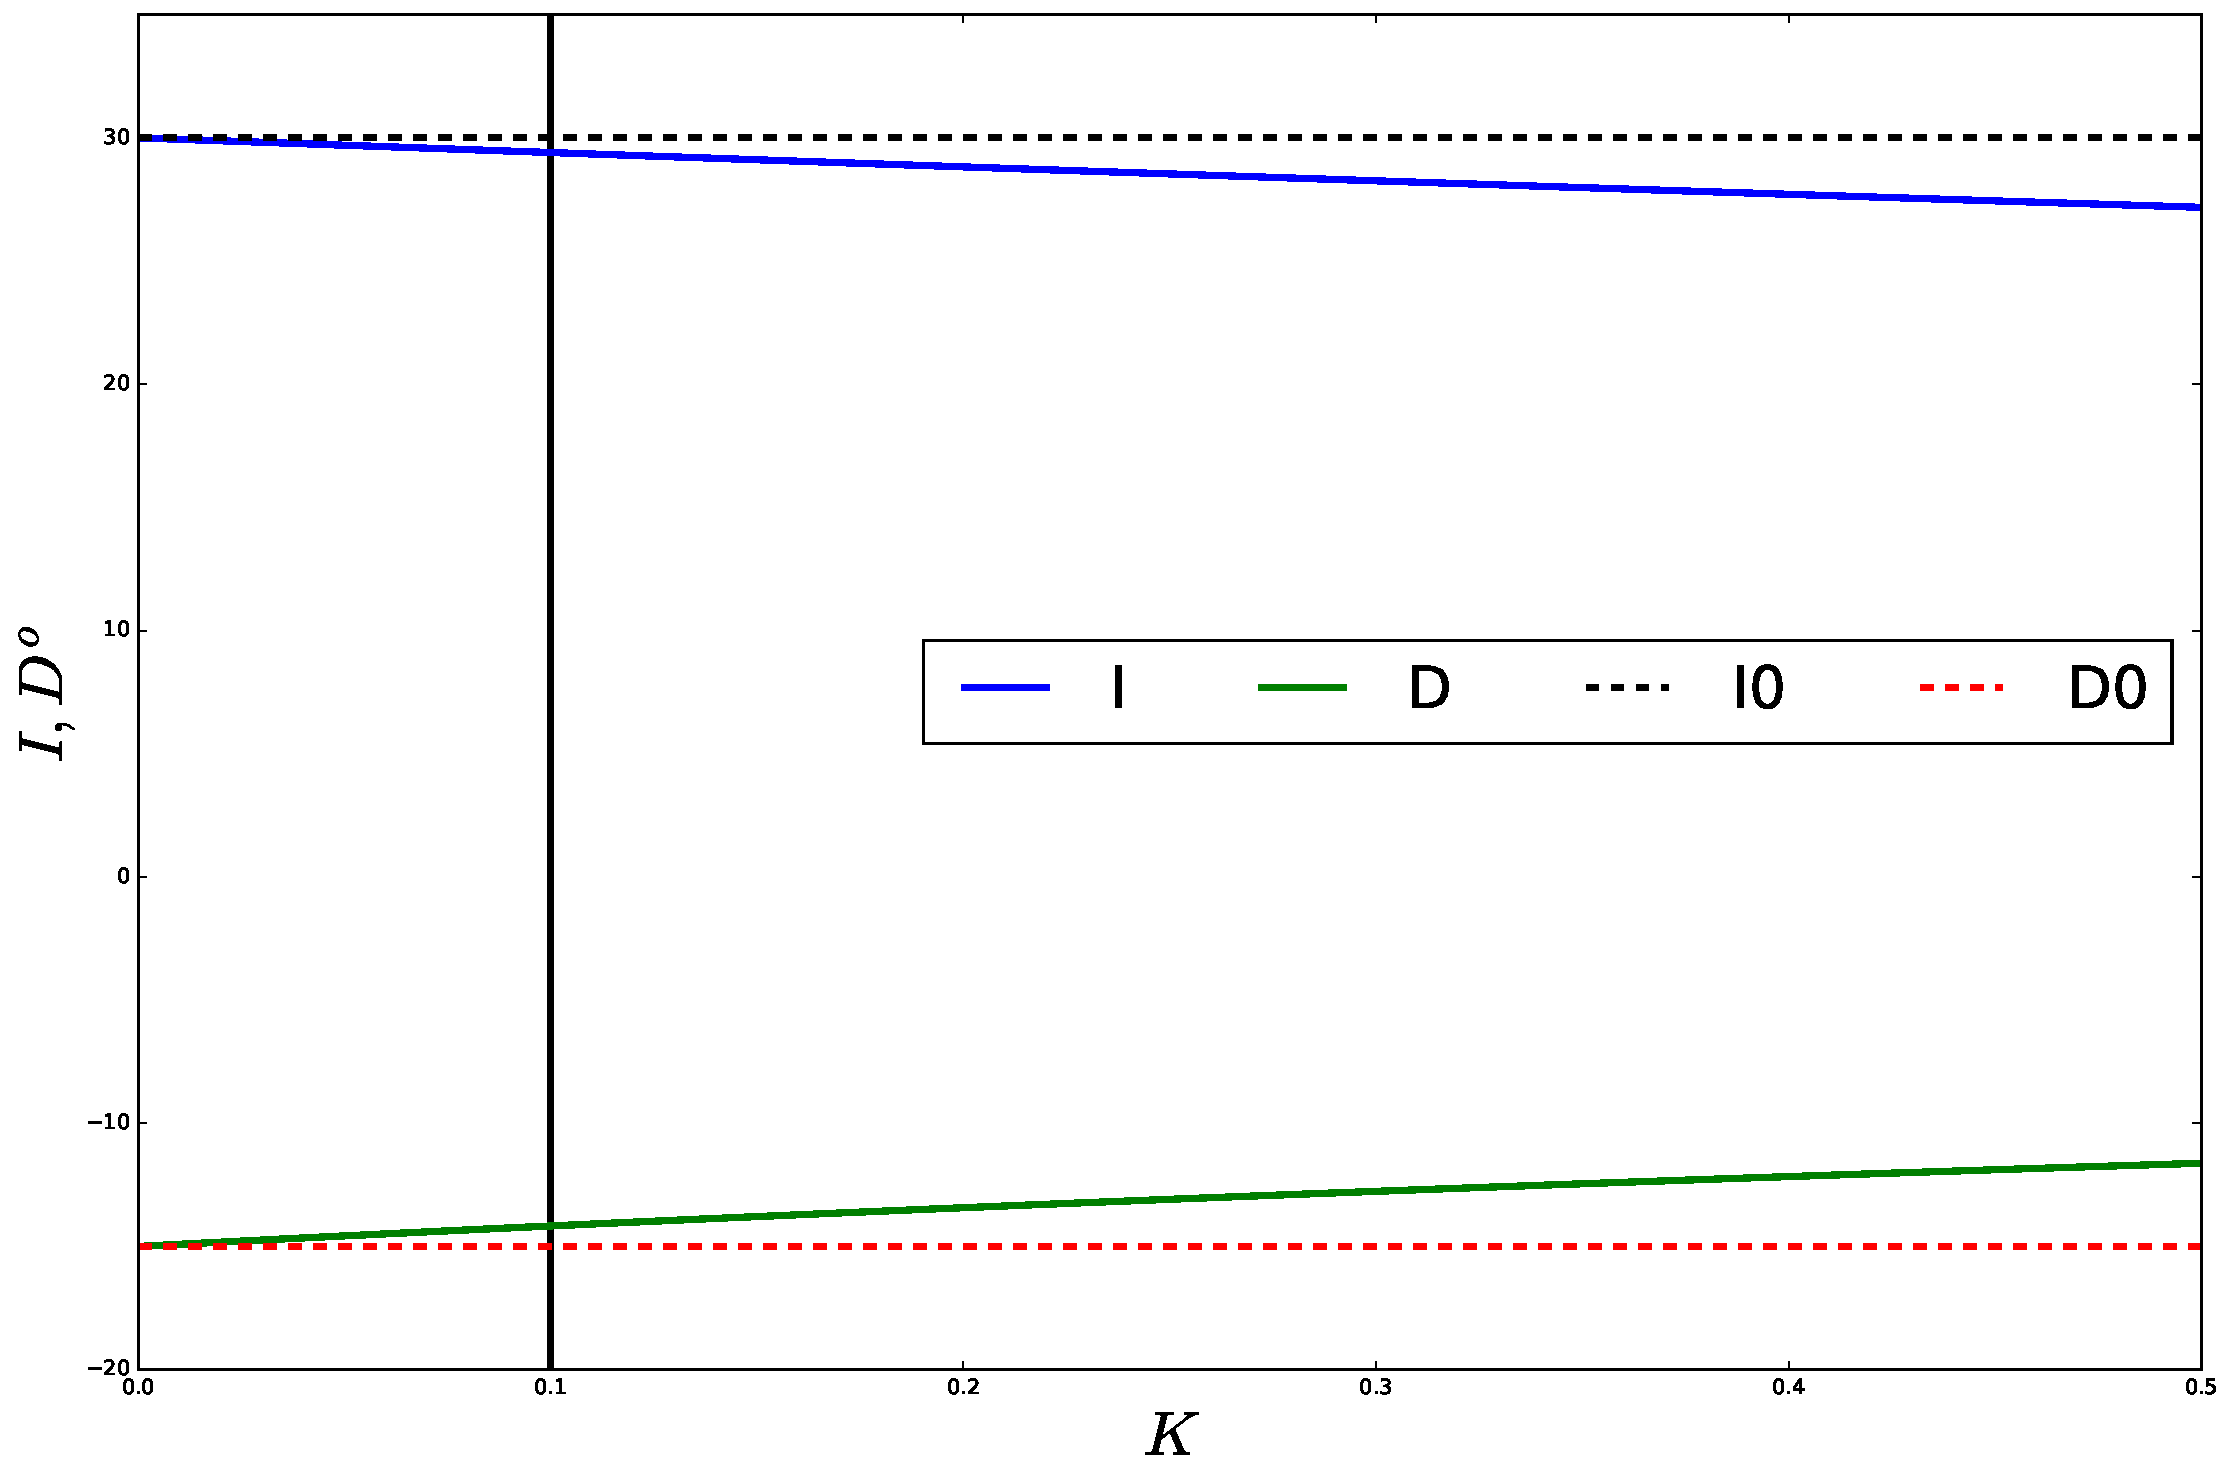
\includegraphics[width=15 cm,height=10 cm]{figures/test_k_triaxial}
	\caption[Teste do efeito da susceptibilidade na desmagnetização de um elipsoide imerso em um campo externo constante de inclinação 
	$30^{o}$ e declinação $-15^{o}$.]{Teste do efeito da susceptibilidade na desmagnetização de um elipsoide imerso em um campo externo constante de inclinação	$30^{o}$ e declinação $-15^{o}$, sem magnetização remanente, que recebe gradativamente, de forma isotrópica,
		uma susceptibilidade crescente. Em destaque uma linha demarcatória em $K=0.1$ SI, onde a literatura reconhece como um valor limite 
		para desconsiderar os efeitos da desmagnetização.}
	\label{fig:test_k_triaxial}
\end{figure}

\begin{table}[h!]
	\begin{center}
		\begin{tabular}{lc}
			
			&  \\
			& \\
			& \\
			& \\
			& \\
			
		\end{tabular}
	\end{center}
\end{table}

\section{Anisotropia de forma}

Conforme dito na seção 4.2 existe uma relação entre os elementos do tensor de depolarização e os semi-eixos. Na Figura \ref{fig:ellipsoid_shape_iso10} mostramos como o aumento do semi-eixo maior afeta o vetor de magnetização resultante. A princípio, os três semi-eixos estão muito próximos, simulando uma esfera. Quando postos sob um campo externo, o vetor de magnetização resultante se direciona para a direção deste campo. Porém a medida que aumenta-se o semi-eixo maior, ocorre a depolarização dos demais e o vetor de magnetização resultante tende a se alinhar na direção do semi-eixo maior (neste caso o elipsoide triaxial possui um azimute de 10$º$).

\vspace{2cm}

\begin{table}[h!]
	\begin{center}
		\begin{tabular}{|l|c|c|}
			\hline
			\textbf{Parâmetro}  & \textbf{Valor}  & \textbf{Unidade }\\
			\hline 
			a, b, c  & 50.1-1000, 50, 49.9 & m\\
			\hline
			Azimute   & $10$ & º \\
			\hline
			$\delta$    & $0$ & º\\
			\hline
			$\gamma$   & $0$  & º\\
			\hline
			xc   & 0  & m\\
			\hline          
			yc   & 0  & m\\
			\hline                
			zc   & 1000  & m\\
			\hline
			$J_{NRM}$*  & 100, $0^o$, $0^o$ & A/m \\
			\hline
			F*    & 60000, $90^o$, $20^o$ & nT\\
			\hline
			k1, k2, k3   & 50, 50, 50  & SI\\
			\hline
			Orientações k**   & $0$, $90$, $90$  & º\\
			\hline
		\end{tabular}
		\caption{Parâmetros do elipsoides triaxiais modelados com o semi-eixo $a$ crescente e azimute com grande diferença na direção com relação ao campo da Terra para verificar a anisotropia de forma. *Valores de intensidade, inclinação e declinação respectivamente. **Ângulo de azimute, $\delta$ e $\gamma$, respectivamente, para as orientações da susceptibilidade.}
	\end{center}
	\label{tab:ellipsoid_shape_iso10}
\end{table}

\begin{table}[h!]
	\begin{center}
		\begin{tabular}{lc}
			
			&  \\
			& \\
			& \\
			&  \\
			& \\
			& \\
			& \\
			& \\
			& \\
			& \\

			
		\end{tabular}
	\end{center}
\end{table}

\begin{figure}[hbt!]
	\centering 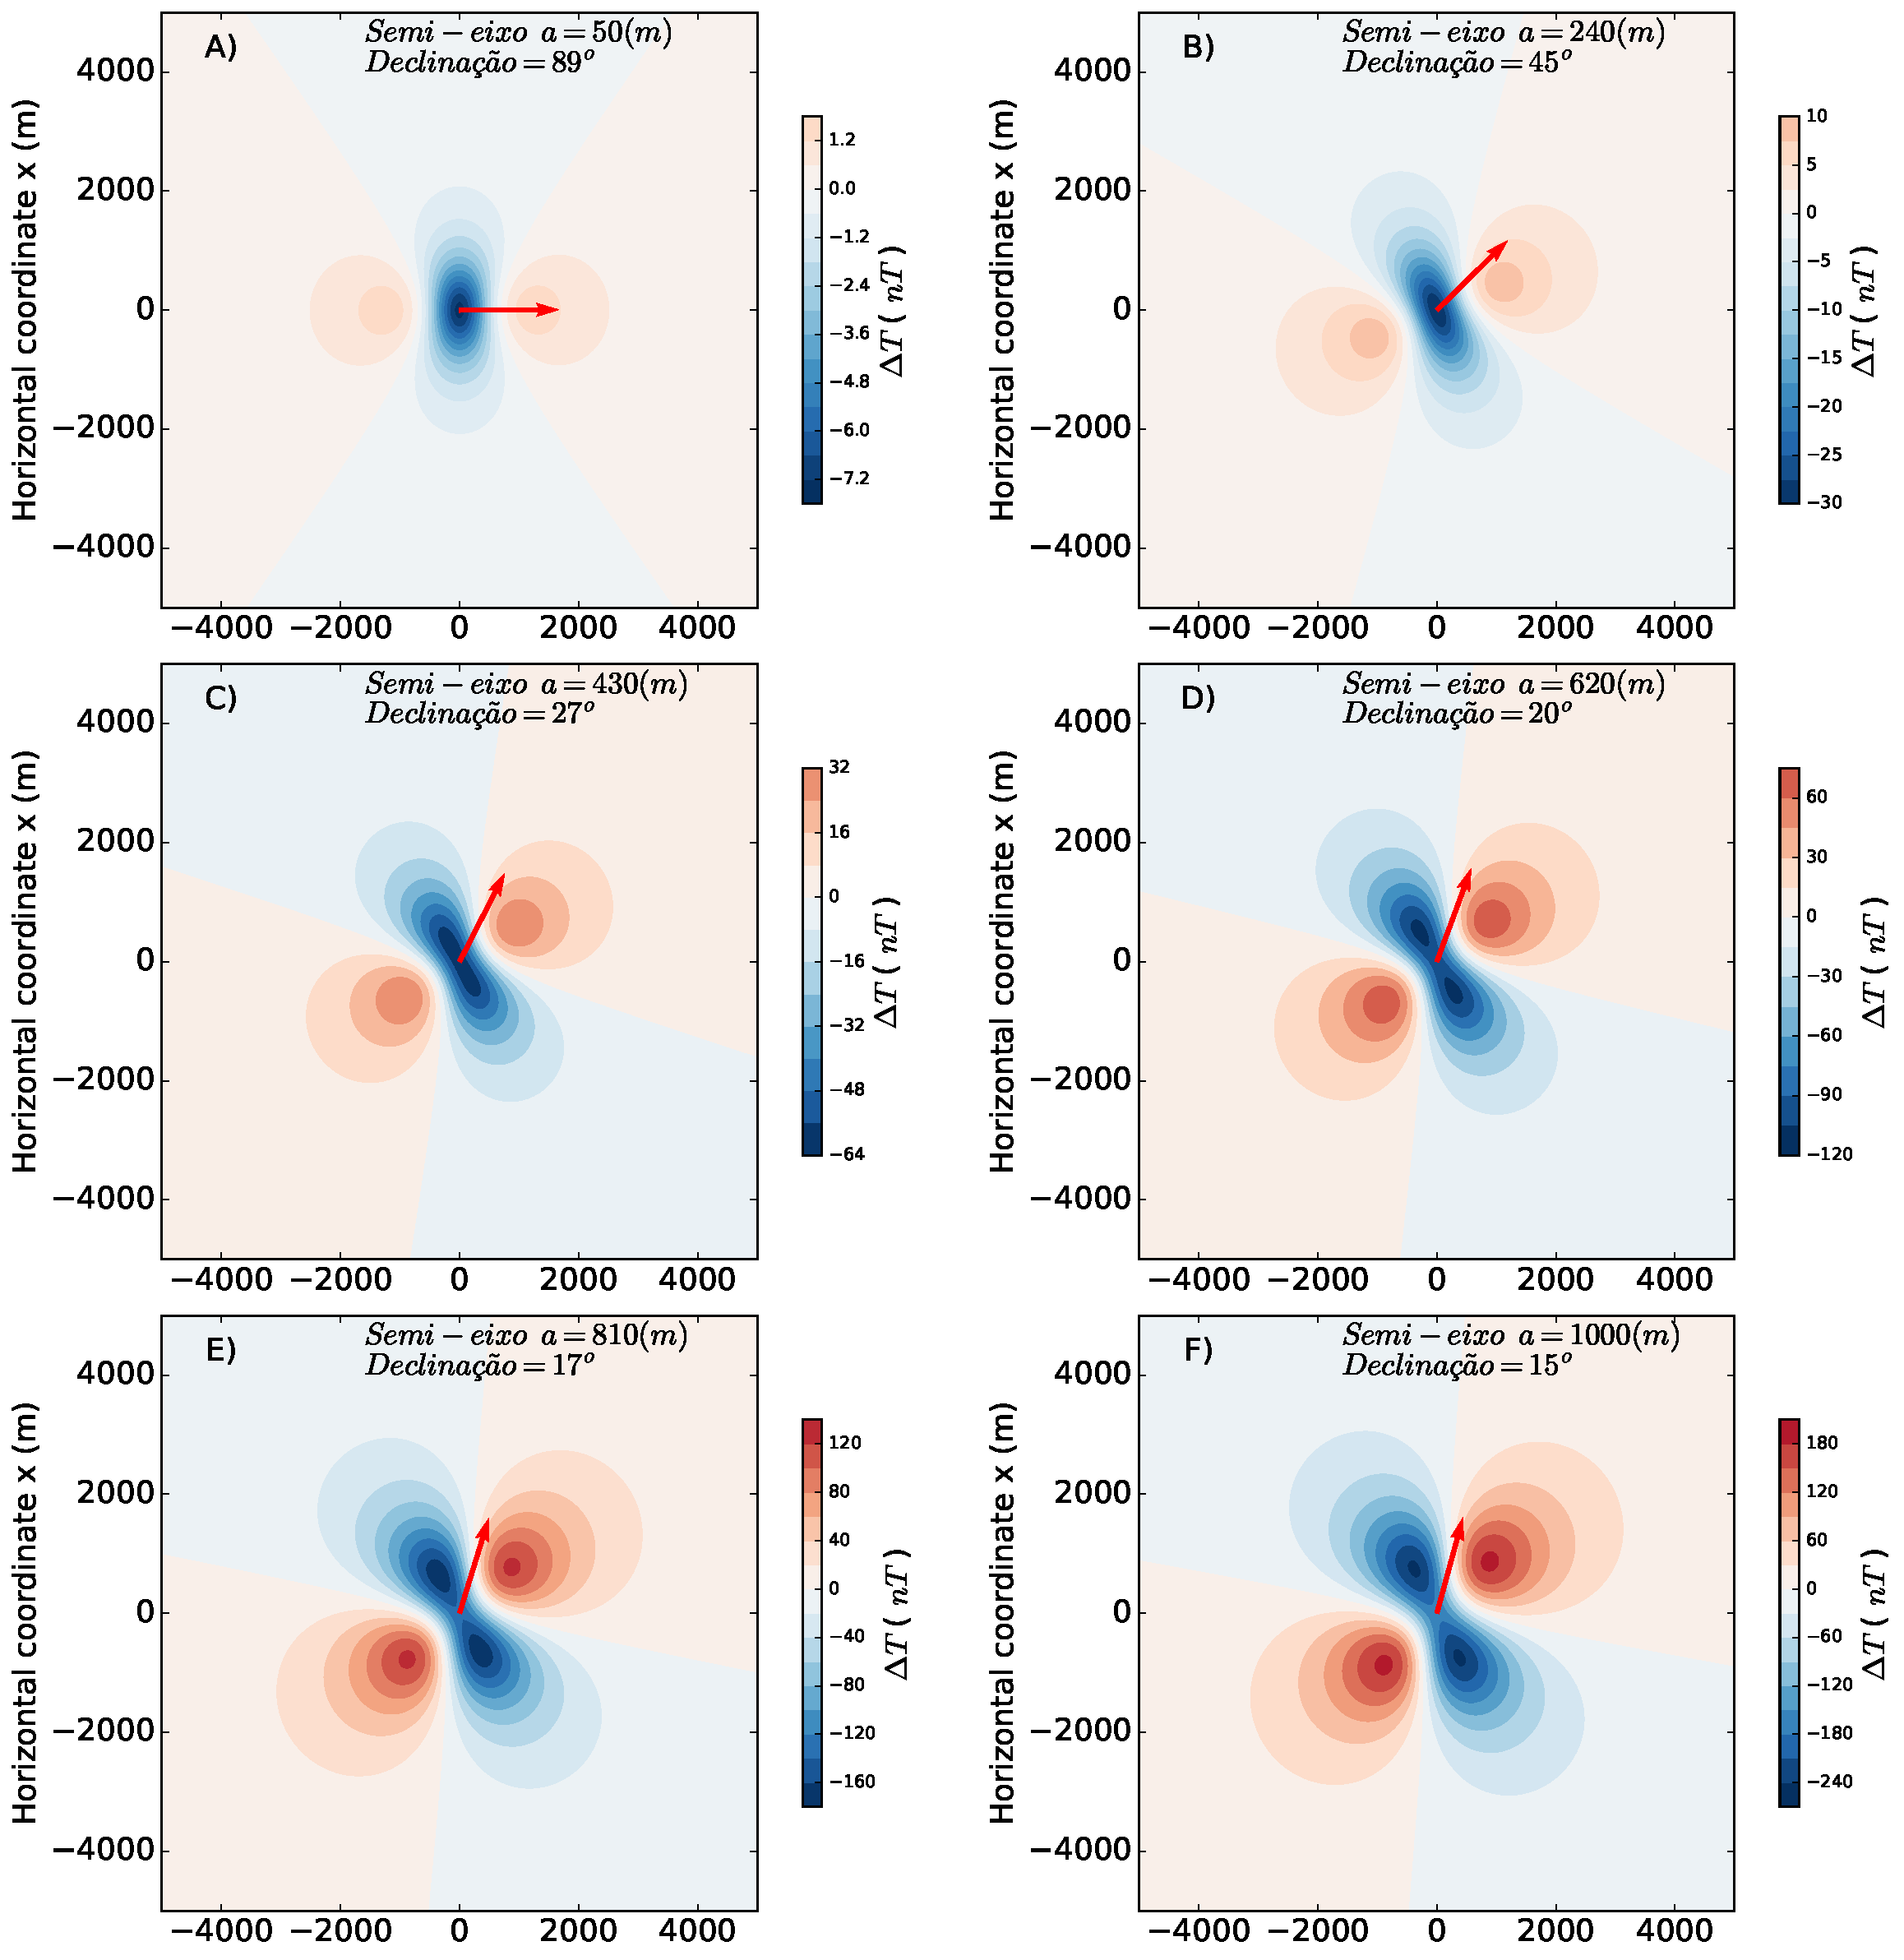
\includegraphics[width=16 cm,height=16 cm]{figures/ellipsoid_shape_iso}
	\caption[Simulação, da mudança do vetor de magnetização resultante, de um elipsoide triaxial com o aumento do semi-eixo maior.]{Simulação, da mudança do vetor de magnetização resultante, de um elipsoide triaxial com o aumento do semi-eixo maior. O elipsoide está imerso em um campo externo constante de declinação $90^o$, possui susceptibilidade isotrópica e constante e está direcionado com um azimute de $10^o$. Ao longo da sequência das figuras, seu semi-eixo maior aumenta de proporção em relação aos demais (variando entre 50 e 3000 m.). Nota-se a tendência do vetor de magnetização resultante (seta em vermelho) em se alinhar com o semi-eixo maior.}
	\label{fig:ellipsoid_shape_iso10}
\end{figure}

\begin{table}[h!]
	\begin{center}
		\begin{tabular}{lc}
			
			& \\
			& \\
			& \\
			& \\
			& \\
			
		\end{tabular}
	\end{center}
\end{table}

Para efeito de comparação realizamos o mesmo teste, porém com um azimute de 80$º$ para o elipsoide. A variação é bem menor, mas também se confirma a tendência do alinhamento do vetor de magnetização resultante para a direção do semi-eixo maior.

\vspace{2cm}

\begin{table}[h!]
	\begin{center}
		\begin{tabular}{|l|c|c|}
			\hline
			\textbf{Parâmetro}  & \textbf{Valor}  & \textbf{Unidade} \\
			\hline 
			a, b, c & 50.1-1000, 50, 49.9 & m\\
			\hline
			Azimute   & $80$ & º\\
			\hline
			$\delta$    & $0$ & º\\
			\hline
			$\gamma$   & $0$  & º\\
			\hline
			xc   & 0  & m\\
			\hline          
			yc   & 0  & m\\
			\hline                
			zc   & 1000  & m\\
			\hline
			$J_{NRM}$*  & 100, $0^o$, $0^o$  & A/m\\
			\hline
			F*    & 60000, $50^o$, $20^o$ & nT\\
			\hline
			k1, k2, k3   & 50, 50, 50  & SI\\
			\hline
			Orientações k**   & $0$, $90$, $90$  & º\\
			\hline
		\end{tabular}
		\caption{Parâmetros do elipsoides triaxiais modelados com o semi-eixo $a$ crescente e azimute com grande diferença na direção com relação ao campo da Terra para verificar a anisotropia de forma. *Valores de intensidade, inclinação e declinação respectivamente. **Ângulo de azimute, $\delta$ e $\gamma$, respectivamente, para as orientações da susceptibilidade.}
	\end{center}
	\label{tab:ellipsoid_shape_iso80}
\end{table}

\begin{figure}[hbt!]
	\centering 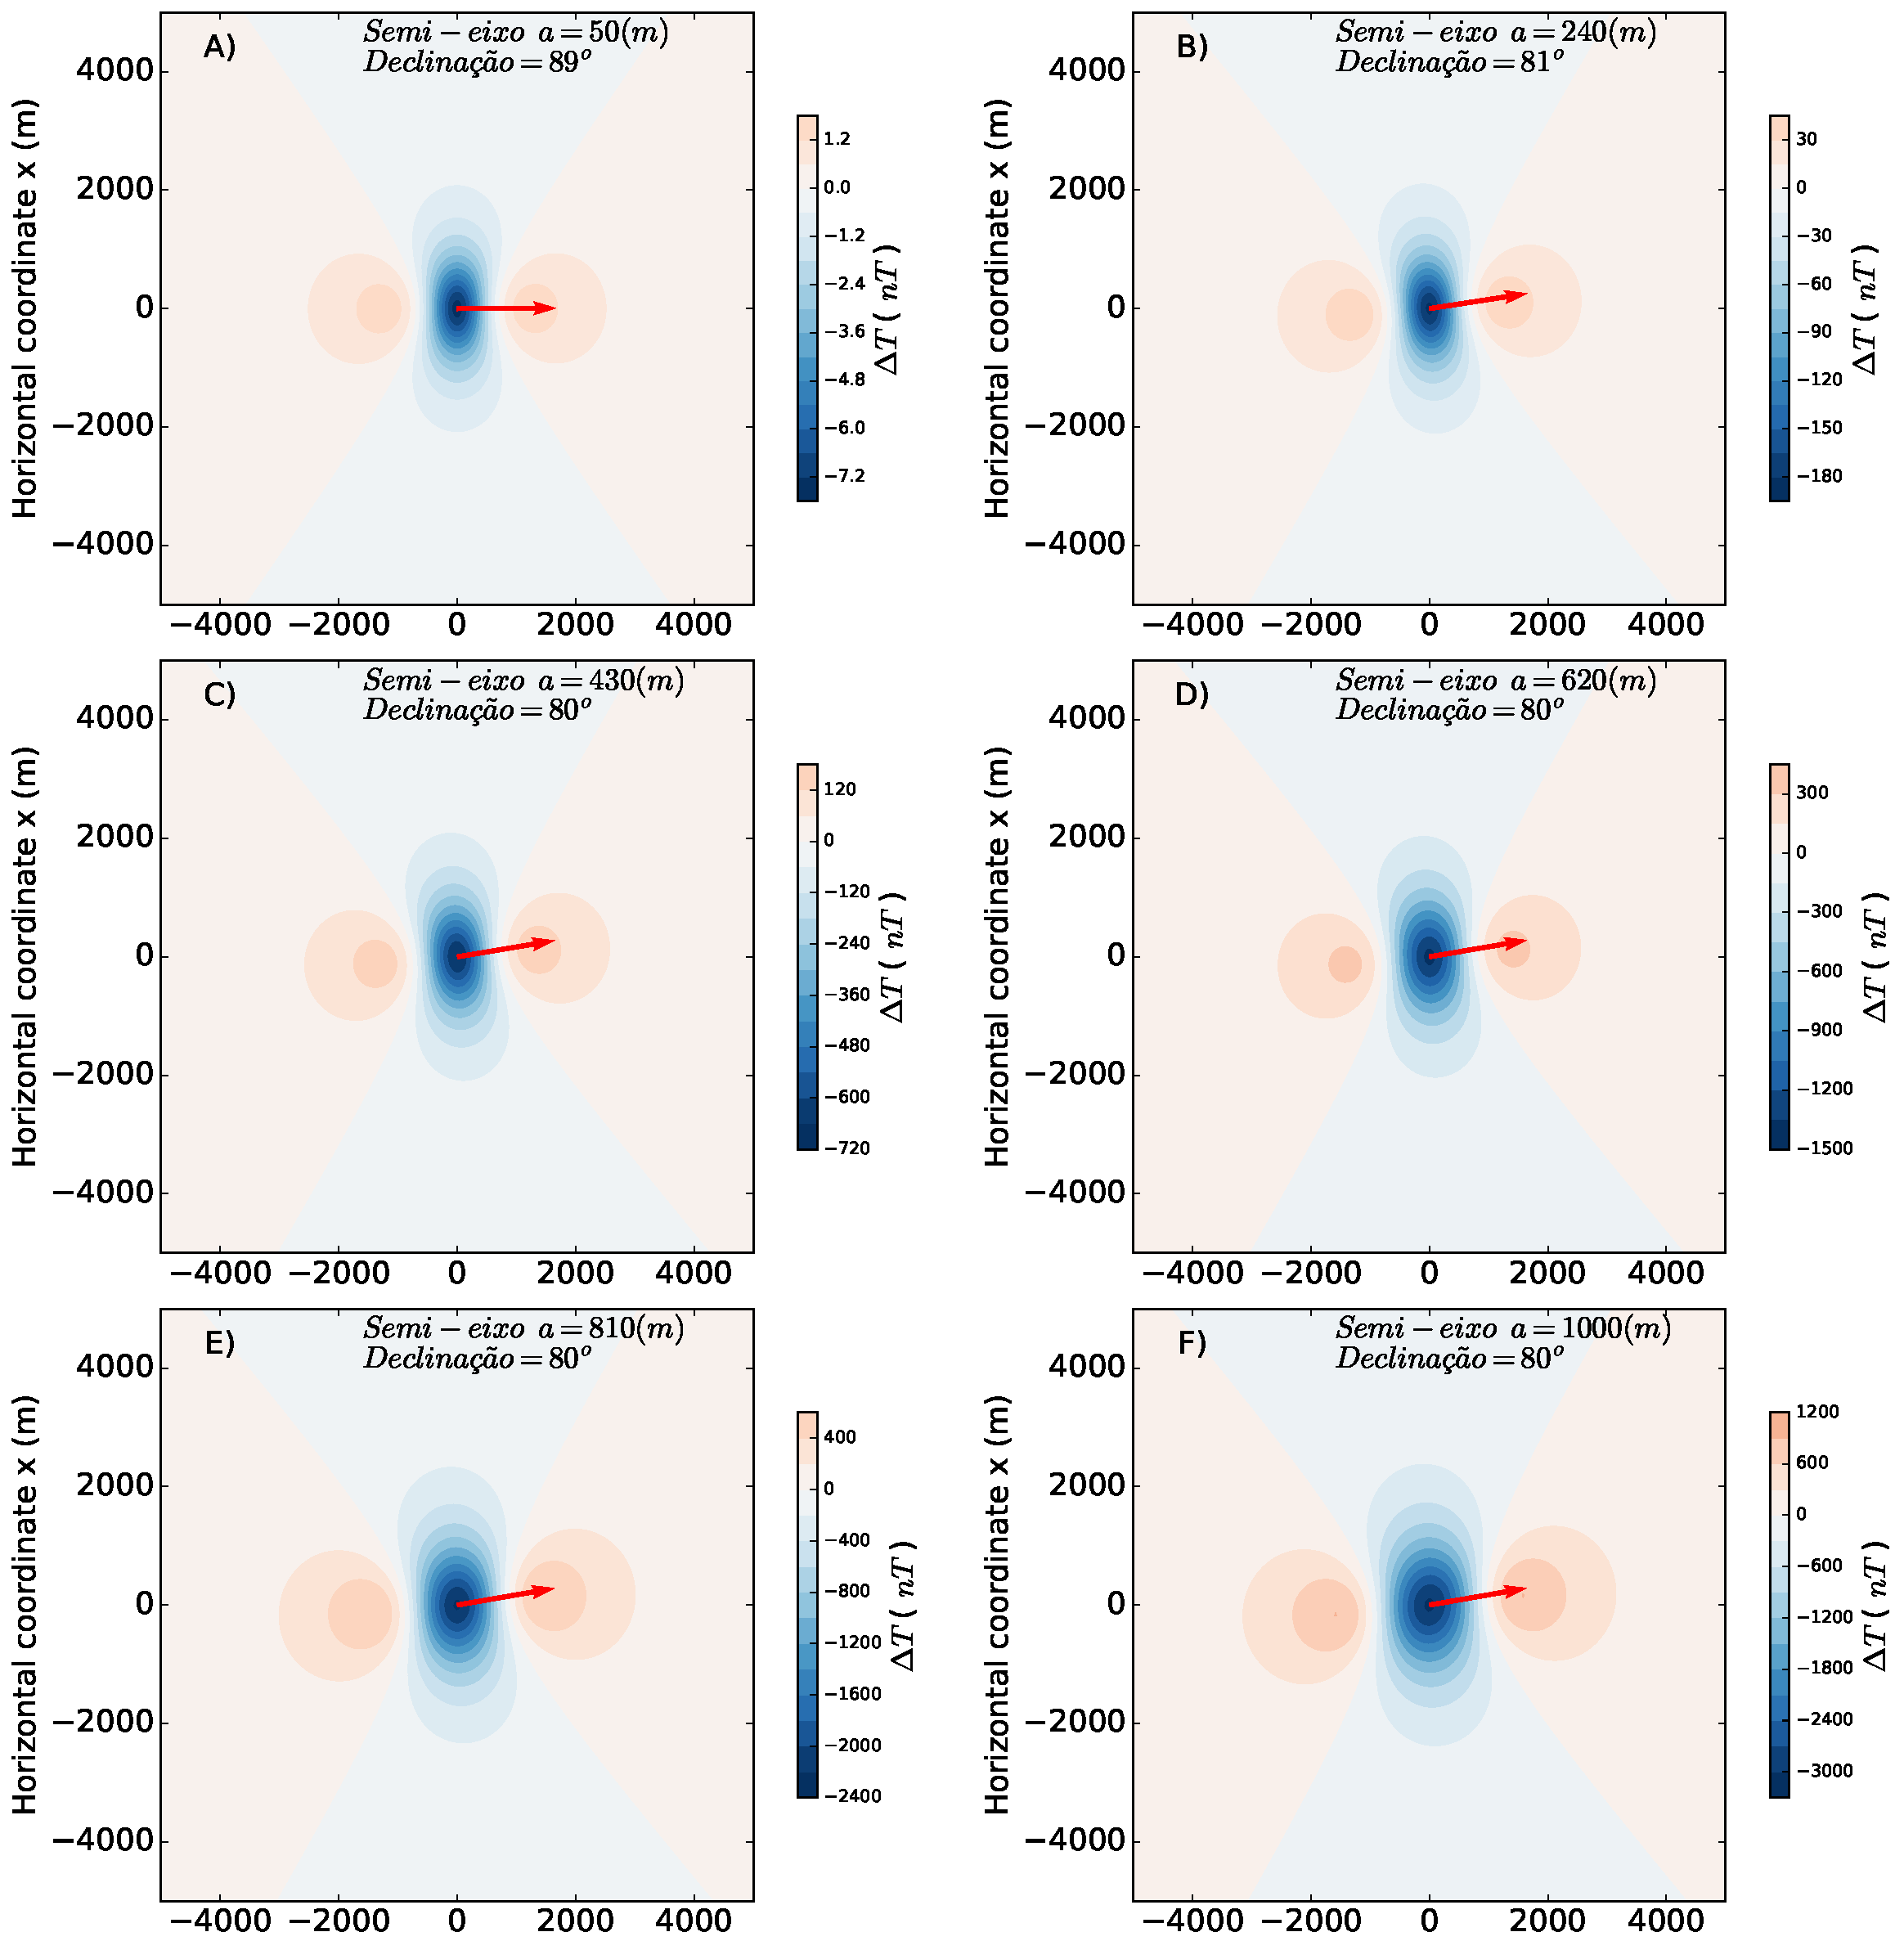
\includegraphics[width=16 cm,height=16 cm]{figures/ellipsoid_shape_iso2}
	\caption[Simulação, da mudança do vetor de magnetização resultante, de um elipsoide triaxial com o aumento do semi-eixo maior.]{Simulação, da mudança do vetor de magnetização resultante, de um elipsoide triaxial com o aumento do semi-eixo maior. O elipsoide está imerso em um campo externo constante de declinação $90^o$, possui susceptibilidade constante e direcionado com um azimute de $80^o$. Ao longo da sequência das figuras, seu semi-eixo maior aumenta de proporção em relação aos demais (variando entre 50 e 3000 m.). Nota-se a tendência do vetor de magnetização resultante (seta em vermelho) em se alinhar com o semi-eixo maior. Diferente da figura anterior, houve pouca mudança na declinação devido ao alinhamento do elipsoide com a campo externo.}
	\label{fig:ellipsoid_shape_iso80}
\end{figure}
  \chapter{Conclusões}

Esta dissertação apresenta uma revisão da vasta literatura sobre a modelagem magnética de elipsoides triaxiais, prolatos e oblatos, com orientação espacial arbitrária, suscetibilidade anisotrópica e magnetização remanente. Conjuntamente, apresenta uma forma alternativa de determinar a suscetibilidade isotrópica a partir da qual a desmagnetização deve ser considerada na modelagem e também a implementação de uma série de rotinas para o cálculo do campo magnético de corpos elipsoidais.

A modelagem direta do campo magnético gerado por fontes elipsoidais se mostrou satisfatória para os testes conduzidos neste trabalho. As componentes do campo magnético e a anomalia de campo total foram calculadas conforme o esperado para as três implementações propostas: para elipsoides triaxiais, prolatos e oblatos.
As validações das rotinas desenvolvidas neste trabalho foram feitas comparando-se as anomalias de campo total produzida por corpos com formato similar e localizados na mesma posição. As comparações foram feitas utilizando-se: i) um elipsoide triaxial e uma esfera, ii) um elipsoide triaxial e um elipsoide prolato e iii) um elipsoide triaxial e um elipsoide oblato. Os dados produzidos pelos elipsoides foram calculados com as rotinas desenvolvidas neste trabalho. Já os dados produzidos pela esfera foram calculados com o pacote Fatiando a Terra. Em todos os casos, as anomalias calculadas ficaram muito próximas entre si.

Outra simulação mostrou que os fatores de desmagnetização calculados para todos os tipos de elipsoide são i) diferentes  uns dos outros quando os semi-eixos dos elipsoides têm valores diferentes entre si e ii) tendem a $1/3$ quando o tamanho dos semi-eixos dos elipsoides são próximos uns aos outros.

Testes numéricos mostraram a mudança da direção do vetor de magnetização resultante em função da intensidade da susceptibilidade isotrópica. Estes testes ilustraram o critério alternativo proposto nesta dissertação para determinar o valor de suscetibilidade isotrópica a partir do qual a desmagnetização deve ser levada em consideração na modelagem magnética de corpos elipsoidais. Este critério é baseado no conhecimento prévio sobre a forma do corpo e no máximo erro relativo permitido na magnetização. Este critério é uma alternativa ao valor de 0,1 SI que tem sido utilizado de forma empírica pela comunidade geocientífica.

As rotinas desenvolvidas aqui se mostraram eficazes para calcular, de forma relativamente simples, o campo magnético produzido por múltiplos corpos. Estas rotinas foram desenvolvidas com base no pacote \textit{Fatiando a Terra} com o intuito de torná-las acessíveis para a comunidade científica. As rotinas estão disponibilizadas livremente no seguinte repositório no GitHub: https://github.com/DiegoTaka/ellipsoid-magnetic.

Futuramente estas rotinas poderão ser utilizadas tanto para modelar situações geológicas reais quanto para ensino. Estudos teóricos também poderão ser feitos para determinar o valor de suscetibilidade isotrópica a partir do qual a desmagnetização pode ser negligenciada com base no erro relativo máximo permitido no campo magnético calculado. As rotinas também poderão ser utilizadas para estudos de inversão magnética, podendo-se estimar diversos parâmetros como o vetor de magnetização, semi-eixos e as orientações angulares do corpo elipsoidal.


%  \chapter{Conclusões}


  \backmatter
  \bibliographystyle{on-plain}
  \bibliography{references}

  \appendix
  \chapter{Relação entre as derivadas das funções $f(\mathbf{r})$ e $\tilde{f}(\tilde{\mathbf{r}})$}

Sendo $\tilde{f}(\tilde{\mathbf{r}})$ a função escalar obtida transformando
$f(\mathbf{r})$ (Eq. \ref{eq:f}) do sistema de coordenas principal para um 
sistema de coordenadas local, por conveniência, reescreveremos a Eq. 
\ref{eq:coord_transformation} como:
\begin{equation}
\tilde{r}_{k} = v_{k1} \, r_{1} + v_{k2} \, r_{2} + v_{k3} \, r_{3} + c_{k} \: ,
\label{eq:r-tilde-k}
\end{equation}
em que $\tilde{r}_{k}$, $k = 1, 2, 3$, são os elementos do vetor posição
transformado $\tilde{\mathbf{r}}$ (Eq. \ref{eq:coord_transformation}),
$r_{j}$, $j = 1, 2, 3$, são os elementos do vetor posição
$\mathbf{r}$ (Eq. \ref{eq:ellipsoid_surface}),
$v_{kj}$, $j = 1, 2, 3$, são os elementos da matriz
$\mathbf{V}$ (Eq. \ref{eq:V_triaxial_prolate}),
e $c_{k}$ é uma constante definida pelas coordenadas
$x_{c}$, $y_{c}$, e $z_{c}$ do centro do corpo elipsoidal.

Considerando as funções $f(\mathbf{r})$ 
(Eq. \ref{eq:f}) e $\tilde{f}(\tilde{\mathbf{r}})$
calculadas no mesmo ponto, mas em diferentes sistemas
de coordenas, temos:
\begin{equation*}
\frac{\partial f(\mathbf{r})}{\partial r_{j}} = 
\frac{\partial \tilde{f}(\tilde{\mathbf{r}})}{\partial \tilde{r}_{1}} \,
\frac{\partial \tilde{r}_{1}}{\partial r_{j}} +
\frac{\partial \tilde{f}(\tilde{\mathbf{r}})}{\partial \tilde{r}_{2}} \,
\frac{\partial \tilde{r}_{2}}{\partial r_{j}} +
\frac{\partial \tilde{f}(\tilde{\mathbf{r}})}{\partial \tilde{r}_{3}} \,
\frac{\partial \tilde{r}_{3}}{\partial r_{j}} \: ,
\quad j = 1, 2, 3 \: ,
\end{equation*}
que, da Eq. \ref{eq:r-tilde-k}, pode ser dada por:
\begin{equation}
\frac{\partial f(\mathbf{r})}{\partial r_{j}} = 
v_{j1} \, \frac{\partial \tilde{f}(\tilde{\mathbf{r}})}{\partial \tilde{r}_{1}} +
v_{j2} \, \frac{\partial \tilde{f}(\tilde{\mathbf{r}})}{\partial \tilde{r}_{2}} +
v_{j3} \, \frac{\partial \tilde{f}(\tilde{\mathbf{r}})}{\partial \tilde{r}_{3}} \: ,
\quad j = 1, 2, 3 \: .
\label{eq:df_drj}
\end{equation}

Derivando $\frac{\partial f(\mathbf{r})}{\partial r_{j}}$
(Eq. \ref{eq:df_drj}) com respeito ao $i$-ésimo elemento 
$r_{i}$ do vetor posição $\mathbf{r}$ (Eq. \ref{eq:ellipsoid_surface}),
obtemos:
\begin{equation}
\begin{split}
\frac{\partial^{2} f(\mathbf{r})}{\partial r_{i} \, \partial r_{j}} &=
v_{j1} \, \frac{\partial}{\partial r_{i}} 
\left( \frac{\partial \tilde{f}(\tilde{\mathbf{r}})}{\partial \tilde{r}_{1}} \right) +
v_{j2} \, \frac{\partial}{\partial r_{i}} 
\left( \frac{\partial \tilde{f}(\tilde{\mathbf{r}})}{\partial \tilde{r}_{2}} \right) +
v_{j3} \, \frac{\partial}{\partial r_{i}} 
\left( \frac{\partial \tilde{f}(\tilde{\mathbf{r}})}{\partial \tilde{r}_{3}} \right) \\
&= v_{j1} \, \left( 
\frac{\partial^{2} \tilde{f}(\tilde{\mathbf{r}})}
{\partial \tilde{r}_{1} \, \partial \tilde{r}_{1}} \, v_{i1} + 
\frac{\partial^{2} \tilde{f}(\tilde{\mathbf{r}})}
{\partial \tilde{r}_{2} \, \partial \tilde{r}_{1}} \, v_{i2} + 
\frac{\partial^{2} \tilde{f}(\tilde{\mathbf{r}})}
{\partial \tilde{r}_{3} \, \partial \tilde{r}_{1}} \, v_{i3} 
\right) + \\
&+ v_{j2} \, \left( 
\frac{\partial^{2} \tilde{f}(\tilde{\mathbf{r}})}
{\partial \tilde{r}_{1} \, \partial \tilde{r}_{2}} \, v_{i1} + 
\frac{\partial^{2} \tilde{f}(\tilde{\mathbf{r}})}
{\partial \tilde{r}_{2} \, \partial \tilde{r}_{2}} \, v_{i2} + 
\frac{\partial^{2} \tilde{f}(\tilde{\mathbf{r}})}
{\partial \tilde{r}_{3} \, \partial \tilde{r}_{2}} \, v_{i3} 
\right) + \\
&+ v_{j3} \, \left( 
\frac{\partial^{2} \tilde{f}(\tilde{\mathbf{r}})}
{\partial \tilde{r}_{1} \, \partial \tilde{r}_{3}} \, v_{i1} + 
\frac{\partial^{2} \tilde{f}(\tilde{\mathbf{r}})}
{\partial \tilde{r}_{2} \, \partial \tilde{r}_{3}} \, v_{i2} + 
\frac{\partial^{2} \tilde{f}(\tilde{\mathbf{r}})}
{\partial \tilde{r}_{3} \, \partial \tilde{r}_{3}} \, v_{i3} 
\right) \\
&= \left[ \begin{array}{ccc}
v_{j1} & v_{j2} & v_{j3}
\end{array} \right] \tilde{\mathbf{F}}(\tilde{\mathbf{r}})
\left[ \begin{array}{c}
v_{i1} \\ v_{i2} \\ v_{i3}
\end{array} \right]
\end{split} \: ,
\label{eq:d2f-dridrj}
\end{equation}
em que $\tilde{\mathbf{F}}(\tilde{\mathbf{r}})$ é uma matriz $3 \times 3$, cujo $ij$-ésimo elemento é 
$\frac{\partial^{2} \tilde{f}(\tilde{\mathbf{r}})}
{\partial \tilde{r}_{i} \, \partial \tilde{r}_{j}}$.
Da Eq. \ref{eq:d2f-dridrj}, obtemos:
\begin{equation}
\mathbf{F}(\mathbf{r}) = \mathbf{V} \, 
\tilde{\mathbf{F}}(\tilde{\mathbf{r}}) \, \mathbf{V}^{\top} \: ,
\label{eq:F-V-F-tilde-VT}
\end{equation}
onde $\mathbf{F}(\mathbf{r})$ é uma matriz $3 \times 3$, cujo $ij$-ésimo elemento é 
$\frac{\partial^{2} f(\mathbf{r})}
{\partial r_{i} \, \partial r_{j}}$ e
$\mathbf{V}$ é definido pelas Eq. 
\ref{eq:V_triaxial_prolate}, dependendo do tipo de
elipsoide. Como pode ter notada, as matrizes $\mathbf{F}(\mathbf{r})$ e
$\tilde{\mathbf{F}}(\tilde{\mathbf{r}})$ representam as Hessianas
das funções $f(\mathbf{r})$ (Eq. \ref{eq:f})
e $\tilde{f}(\tilde{\mathbf{r}})$, respectivamente.
Além disso, o tensor de depolarização $\mathbf{N}(\mathbf{r})$
(Eq. \ref{eq:H-M-uniform}) pode se 
reescrito usando a matriz $\mathbf{F}(\mathbf{r})$
como:
\begin{equation}
\mathbf{N}(\mathbf{r}) = - \frac{1}{4 \pi} \mathbf{F}(\mathbf{r}) \: .
\label{eq:N-F}
\end{equation}
Usando apropriadamente a ortogonalidade de matrizes
$\mathbf{V}$,podemos reescrever a Eq. \ref{eq:F-V-F-tilde-VT}
como:
\begin{equation}
\tilde{\mathbf{F}}(\tilde{\mathbf{r}}) = \mathbf{V}^{\top} \, 
\mathbf{F}(\mathbf{r}) \, \mathbf{V} \: .
\label{eq:F-tilde-VT-F-V}
\end{equation}
Finalmente, multiplicando os dois lados da Eq. \ref{eq:F-tilde-VT-F-V}
por $-\frac{1}{4 \pi}$ e usando a Eq. \ref{eq:N-F},
nós concluímos que 
\begin{equation}
\tilde{\mathbf{N}}(\tilde{\mathbf{r}}) = 
\mathbf{V}^{\top} \, \mathbf{N}(\mathbf{r}) \, \mathbf{V} \: .
\label{eq:N-tilde-VT-N-V}
\end{equation}
  \chapter{Parâmetro $\lambda$ e suas derivadas espaciais}

Aqui, mostramos o raciocínio apresentado por \citet{webster1904}
para análise do parâmetro $\lambda$ que define os elipsoides triaxiais (Eq. \ref{eq:lambda-triaxial-ell}), prolatos e oblatos (Eq. \ref{eq:lambda-prolate-ell}).

\section{Parâmetro $\lambda$ definido para os elipsoides triaxiais}

Consideremos um elipsoide de semi-eixos $a$, $b$ e $c$ orientados ao longo dos eixos
$\tilde{x}$, $\tilde{y}$, e $\tilde{z}$, respectivamente, no seu sistema de coordenadas
local, em que $a > b > c > 0$. Este elipsoide é definido pela seguinte equação:
\begin{equation}
\frac{\tilde{x}^{2}}{a^{2}} + \frac{\tilde{y}^{2}}{b^{2}} + \frac{\tilde{z}^{2}}{c^{2}} = 1 \: .
\label{eq:reference-triaxial-ell}
\end{equation}
Uma superfície quádrica (e.g., elipsoide, hiperboloides de uma camada ou 
hiperboloides de duas camadas) que é confocal à um elipsoide definido pela
Eq. \ref{eq:reference-triaxial-ell} pode ser descrito como:
\begin{equation}
\frac{\tilde{x}^{2}}{a^{2} + u} + \frac{\tilde{y}^{2}}{b^{2} + u} + \frac{\tilde{z}^{2}}{c^{2} + u} = 1 \: ,
\label{eq:quadric-confocal-triaxial-ell}
\end{equation}
em que $u$ é um número real. A equação \ref{eq:quadric-confocal-triaxial-ell}
representa um elipsoide para $u$ que satisfaz a condição:
\begin{equation}
u + c^{2} > 0 \: .
\label{eq:condition-triaxial-ell}
\end{equation}

Dado $a$, $b$, $c$, e um $u$ que satisfaz \ref{eq:condition-triaxial-ell}, 
podemos usar \ref{eq:quadric-confocal-triaxial-ell} para determinar um conjunto 
de pontos $(x, y, z)$ situado na superfície de um elipsoide que é confocal aquele
definido pela Eq. \ref{eq:reference-triaxial-ell}. 
Considere o problema em determinar o elipsoide que é confocal com aquele definido em
\ref{eq:reference-triaxial-ell} e que passa por um ponto particular $(\tilde{x}, \tilde{y}, \tilde{z})$.
Este problema consiste em determinar o número real $u$ que, dado  $a$, $b$, $c$, $\tilde{x}$, $\tilde{y}$, e $\tilde{z}$,
satisfaz a Eq. \ref{eq:quadric-confocal-triaxial-ell} e
a condição expressa pela Eq. \ref{eq:condition-triaxial-ell}.
Rearranjando a Eq. \ref{eq:quadric-confocal-triaxial-ell}, obtemos a seguinte equação cúbica para $u$
\begin{equation}
p(u) = (a^{2} + u)(b^{2} + u)(c^{2} + u) - (b^{2} + u)(c^{2} + u) \, \tilde{x}^{2}
- (a^{2} + u)(c^{2} + u) \, \tilde{y}^{2} - (a^{2} + u)(b^{2} + u) \, \tilde{z}^{2} \: .
\label{eq:cubic-equation-triaxial-ell}
\end{equation}
Esta equação cúbica mostra que:
\begin{equation}
u = \begin{cases}
d \to \infty \: &, \quad p(u) > 0 \\
-c^{2} \: &, \quad p(u) < 0 \\
-b^{2} \: &, \quad p(u) > 0 \\
-a^{2} \: &, \quad p(u) < 0
\end{cases} \: .
\label{eq:cubic-equation-signals-triaxial-ell}
\end{equation}
Note que, de acordo com \ref{eq:cubic-equation-signals-triaxial-ell},
a menor, a intermediária e a maior raiz da equação cúbica
$p(u)$ (Eq. \ref{eq:cubic-equation-triaxial-ell}) estão 
localizadas, respectivamente, nos intervalos $[ -a^{2} \, , -b^{2} ]$,
$[ -b^{2} \, , -c^{2} ]$ and $[ -c^{2} \, , \infty [$.
Lembremos que estamos procurando um $u$ que satisfaz a condição
expressa pela Eq. \ref{eq:condition-triaxial-ell}. 
Consequentemente, de acordo com a análise de sinal mostrada na Eq.
\ref{eq:cubic-equation-signals-triaxial-ell}, estamos interessados na 
maior raiz $\lambda$ da equação cúbica $p(u)$ (Eq.
\ref{eq:cubic-equation-triaxial-ell}).

Da Eq. \ref{eq:cubic-equation-triaxial-ell}, obtemos uma mais simples
dada por:
\begin{equation}
p(u) =  u^{3} + p_{2} \, u^{2} + p_{1} \, u + p_{0} \: ,
\label{eq:cubic-equation-triaxial-ell-simpler}
\end{equation}
em que
\begin{equation}
p_{2} = a^{2} + b^{2} + c^{2} - \tilde{x}^{2} - \tilde{y}^{2} - \tilde{z}^{2} \: ,
\label{eq:p2-triaxial-ell}
\end{equation}
\begin{equation}
p_{1} = b^{2} \, c^{2} + a^{2} \, c^{2} + a^{2} \, b^{2} 
- (b^{2} + c^{2}) \, \tilde{x}^{2}
- (a^{2} + c^{2}) \, \tilde{y}^{2} 
- (a^{2} + b^{2}) \, \tilde{z}^{2}
\label{eq:p1-triaxial-ell}
\end{equation}
e
\begin{equation}
p_{0} =  a^{2} \, b^{2} \, c^{2} - b^{2} \, c^{2} \, 
\tilde{x}^{2} - a^{2} \, c^{2} \, \tilde{y}^{2} - a^{2} \, 
b^{2} \, \tilde{z}^{2} \: .
\label{eq:p0-triaxial-ell}
\end{equation}
Finalmente, das Eqs. \ref{eq:p2-triaxial-ell}, 
\ref{eq:p1-triaxial-ell} e \ref{eq:p0-triaxial-ell},
a maior raiz $\lambda$ de $p(u)$ 
(Eq. \ref{eq:cubic-equation-triaxial-ell-simpler}) pode ser
calculada como mostra \citep{weisstein2017}:
\begin{equation}
\lambda = 2 \, \sqrt{-Q} \, \cos \left( \frac{\theta}{3}\right) - \frac{p_{2}}{3} \: ,
\label{eq:lambda-triaxial-ell}
\end{equation}
em que
\begin{equation}
\theta = \cos^{-1} \left( \frac{R}{\sqrt{Q^{3}}} \right) \: ,
\label{eq:theta-triaxial-ell}
\end{equation}
\begin{equation}
Q = \frac{3 \, p_{1} - p_{2}^{2}}{9}
\label{eq:Q-triaxial-ell}
\end{equation}
e
\begin{equation}
R = \frac{9 \, p_{1} \, p_{2} - 27 \, p_{0} - 2 \, p_{2}^{3}}{54} \: .
\label{eq:R-triaxial-ell}
\end{equation}

\section{Parâmetro $\lambda$ que define os elipsoides prolatos e oblatos}

Vamos agora considerar um elipsoide prolato de semi-eixos $a$, $b$, 
$c$ orientados ao longo dos eixos $\tilde{x}$, $\tilde{y}$, e 
$\tilde{z}$, respectivamente, de seu sistema de coordenadas local, em que $a > b = c > 0$.
Neste caso, a equação que define a superfície do elipsoide é obtida substituindo
$c = b$ na Eq. \ref{eq:reference-triaxial-ell}. Consequentemente, a equação que define a
respectiva superfície quádrica confocal é dada por:
\begin{equation}
\frac{\tilde{x}^{2}}{a^{2} + u} + \frac{\tilde{y}^{2} + \tilde{z}^{2}}{b^{2} + u} = 1
\label{eq:quadric-confocal-prolate-ell}
\end{equation}
e a nova condição que a variável $u$ precisa satisfazer para que a
Eq. \ref{eq:quadric-confocal-prolate-ell} represente um elipsoide é:
\begin{equation}
u + b^{2} > 0 \: .
\label{eq:condition-prolate-ell}
\end{equation}

Similarmente ao caso do elipsoide triaxial apresentado na subseção anterior,
estamos interessados em determinar o número real $u$ que, dado $a$, $b$, $\tilde{x}$, $\tilde{y}$,
e $\tilde{z}$, satisfaz a Eq. \ref{eq:quadric-confocal-prolate-ell} e a condição expressa por
Eq. \ref{eq:condition-prolate-ell}. Da Eq. \ref{eq:quadric-confocal-prolate-ell}, obtemos a
seguinte equação quádrica para $u$:
\begin{equation}
p(u) = (a^{2} + u)(b^{2} + u) - (b^{2} + u) \, \tilde{x}^{2}
- (a^{2} + u) \, (\tilde{y}^{2} + \tilde{z}^{2}) \: .
\label{eq:quadratic-equation-prolate-ell}
\end{equation}
Esta equação mostra que:
\begin{equation}
u = \begin{cases}
d \to \infty \: &, \quad f(\rho) > 0 \\
-b^{2} \: &, \quad f(\rho) < 0 \\
-a^{2} \: &, \quad f(\rho) > 0
\end{cases}
\label{eq:quadratic-equation-signals-prolate-ell}
\end{equation}
e, consequentemente, que duas raízes se situam nos intervalos $[ -a^{2} \, , -b^{2} ]$ 
e $[ -b^{2} \, , \infty [$. Assim, de acordo com a condição estabelecida pela
Eq. \ref{eq:condition-prolate-ell} e a análise de sinais mostrada na Eq. \ref{eq:quadratic-equation-signals-prolate-ell},
estamos interessados na maior raiz $\lambda$ da equação quádrica $p(u)$ (Eq. \ref{eq:quadratic-equation-prolate-ell}).

Manipulando corretamente a Eq. \ref{eq:quadratic-equation-prolate-ell}, obtemos uma mais simples dada por:
\begin{equation}
p(u) =  u^{2} + p_{1} \, u + p_{0} \: ,
\label{eq:quadratic-equation-prolate-ell-simpler}
\end{equation}
em que
\begin{equation}
p_{1} = a^{2} + b^{2} - \tilde{x}^{2} - \tilde{y}^{2} - \tilde{z}^{2}
\label{eq:p1-prolate-ell}
\end{equation}
e
\begin{equation}
p_{0} =  a^{2} \, b^{2} 
- b^{2} \, \tilde{x}^{2} 
- a^{2} \left( \tilde{y}^{2} + \tilde{z}^{2} \right) \: .
\label{eq:p0-prolate-ell}
\end{equation}
Finalmente, usando as Eqs. \ref{eq:p1-prolate-ell} e
\ref{eq:p0-prolate-ell}, a maior raiz $\lambda$ de $p(u)$ 
(Eq. \ref{eq:quadratic-equation-prolate-ell-simpler}) pode ser 
facilmente calculada como:
\begin{equation}
\lambda = \frac{-p_{1} + \sqrt{p_{1}^{2} - 4 \, p_{0}}}{2} \: .
\label{eq:lambda-prolate-ell}
\end{equation}

Para o caso do elipsoide oblato, o procedimento para determinar o parâmetro
$\lambda$ é muito similar para os elipsoides prolatos. Os semi-eixos $a$, $b$, $c$
do elipsoide oblato são definidos de forma que $b = c > a > 0$ e a condição que a variável $u$
deve satisfazer é $u + a^{2} > 0$. Neste caso, as duas raízes que resultam da equação quádrica situam-se
nos intervalos $[ -b^{2} \, , -a^{2} ]$ e $[ -a^{2} \, , \infty [$. Consequentemente, continuamos interessados 
na maior raiz da equação quádrica para a variável $u$, que também é calculada usando a Eq. \ref{eq:lambda-prolate-ell}.

\section{Derivadas espaciais do parâmetro $\lambda$}

A modelagem magnética dos elipsoides triaxiais, prolatos e oblatos necessitam além do parâmetro
$\lambda$ definidos pelas Eqs. \ref{eq:lambda-triaxial-ell} e \ref{eq:lambda-prolate-ell}, das suas derivadas
com respeito as coordenadas espaciais $\tilde{x}$, $\tilde{y}$, and $\tilde{z}$.
Felizmente, as derivadas espaciais do parâmetro $\lambda$ podem ser calculadas de forma bastante
similares para todos os tipos de elipsoides.

Vamos considerar um elipsoide triaxial primeiro. Neste caso, as derivas espaciais de $\lambda$
são dadas por:
\begin{equation}
\frac{\partial \lambda}{\partial \tilde{r}_{j}} =
\frac{\frac{2 \, \tilde{r}_{j}}{\left( e_{j}^{2} + \lambda \right)}}{
	\left( \frac{\tilde{x}}{a^{2} + \lambda}\right)^{2} +
	\left( \frac{\tilde{y}}{b^{2} + \lambda}\right)^{2} + 
	\left( \frac{\tilde{z}}{c^{2} + \lambda}\right)^{2}} \: , \quad j = 1, 2, 3 \: ,
\label{eq:dlambda}
\end{equation}
em que 
$\tilde{r}_{1} = \tilde{x}$, $\tilde{r}_{2} = \tilde{y}$, $\tilde{r}_{3} = \tilde{z}$,
$e_{1} = a$, $e_{2} = b$, and $e_{3} = c$.
Esta equação pode ser determinada diretamente da equação \ref{eq:quadric-confocal-triaxial-ell}.
As derivadas espaciais de $\lambda$ no caso dos elipsoides prolatos e oblatos podem ser calculados usando
a Eq. \ref{eq:dlambda} para o o caso particular em que $b = c$.

\end{document} 